\documentclass[MS,synopsis]{iitddiss}
\usepackage{times}
\usepackage{t1enc}
\usepackage{lipsum}
%\usepackage[backend=bibtex,sorting=none,style=numeric-comp]{biblatex}
%\bibliography{references.bib}

\usepackage{graphicx}
\usepackage{hyperref} % hyperlinks for references.
\usepackage{amsmath} % easier math formulae, align, subequations \ldots
\usepackage{graphicx}
\usepackage{epstopdf}

\title{Data Analysis for Predicting Instabilities in Power Systems}

\author{Aryan Ritwajeet Jha}
\entrynumber{2020EEY7525}
\advisor{Prof. Nilanjan Senroy}
\date{July 2022}
\department{Electrical Engineering}


\begin{document}

%\nocite{*}
\maketitle

\pagenumbering{arabic}
\setcounter{page}{0}

\newpage

\tableofcontents

\newpage

\section[Introduction to My Work]{Introduction}
\label{sec:introduction}

\begin{frame}[fragile]{Transient vs Steady State Stability}
	\begin{tabularx}{\textwidth}{
			@{\hspace{1.5em}}% Space for left bullet
			>{\leavevmode\raggedright}% Left bullet + formatting of column
			X% Left column specification
			@{\quad\hspace{1.5em}}% Space between columns + right bullet space
			>{\leavevmode\raggedright\arraybackslash}% Right bullet + formatting of column
			X% Right column specification
			@{}% No column space on right
		}
		\textbf{Transient Stability} & \textbf{Steady State Stability}\\
		\toprule
		A sudden, out-of-trend, high magnitude change in a state variable(s) causes blackouts. & 
		Accumulation of several seemingly minor trends in state variables over time, ultimately leading to a \textcolor{red}{critical point} where a small change could cause blackouts.\\
		Chief parameters of concern are ROCOF, frequency nadir, steady-state frequency deviation. & 
		\textcolor{red}{Autocorrelation} and covariance are some of the commonly used parameters for prognosis.\\
		Inertia is a fundamental parameter here. & Inertia plays a minor role here.\\
		\bottomrule
	\end{tabularx}
\end{frame}

\begin{frame}{Bifurcations and Critical Slowing Down}
	\textbf{Bifurcation}: A qualitative change in the `motion' of a dynamical System due to a quantitative change in one of its parameters. Serious bifurcations, called \textcolor{red}{Critical Bifurcations}, cause the system to become unstable from stable.
\end{frame}

\begin{frame}{Bifurcations and Critical Slowing Down}
	\textbf{Critical Slowing Down}: Dynamical Systems exhibit early statistical warning signs before collapsing:
	
	\begin{itemize}
		\item Increased recovery times from perturbations.
		\item Increased signal variance from the mean trajectory.
		\item Increased flicker and asymmetry in the signal
	\end{itemize}

The above three properties can be identified by increasing variance and autocorrelation in time-series measurements taken from the system.
\end{frame}


\section{Literature Review}[Literature Review]
\label{sec:litt}

\section[Motivation and Objectives]{Objectives}
\label{sec:obj}

\lipsum[1]

\section[Theory]{Theory}
\label{sec:theory}

\textbf{Detrended Fluctuation Analysis}: A method of analyzing real-world time series for self-affinity, i.e. how correlated a signal's future value is to it's past values. Say, $x(t)$ is a signal from a natural process, then in order to detrend it, it can first be passed via a low-pass filter $\verb|LPF|$ to obtain \verb|LPF|$(x(t))$ and the resultant signal be subtracted from the original in order to obtain the detrended version of the natural process signal $\tilde{x}(t)$ or $d(x(t))$:
\begin{equation}
	\tilde{x}(t) \verb| or | d(x(t)) = x(t) - \verb|LPF|(x(t))
\end{equation}

\textbf{Autocorrelation function}: A statistical measure of the correlation of a state variable with a time-lagged version of itself. 

\begin{equation}
	c(x(t), \tau) = \int_{-\infty}^{\infty}x(t)x(t+\tau)dt  
\end{equation}

In terms of discrete time functions, autocorrelation may be expressed as:
\begin{equation}
	c(x[n], \tau) =  \sum_{-\infty}^{\infty} x[n]x[n+\tau]
\end{equation}

It may be noted that the autocorrelation function of any time-varying variable has two degrees of freedom, the first being continuous time $t$ (or instance $n$ for discrete time functions) and the second parameter being the lag $\tau$, i.e. the time duration by which the time-varying variable is displaced/lagged against itself for performing the autocorrelation.

Since in this thesis the function is used in two ways where only one of the parameters is varying (with the other being kept constant) each time, two variations of the autocorrelation function with individual names are specified here:

\textbf{Fixed Time Autocorrelation}: Autocorrelation function computed over a snapshot of a time-varying variable over a fixed time window. The usage of Fixed Time Autocorrelation can be seen in the Offline Analysis chapter (Chapter \ref{sec:offline}) of this thesis.

\begin{equation}
	c(\tau) = \frac{\sum_{1}^{W_{total}-1} x[n]x[n+\tau]}{\sum_{1}^{W_{total}-1} x[n]^2} 
\end{equation}
 
 In this thesis, the window length $W_{total}$ ranges from months to years.
 
 \textbf{Fixed Lag Autocorrelation}: Autocorrelation function computed over a window running over a continuously generated stream of data in which the value of the lag $\tau$ is fixed. The usage of Fixed Lag Autocorrelation can be seen in the Online Analysis chapter (Chapter \ref{sec:online}) of this thesis.
 
 \begin{equation}
 	c(t)|_{\tau = \tau_{fixed}} = \frac{\sum_{i}^{i+W-1} x[n]x[n+\tau_{fixed}]}{\sum_{i}^{i+W-1} x[n]^2} 
 \end{equation}
 
 In this thesis, the window length used is $W=15$ seconds. The value of $\tau$ used is $\tau_{fixed}=1$ second.

\textbf{Variance}: Degree of overall deviation/fluctuation in the values of a data.

\begin{equation}
	\sigma^2(x) = E(x^2) - (E(x))^2 
\end{equation}
\hspace{75pt} where,
\begin{equation}
	E(x) = \frac{1}{W} \sum_{i}^{i+W-1} x[n]
\end{equation}

\textbf{Bifurcation Theory}: The concepts Bifurcations and Critical Bifurcations were used to explain why a small yet steady change in the parameters of a dynamical system (such as the power grid) can remain inconspicuous only to, upon reaching a `tipping' point or `Critical Transition', manifest as a sudden major upset to the `motion' of the dynamical system. The terms Bifurcations and Critical Bifurcations were used almost interchangeably, although technically only Critical Bifurcations are significant enough to alter the dynamics of a system from stable to unstable. Any dynamical system can be expressed as a set of differential algebraic equations. The  Figures \ref{fig:bifPitchforkSupercritical} and \ref{fig:bifPitchforkSubcritical} demonstrate this phenomena in a particular variation, the Pitchfork bifurcation.


\begin{figure}[!ht]
	\centering{
	\import{../figures/}{bifurcationPitchforkPdf.pdf_tex}
	}
	\caption{Bifurcation diagram for the normal form of the Supercritical Pitchfork Bifurcation $\frac{dx}{dt} = \mu x - x^3$. \\ For $\mu \leq 0$, the only stable equilibrium solution for the dynamical system (or fixed point) is $x=0$. Upon reaching the critical `tipping' point $\mu=0$, $x=0$ no longer remains a stable equilibrium path for the dynamical system and instead two different stable paths emerge: $x = \sqrt{+\mu}$ and $x = -\sqrt{\mu}$. Such a critical point, in which one stable path bifurcates into at least two distinct paths (which may or may not be stable) is called a bifurcation point and the phenomenon is known as `Critical Bifurcation'.}
	\label{fig:bifPitchforkSupercritical}
\end{figure}

\begin{figure}[!ht]
	\centering{
		\import{../figures/}{bifurcationPitchforkNegativePdf.pdf_tex}
	}
	\caption{Bifurcation diagram for the normal form of the Subcritical Pitchfork Bifurcation $\frac{dx}{dt} = \mu x + x^3$. \\ For $\mu \leq 0$, the only stable equilibrium solution (or fixed point) for the dynamical system is $x=0$. Upon reaching the critical `tipping' point $\mu=0$, three different equilibrium solutions (or fixed points) emerge: $x=0$, $x = \sqrt{+\mu}$ and $x = -\sqrt{\mu}$, none of which are stable. Here too, $\mu=0$ is a bifurcation point.}
	\label{fig:bifPitchforkSubcritical}
\end{figure}


\textbf{Critical Slowing Down}: The theory of Critical Slowing Down applies on dynamical systems on the verge of `tipping' or `bifurcation' and how they show warning signs before breaking down or descending into instability. These warning signs such as an `increased time to settle', `increased autocorrelation and variance of fluctuations', etc. \cite{schefferEarlyWarningSignalsForCriticalTransitions} can be statistically analyzed to predict the onset of such a bifurcation for a given system.
Autocorrelation $c(t, \tau)$ of any detrended physical/natural signal $\tilde{x}(t)$ or $d(x(t))$, should decrease exponentially as the time-lag $\tau$ is increased.

\textbf{Why do Autocorrelation and Variance increase with Critical Slowing Down?}:

The question may be divided into two parts:
\begin{enumerate}
	\item How does the autocorrelation of the perturbations of a system's state variables increase when the system is undergoing Critical Slowing Down?
	\item For a system with increasing autocorrelation of the perturbations its state variables, how does the variance of the perturbations also increase?
\end{enumerate}

As an answer to the first question, we may consider the example given in \cite{schefferEarlyWarningSignalsForCriticalTransitions}:

Let a dynamical system be represented by the differential function

\begin{equation}
	\label{eq:exampleDynamicalSystem}
	\frac{dx}{dt} = k(x-x_1)(x-x_2)
\end{equation}
where $k$ is a positive coefficient, $x_1$ and $x_2$ are parameters, possibly as result of inherent dynamics of the system infrastructure or an intentional control mechanism (in which case, they are also known as control parameters).

Let $x_1$ be the stable equilibrium point (or stable fixed point) and $x_2$ be the unstable equilibrium point (unstable fixed point	). This implies that $x_1 < x_2$ (one may easily prove this by taking the second derivatives of Equation \ref{eq:exampleDynamicalSystem} and checking for its sign at the fixed points).

Now if the system were to be perturbed at its stable fixed point $x_1$ by a small disturbance of $\Delta x$, the perturbed dynamical system could be expressed by a slight variation of Equation \ref{eq:exampleDynamicalSystem}:

\begin{equation}
	\frac{d(x_1+\Delta x)}{dt} = k(x_1+\Delta x-x_1)(x_1+\Delta x - x_2)
\end{equation}
\hspace{25pt} or,

\begin{equation}
	\frac{d(x_1)}{dt} + \frac{d(\Delta x)}{dt} = k(\Delta x)(\Delta x + x_1 - x_2)
\end{equation}
\hspace{25pt} or,

\NewDocumentCommand{\evalat}{sO{\big}mm}{%
	\IfBooleanTF{#1}
	{\mleft. #3 \mright|_{#4}}
	{#3#2|_{#4}}%
}
\begin{equation}
	\evalat[\bigg]{\frac{d(\Delta x)}{dt}}{x_1} = k\left\{(x_1-x_2)\Delta x + (\Delta x)^2\right\}
\end{equation}
\hspace{25pt} Ignoring the second order terms:

\begin{equation}
	\evalat[\bigg]{\frac{d(\Delta x)}{dt}}{x_1} = k(x_1-x_2)\Delta x
\end{equation}
\hspace{25pt} Since the perturbation $\Delta x$ is independent of the parameters $x_1$ and $x_2$, the above equation may be rewritten by replacing $k(x_1-x_2)$ with $\lambda_1$:

\begin{equation}
	\evalat[\bigg]{\frac{d(\Delta x)}{dt}}{x_1} = \lambda_1 \Delta x 
\end{equation}
Thus the perturbation may be expressed as an explicit time domain equation:
\begin{equation}
	\Delta x(t)|_{x_1} = \exp{(\lambda_1 t)}
\end{equation}
which has a recovery rate of $\lambda_1 = k(x_1-x_2)$. On the other hand, a perturbation at the unstable fixed point $x_2$ would become exponentially increasing.
\begin{equation}
	\evalat[\bigg]{\frac{d(\Delta x)}{dt}}{x_2} = \exp{(\lambda_2 t)}
\end{equation}
 \hspace{25pt} where $\lambda_2 = -\lambda_1 = -k(x_1-x_2)$
 
It may be seen from the above two equations representing the perturbations at the two fixed points that their recovery (or blow-up) rates depend on the difference in the values of the parameters $x_1$ and $x_2$. At the special case of $x_1 = x_2$, the fixed points exchange stability and the recovery rates tend to zero (Refer to the critical point $\mu$ in figures \ref{fig:bifPitchforkSupercritical} and \ref{fig:bifPitchforkSubcritical}) for an example of the phenomena in two variations of the Pitchfork Bifurcation).
 
The same reference \cite{schefferEarlyWarningSignalsForCriticalTransitions} also explains the increase of autocorrelation and variance when a dynamical system trends towards instability with the help of the example below:

Consider a discrete-time stochastic dynamical system with the vector of state variables being depicted by $x$. Let $x_n$ depict the value of the state variable vector $x$ at discrete time instance $n$.
Now, if an additive noise say, Gaussian noise, is added to the stochastic dynamical system at every discrete time interval $\Delta t$, the slightly perturbed set of state variables, say $x_{n+1}$, of the otherwise stable dynamical system, would attempt to return to the set of state variables before the perturbation $x_n$, with an exponential recovery speed.

\begin{equation}
	x_{n+1} - x_{n} = \exp{(\lambda \Delta t)}(x_{n+1}-x_{n}) + \zeta_n\sigma
\end{equation}

\hspace{25pt} where $\sigma$ is the standard deviation representing the stochastic noise (assumed Gaussian) inherent to the stochastic dynamical system and $\zeta_n$ represents a coefficient to $\sigma$ to model the magnitude of the stochastic noise at discrete-time instant $n$. $\lambda$ represents the rate of exponential recovery.

The term $x_{n+1} - x_{n}$ may then simply be replaced with term $y_{n+1}$ which depicts the deviation of the vector of state variables $x$ between discrete-time instances $n$ and $n+1$.

\begin{equation}
	y_{n+1} = \exp{(\lambda \Delta t)}y_n + \zeta_n
	\sigma
\end{equation}

Now if the time intervals between perturbations $\Delta t$ and the recovery rate $\lambda$ are independent of the state variables $x_{n}$ (and therefore their perturbations $y_{n}$), the above equation may be rewritten in the form of an autoregression model of the first order:

\begin{equation}
	\label{eq:autocorrNoConstant}
	y_{n+1} = \alpha y_{n} + \zeta_n\sigma
\end{equation}

The autocorrelation constant $\alpha \equiv \exp{(\lambda \Delta t)}$ is zero for a purely white gaussian noise and can be one or even greater for other kinds of highly correlated noises in stochastic processes such as brown noise (un-normalized data only).

For the general equation of a lag-1 autoregression:
\begin{equation}
	\label{eq:autocorrGeneral}
	y_{n+1} = \alpha_0 + \alpha y_{n} + \zeta_n\sigma
\end{equation} 
the expected value (mean) of $y_{n}$ may be computed using:
\begin{equation}
	\EX(y_{n+1}) = \EX(\alpha_0) + \EX(\alpha y_{n}) + \EX(\zeta_n \sigma)
\end{equation}
\hspace{25pt} or,
\begin{equation}
	\mu = \alpha_0 + \alpha\mu + 0
\end{equation}
\hspace{25pt} or
\begin{equation}
	\label{eq:meanFormulaGeneral}
	\mu = \frac{\alpha_0}{1-\alpha}
\end{equation}

Thus, if $\alpha_0 = 0$, as in Equation \ref{eq:autocorrNoConstant}, the mean of autoregression $\mu$ will also be zero.

The variance of $y_{n}$, $\sigma^2_{y_{n}}$ may be computed using the formula for variance:

\begin{equation}
	\sigma^2_{y_{n}} = \EX(y^2_{n}) - \left(\EX(y_{n})\right)^2
\end{equation} 	
\hspace{25pt} or,
\begin{equation}
	\label{eq:sigmaComputationBegins}
	\sigma^2_{y_{n}} = \EX(y^2_{n}) - \mu^2
\end{equation}

For computing the first term of the RHS of Equation \ref{eq:sigmaComputationBegins}, Equation \ref{eq:autocorrGeneral} may once again be utilized by taking the squares on both of its sides:

\begin{equation}
	y^2_{n+1} = \alpha^2_0 + \alpha^2 y^2_{n} + \zeta^2_n \sigma^2 + 2\alpha_0 \alpha y_{n} + 2\alpha_0 \zeta_n \sigma + 2\alpha y_{n} \zeta_n \sigma
\end{equation}
\hspace{25pt} or,
\begin{equation}
	\EX(y^2_{n}) = \alpha^2_0 + \alpha^2 \EX(y^2_{n}) + \zeta^2_{n} \sigma^2 + 2\alpha_0\alpha\EX(y_{n}) + 0 + 0
\end{equation}
\hspace{25pt} or,
\begin{equation}
	\EX(y^2_{n}) = \frac{\alpha^2_{0} + 2\alpha_0\alpha\mu + \zeta^2_{n}\sigma^2}{1-\alpha^2}
\end{equation}
Substituting the value of $\mu$ as per Equation \ref{eq:meanFormulaGeneral}:
\begin{equation}
	\label{eq:computedExpectationOfSquaresOfPerturbations}
	\EX(y^2_{n}) = \frac{\alpha^2_{0} + 2\alpha_0\alpha\frac{\alpha_0}{1-\alpha} + \zeta^2_{n}\sigma^2}{1-\alpha^2}
\end{equation}

 The LHS of Equation \ref{eq:computedExpectationOfSquaresOfPerturbations} and \ref{eq:meanFormulaGeneral} may now be substituted in Equation \ref{eq:sigmaComputationBegins} in order to get:
 
 \begin{equation}
 	\sigma^2_{y_{n}} = \frac{\alpha^2_{0} + 2\alpha_0\alpha\frac{\alpha_0}{1-\alpha} + \zeta^2_{n}\sigma^2}{1-\alpha^2} - \left(\frac{\alpha_0}{1-\alpha}\right)^2
 \end{equation}

Putting $\alpha_0 = 0$ as per Equation \ref{eq:autocorrNoConstant}, the final expression for $\sigma^2_{y_n}$ comes out to be:

\begin{equation}
	\label{eq:varianceFormulaNoConstant}
	\sigma^2_{y_n} = \frac{\zeta^2_{n}\sigma^2}{1-\alpha^2}
\end{equation}

As a process (represented by a vector of state variables, such as $x$) approaches towards a critical bifurcation point, it undergoes Critical Slowing Down in which its recovery rate $\lambda$ progressively slows down to zero.  The slowing down of the recovery of the process from any perturbation causes the perturbations to become progressively correlated (i.e. $\alpha$ increases towards one) and allows unrestricted increase in variance of its perturbations $\sigma^2_{y_{n}}$ (towards infinity).

Thus the mathematical relationship between Critical Slowing Down and a corresponding increase in both Autocorrelation and Variance was established. 

\section[Offline/Postmortem Analysis]{Offline Analysis}
\label{sec:offline}

Power Grid studies on distribution of frequency deviation/fluctuation aid in developing suitable control mechanisms for power grid operators. Conventionally, the Gaussian model has been used to model the distribution \cite{woodAndWollenbergPowerGenerationOperationAndControl}, but certain features of real power grids such as heavier tails (i.e. when the PDF of frequency fluctuations at a distance of several standard deviation have a significantly higher magnitude than the corresponding PDF magnitudes of the assumed Gaussian distribution. This is also called as having a high kurtosis), skewness (frequency fluctuations being asymmetric around the mean) and even having bimodal or multimodal distributions are not explained by the simple model. The first part of the `Offline Analysis' chapter explores this aspect by plotting PDFs of several world power grid frequency archives and visually analyzing the results.
 
Various frequency time-series archives for a diverse set of real-world grids were obtained and analyzed by plotting their bulk distribution probability density functions and autocorrelation decay functions. The data for most European and US grids was conveniently curated by the authors of \cite{lrydin01, lrydinGithub}. For the other regions of the world, \cite{tokyo2017, tokyo2020} had the data for the Tokyo grid, \cite{nordic2018, nordic2019} for the Nordic grids, \cite{ce2019, ce2020} for Continental European grid and \cite{ukNationalGridESOData} for the UK Grid.
All time series were collected at sampling rates between 0.5 seconds (Tokyo) and 10 seconds (Continental Europe).

Here is a table of sampling times and total duration of times over which the frequency time series archive were obtained.

\renewcommand{\arraystretch}{1.0}

\begin{table}[!ht]
	\centering
	\caption{Grid-wise sampling data}
	\label{tab:realGridSamplingData}
	\begin{tabular}{c|c|c|c|c}
		\toprule
		Grid & 
		\begin{tabular}{c}
			Nominal\\
			Frequency\\
		\end{tabular} & 
		\begin{tabular}{c}
			Sampling \\
			time\\
		\end{tabular} & 
		\begin{tabular}{c}
			Total\\
			Sampled\\
			Duration\\
		\end{tabular} & 
		\begin{tabular}{c}
			Presented\\
			in Fixed Time\\
			Autocorrelation Plot?\\
		\end{tabular}\\
		\midrule
		\begin{tabular}{c}
			Continental \\
			European (CE) \\
		\end{tabular}
		& $50$Hz & $1$s &  \begin{tabular}{c}
			$1$ year\\
			(2019)\\
		\end{tabular} & Yes \\[15pt]
		Nordic & $50$Hz & $0.5$s & \begin{tabular}{c}
			$2$ years\\
			(2018 and 2019)\\
		\end{tabular} & Yes \\[15pt]
		\begin{tabular}{c}
			Great\\
			Britain (GB)
		\end{tabular} & $50$Hz & $0.5$s & \begin{tabular}{c}
			$2$ years\\
			(2019 and 2020)\\
		\end{tabular} & Yes\\[15pt]
		\begin{tabular}{c}
			Mallorcan \\
			(Spain) \\
		\end{tabular} & $50$Hz &  $1$s & \begin{tabular}{c}
			$3$ months\\
			(Oct to Dec 2019)\\
		\end{tabular} & Yes\\[15pt]
		\begin{tabular}{c}
			Western\\
			Interconnection \\
			(US-WI)\\
		\end{tabular} & $60$Hz & $1$s & \begin{tabular}{c}
			$7$ days\\
			(in May 2019)\\
		\end{tabular} & Yes\\[25pt]
		\begin{tabular}{c}
			Texas\\
			(US-TX)\\
		\end{tabular} & $60$Hz & $1$s & \begin{tabular}{c}
			$3$ days\\
			(in May 2019)\\
		\end{tabular} & No\\[15pt]
		Tokyo & $50$Hz & $1$s & \begin{tabular}{c}
			$5$ months\\
			(Jan, July, Aug,\\
			Oct, Dec 2020)\\
		\end{tabular} & No\\[25pt]
		\begin{tabular}{c}
			France\\
			(RTE)
		\end{tabular} & $50$Hz & $10$s & \begin{tabular}{c}
			$1$ year\\
			(2019)\\
		\end{tabular} & No\\[15pt]
		\begin{tabular}{c}
			Indian\\
			(NRLDC)
		\end{tabular} & $50$Hz & $30$s & \begin{tabular}{c}
			$5$ days\\
			($3$ days in 2019\\
			and $2$ days in 2020)\\
		\end{tabular} & No\\[25pt] 
		\bottomrule
	\end{tabular}
\end{table}


For all grids, the frequency data was:
\begin{itemize}
	\item plotted as a Probability Distribution Function (PDF)
	\item used to estimate values for mean $\mu$ and standard deviation $\sigma$ in order to plot the closest fitting Gaussian curve denoted by
	\begin{equation}
		PDF(f) = \frac{1}{\sigma \sqrt{2\pi}}\exp{\left\{-\frac{1}{2}\left(\frac{f-\mu}{\sigma^2}\right)\right\}}
	\end{equation}
\end{itemize}
with the objective of visually checking the level of agreement/disagreement between the generally used Gaussian curve used to model grid frequency PDFs.

\begin{figure}[!ht]
	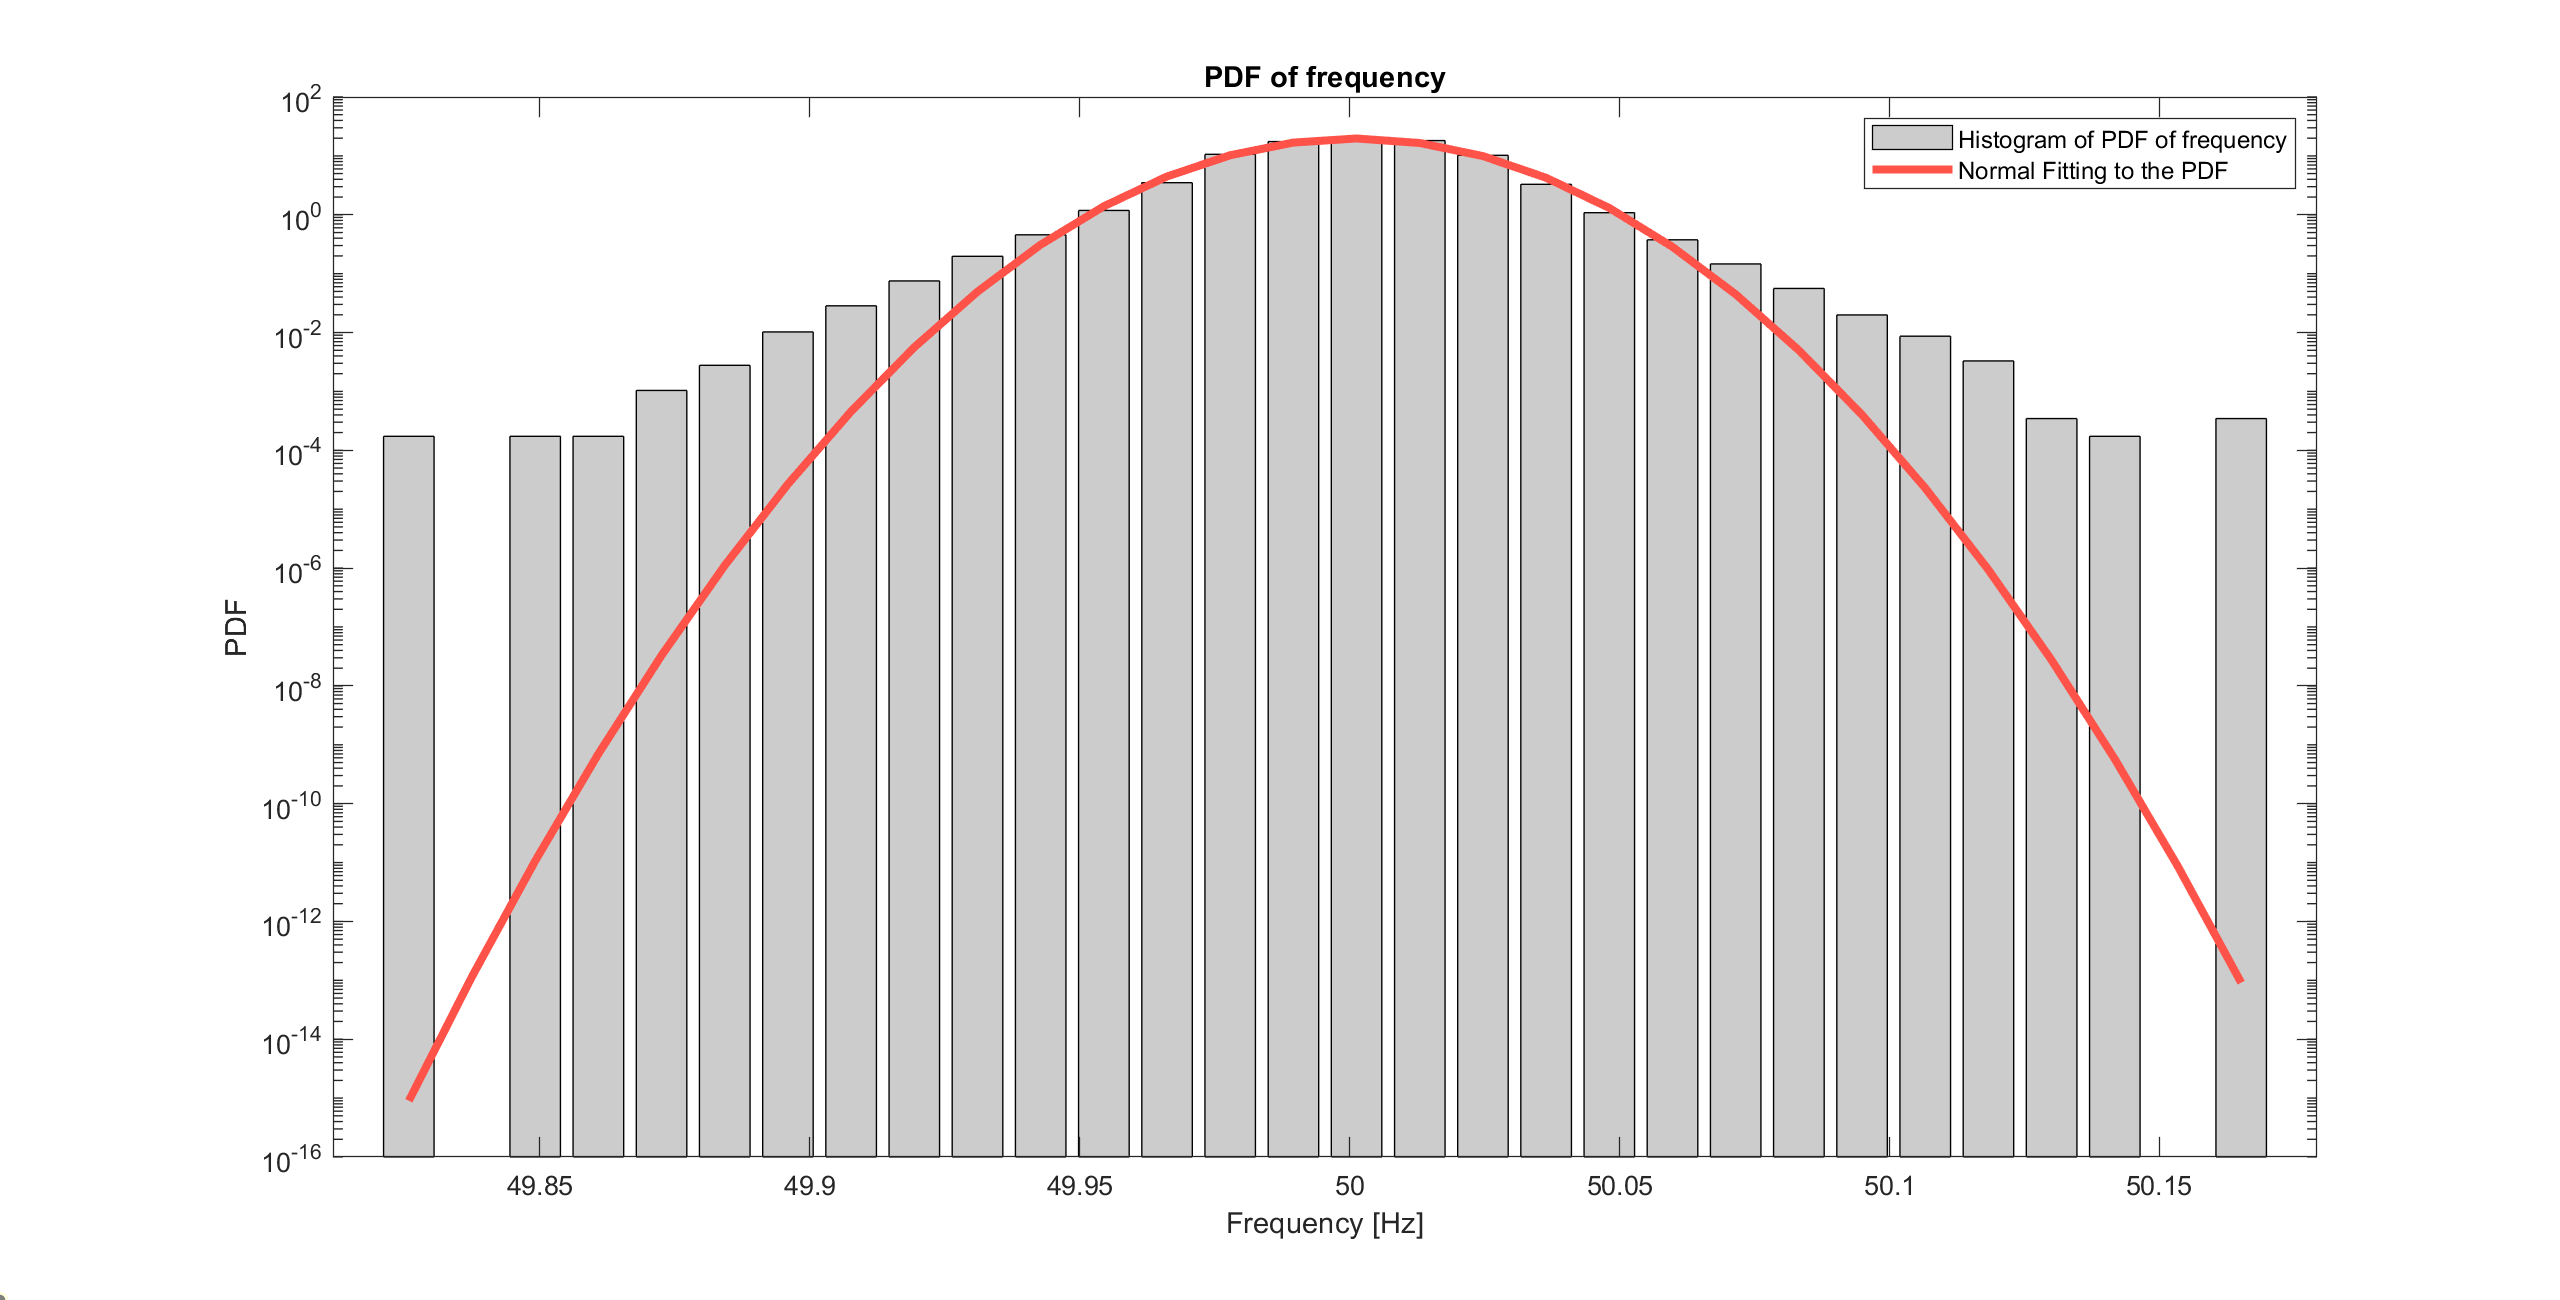
\includegraphics[scale=0.25]{../figures/pdf/pdf_frequency_continental_europe_2019}
	\caption{Frequency Probability Density Function plots for the Continental European grid for the year 2019. There is significant deviation of the actual PDF values (grey bars) from the closest Gaussian model fitted to the same data (red curve) at the tails, which are much heavier in the former.	}
\end{figure}

\begin{figure}[!ht]
	\centering
	\begin{subfigure}{\textwidth}
		\centering
		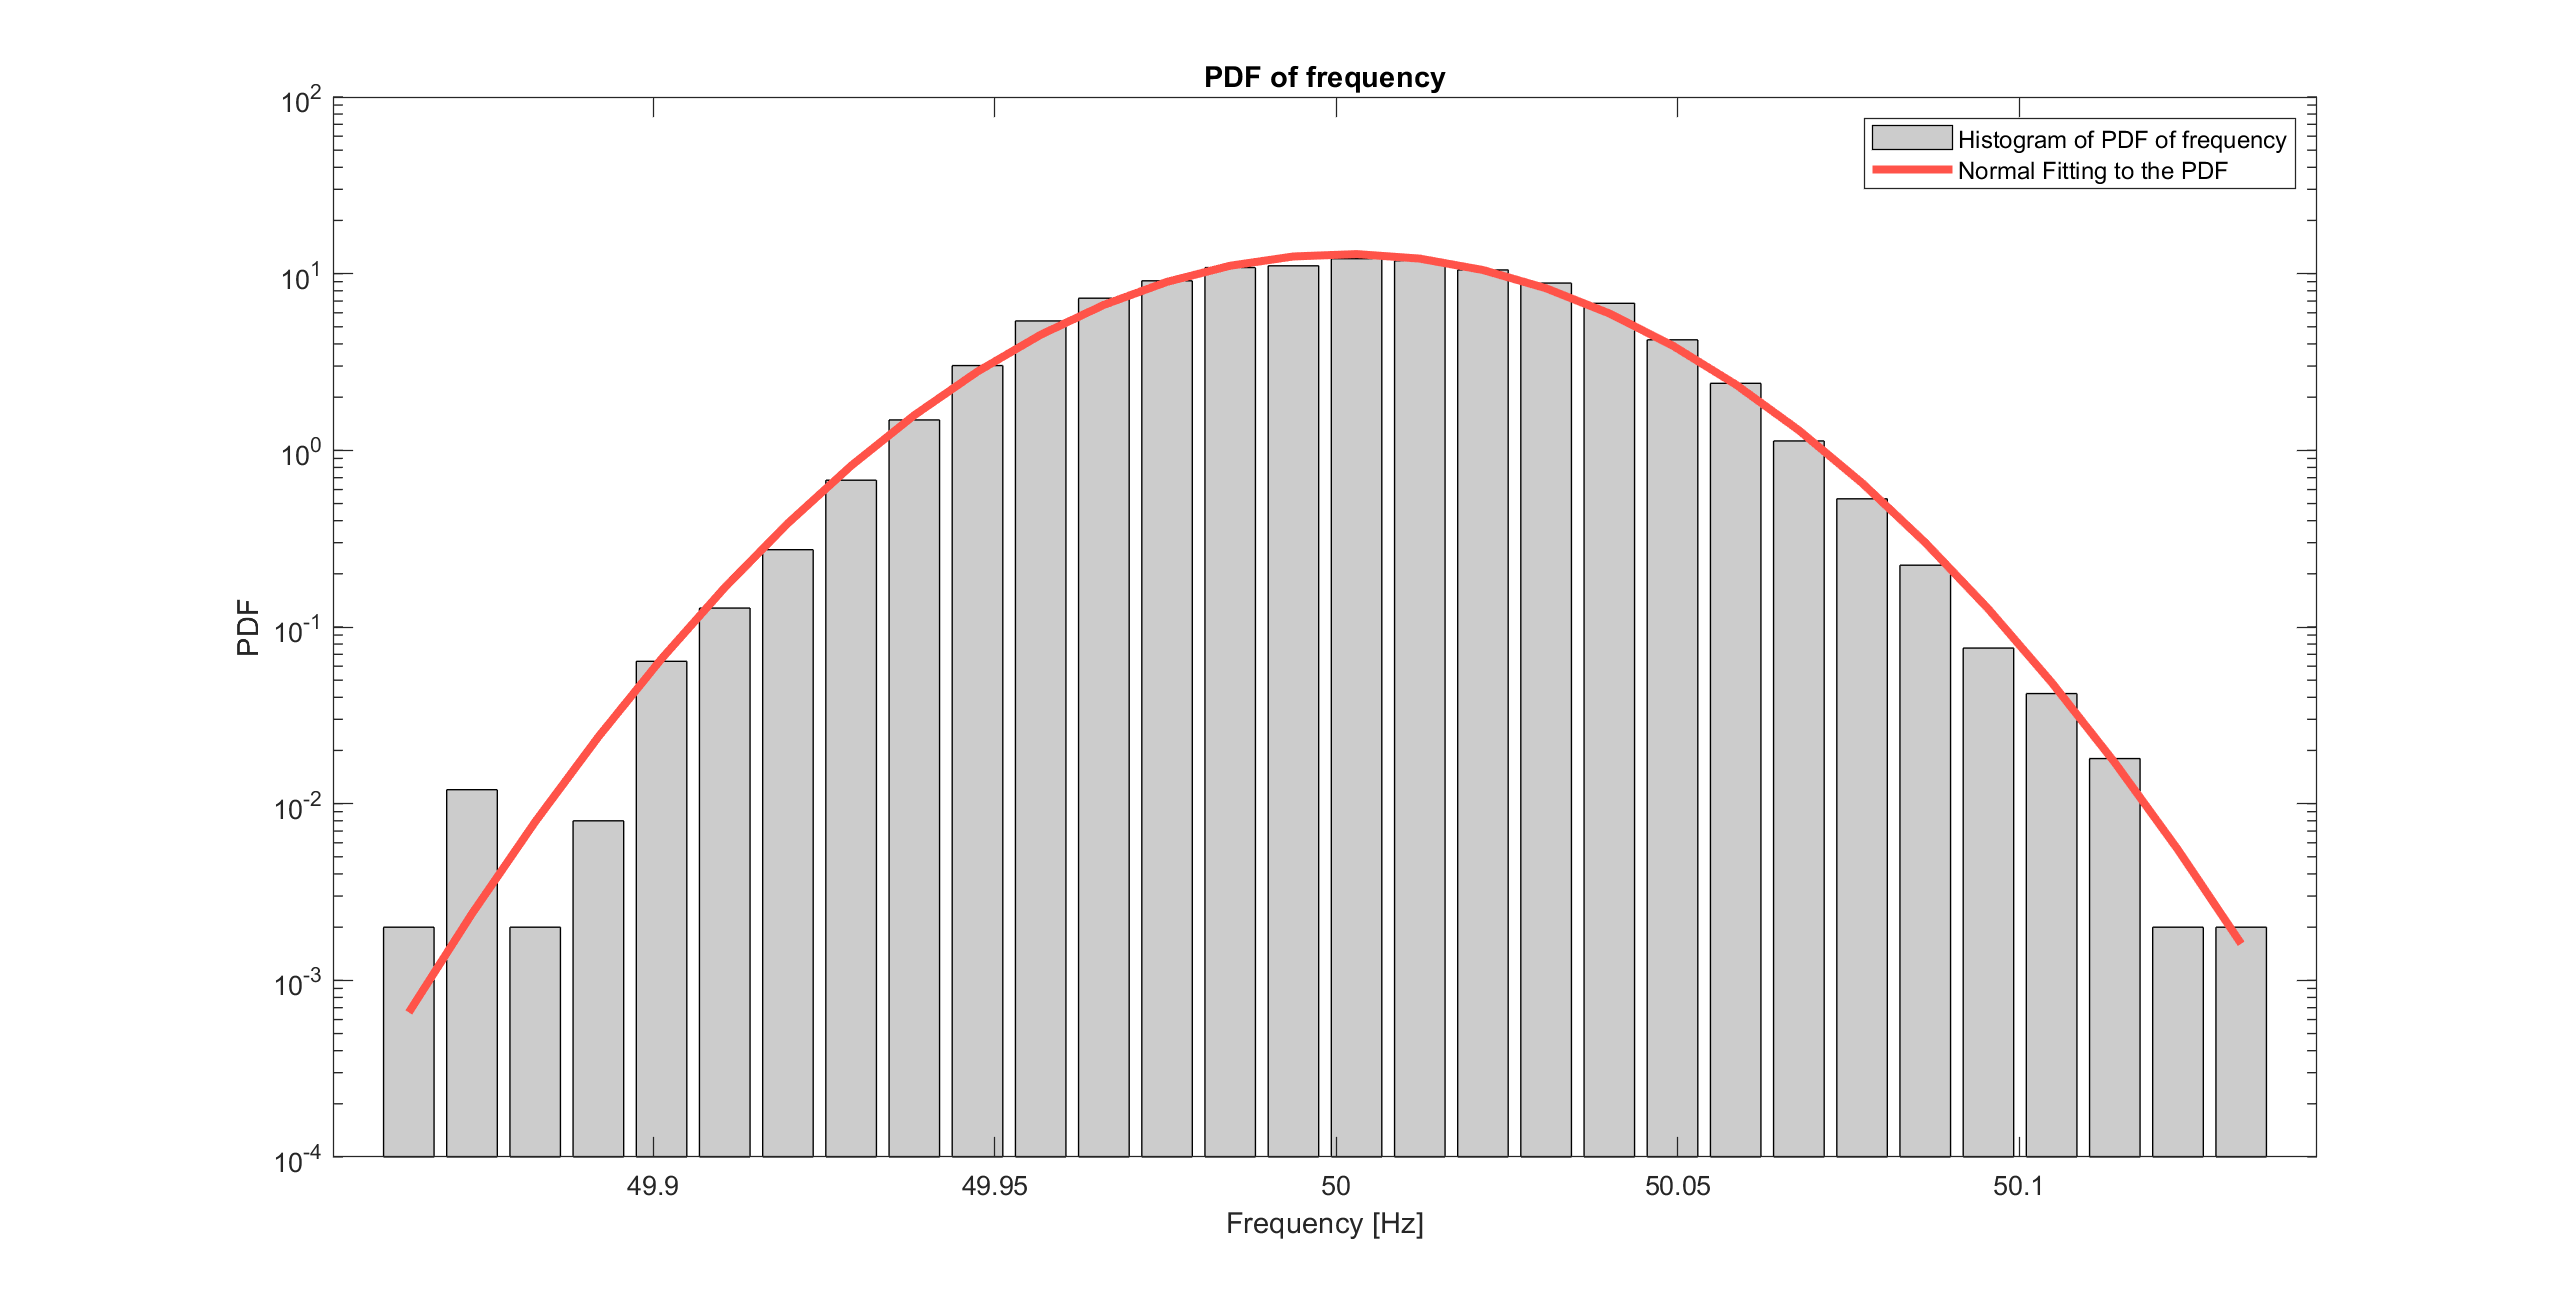
\includegraphics[scale=0.25]{../figures/pdf/pdf_frequency_tokyo_2020_01}
		\caption{Frequency Probability Density Function plots for the Tokyo grid for January 2020.}
	\end{subfigure}

	\begin{subfigure}{\textwidth}
		\centering
		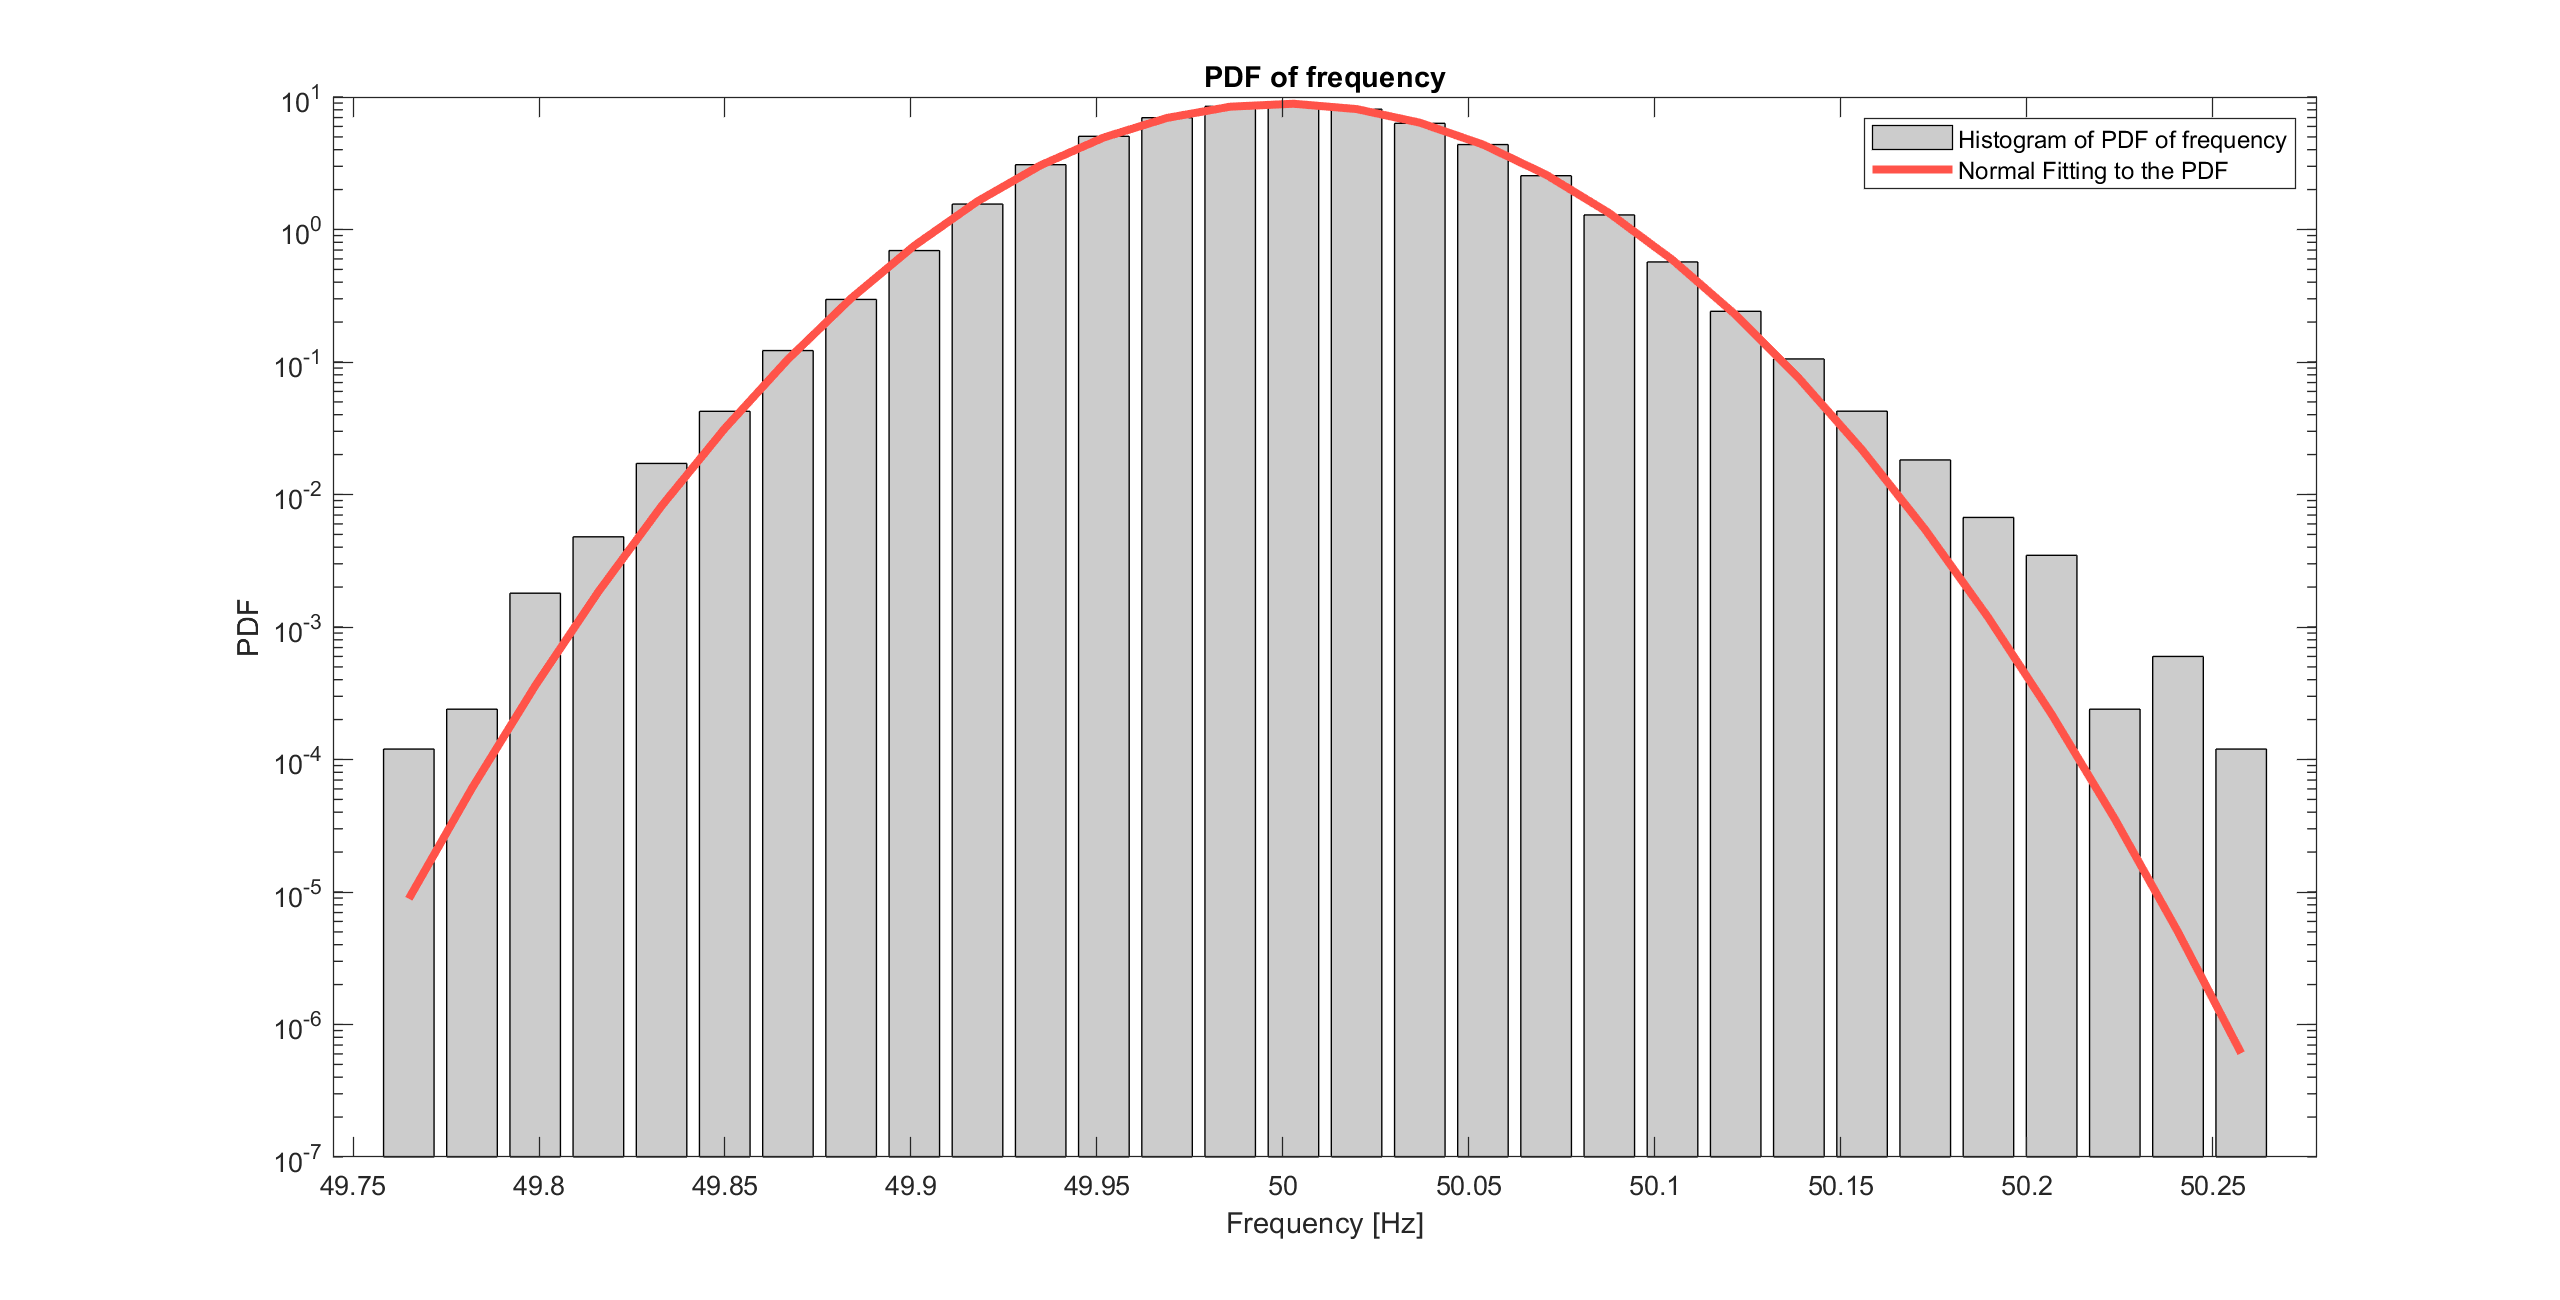
\includegraphics[scale=0.25]{../figures/pdf/pdf_frequency_nordic_2019}
		\caption{Frequency Probability Density Function plots for the Nordic grid for the year 2019.}
	\end{subfigure}
	\caption{Frequency distribution PDFs of some grids show almost identical characteristics to the Gaussian Distribution. For the case of Tokyo and Nordic grids, there is a fair level of agreement between the actual PDF values (grey bars) and the closest fitted Gaussian model (red curve). An assumption of Guassianity, for some grids, therefore is not completely unfounded.}
\end{figure}

\begin{figure}[!ht]
	\centering
	\begin{subfigure}{\textwidth}
		\centering
		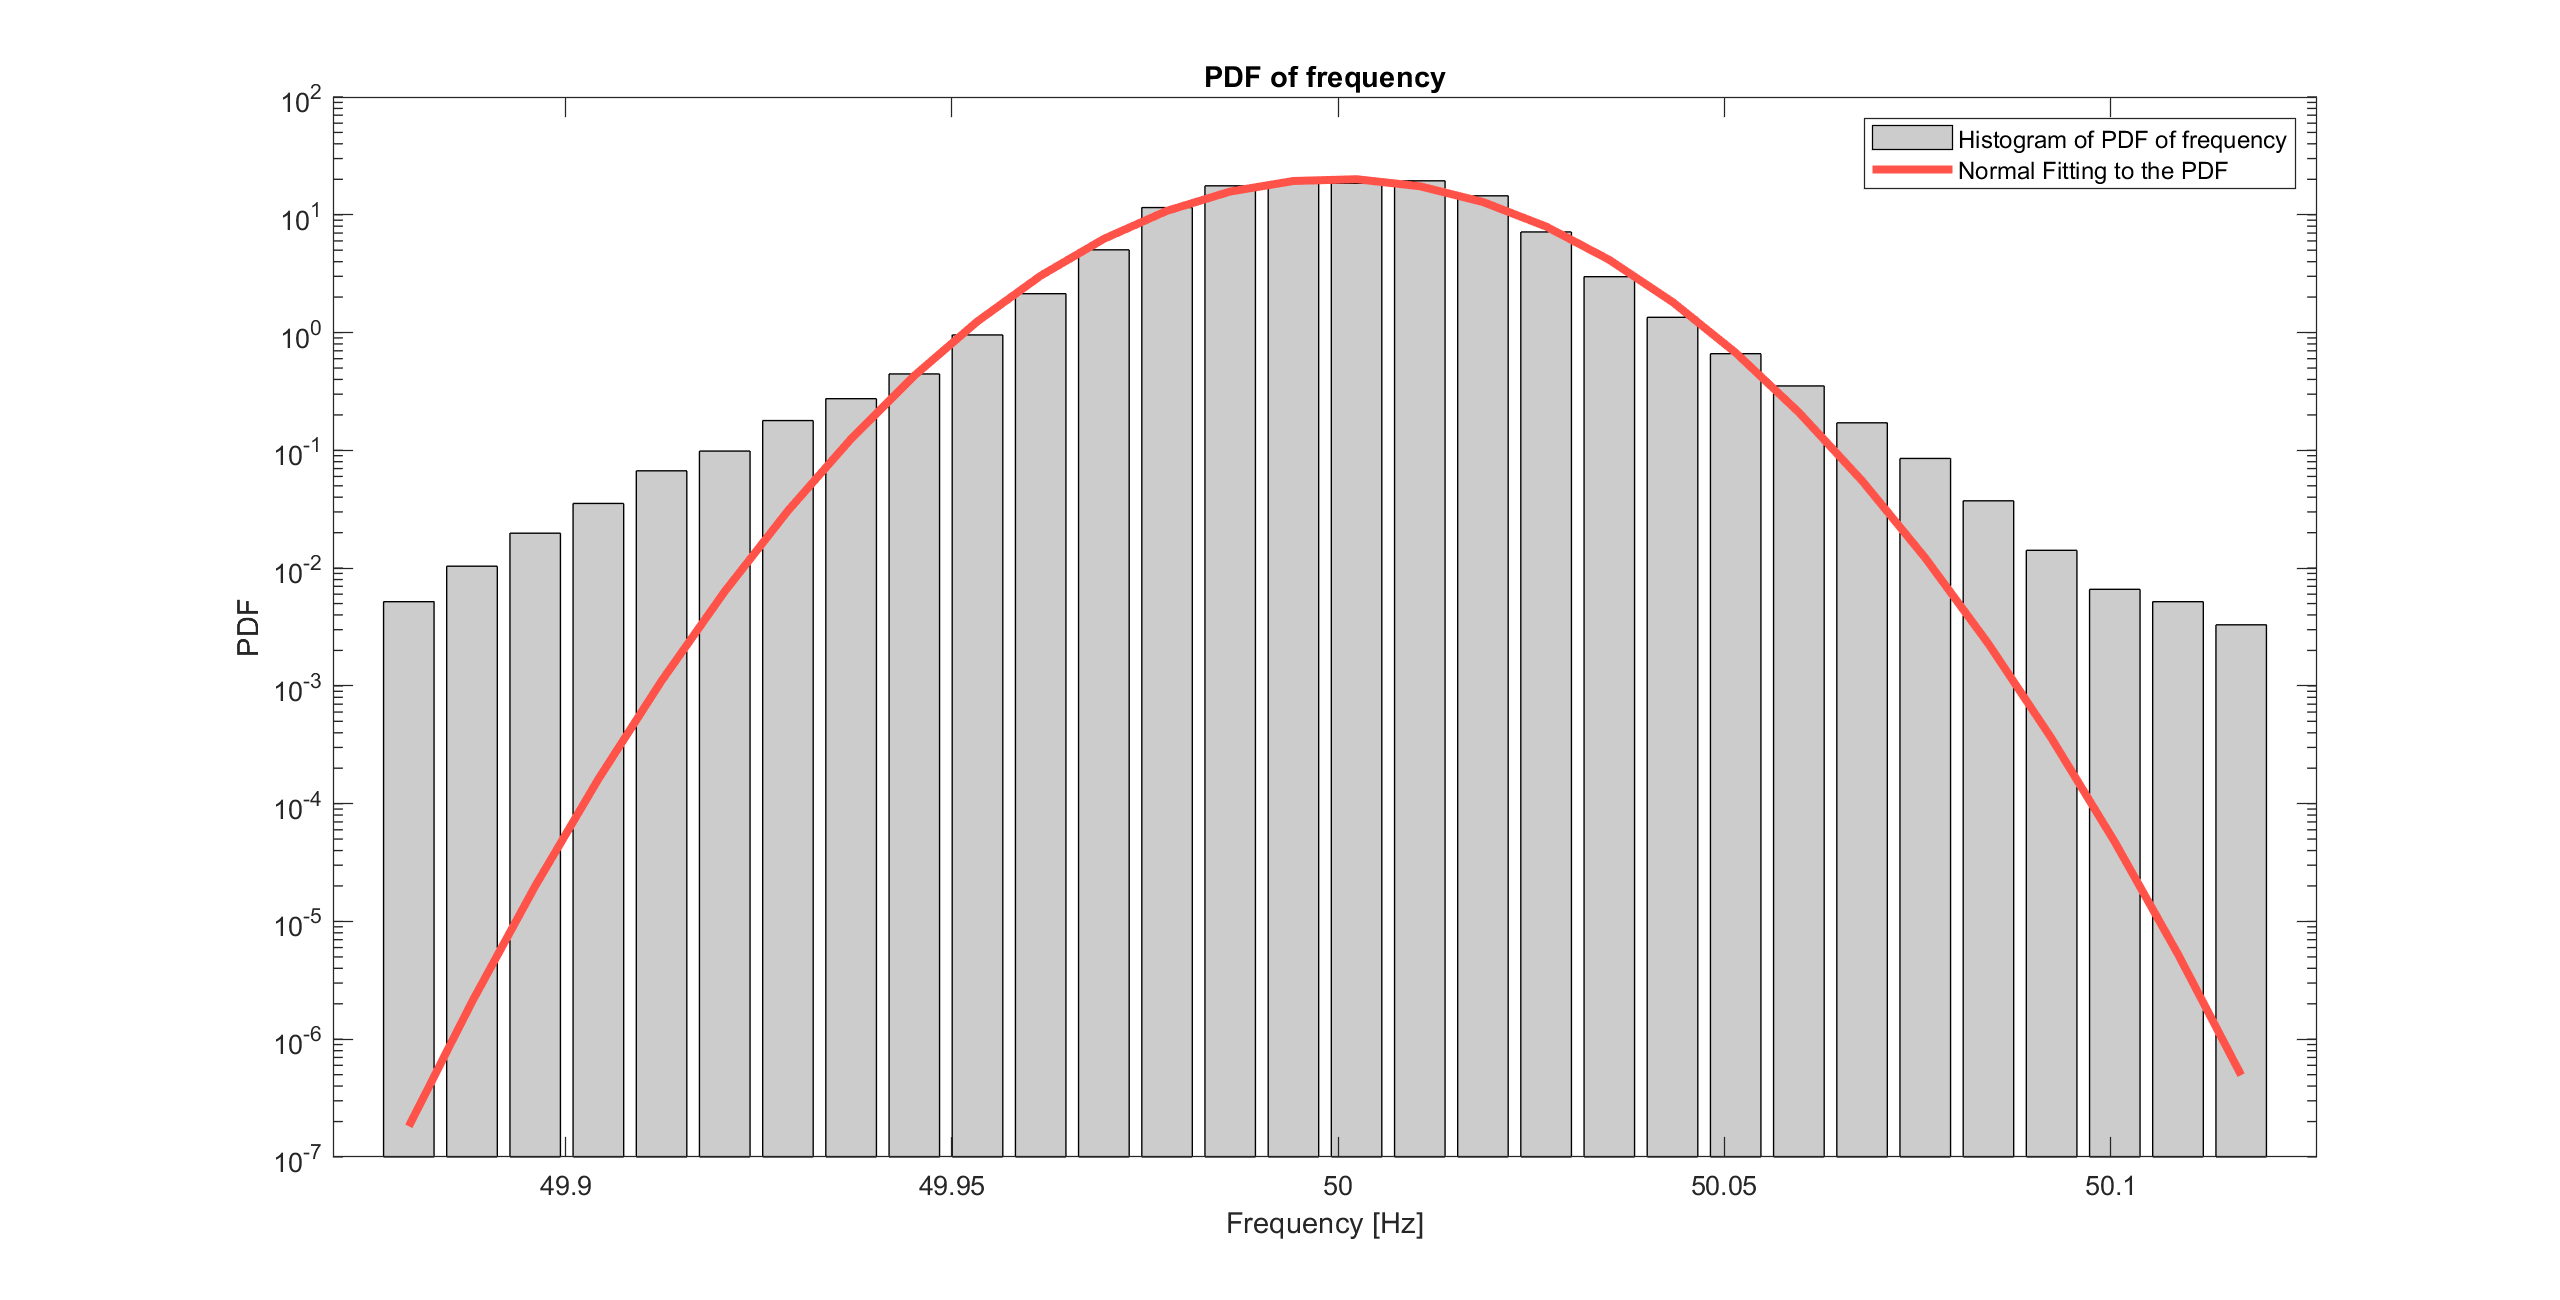
\includegraphics[scale=0.25]{../figures/pdf/pdf_frequency_rte_2019_09}
		\caption{Frequency Probability Density Function plot for the French RTE grid for September 2019.}
	\end{subfigure}
	
	\begin{subfigure}{\textwidth}
		\centering
		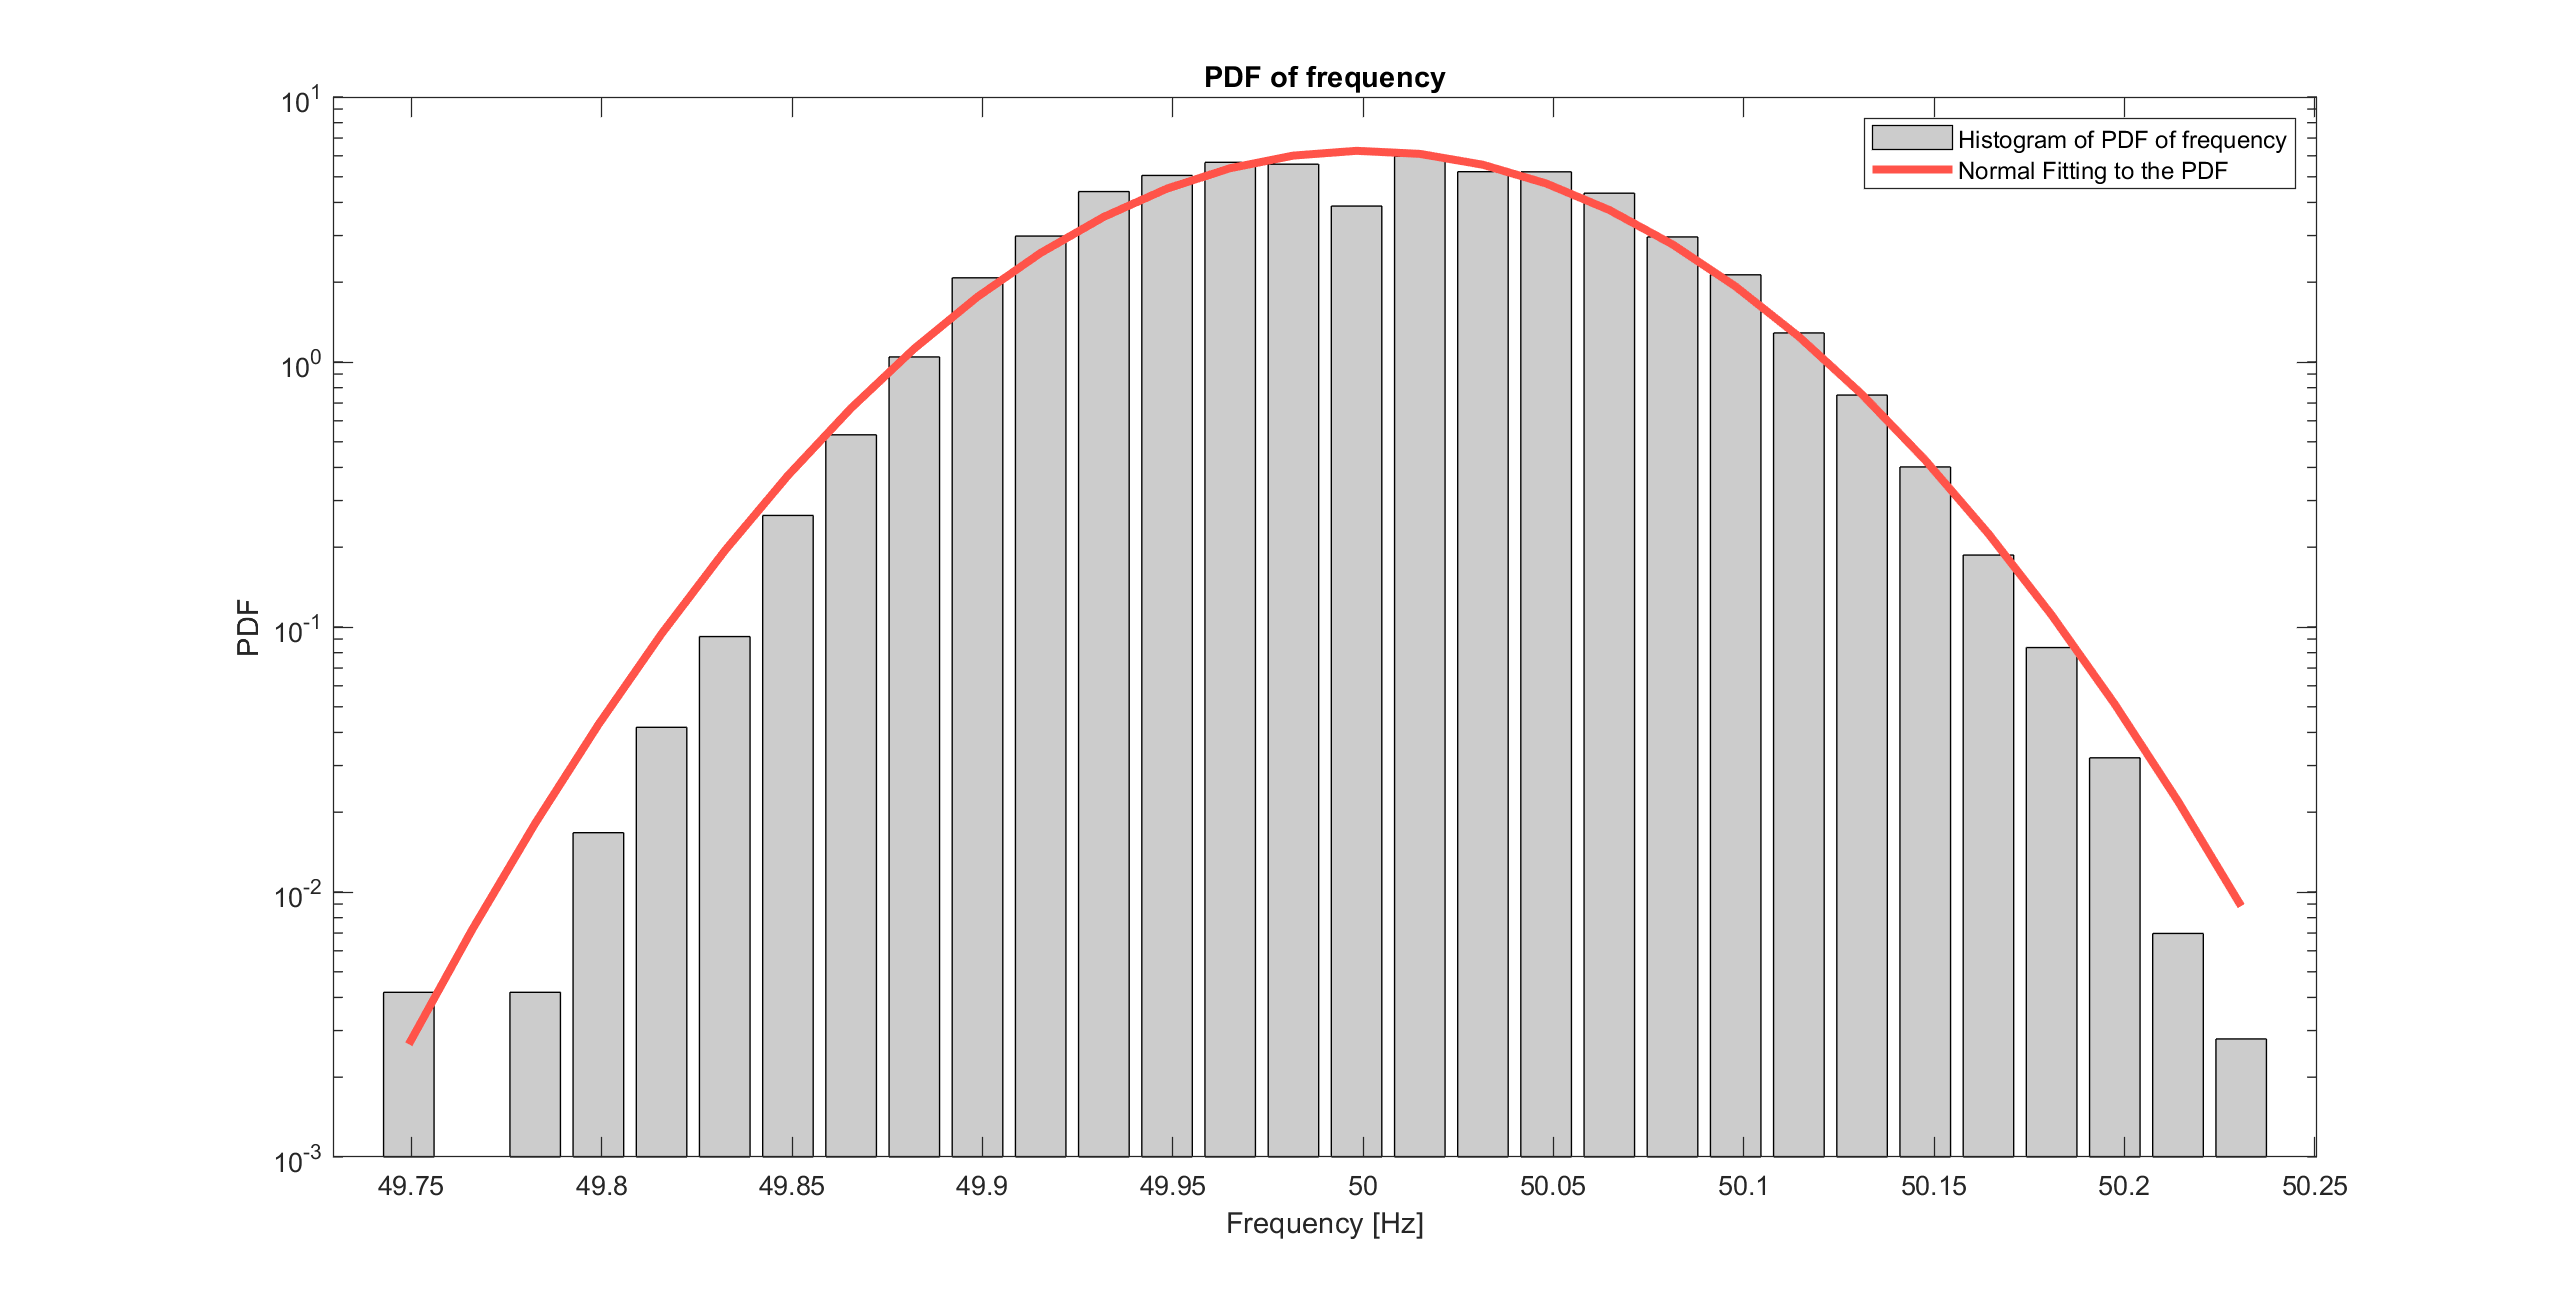
\includegraphics[scale=0.25]{../figures/pdf/pdf_frequency_uk_2020_04}
		\caption{Frequency Probability Density Function plot for the Great Britain grid for April 2020.}
	\end{subfigure}

	\caption{Some sets of grids show an appreciable level of deviation from the Gaussian distribution in that: they have heavier tails, such as for the French RTE Grid, or they have a bimodal distribution (two peaks), such as for the Great Britain Grid.}
\end{figure}

\begin{figure}[!ht]
	\centering
	\begin{subfigure}{\textwidth}
		\centering
		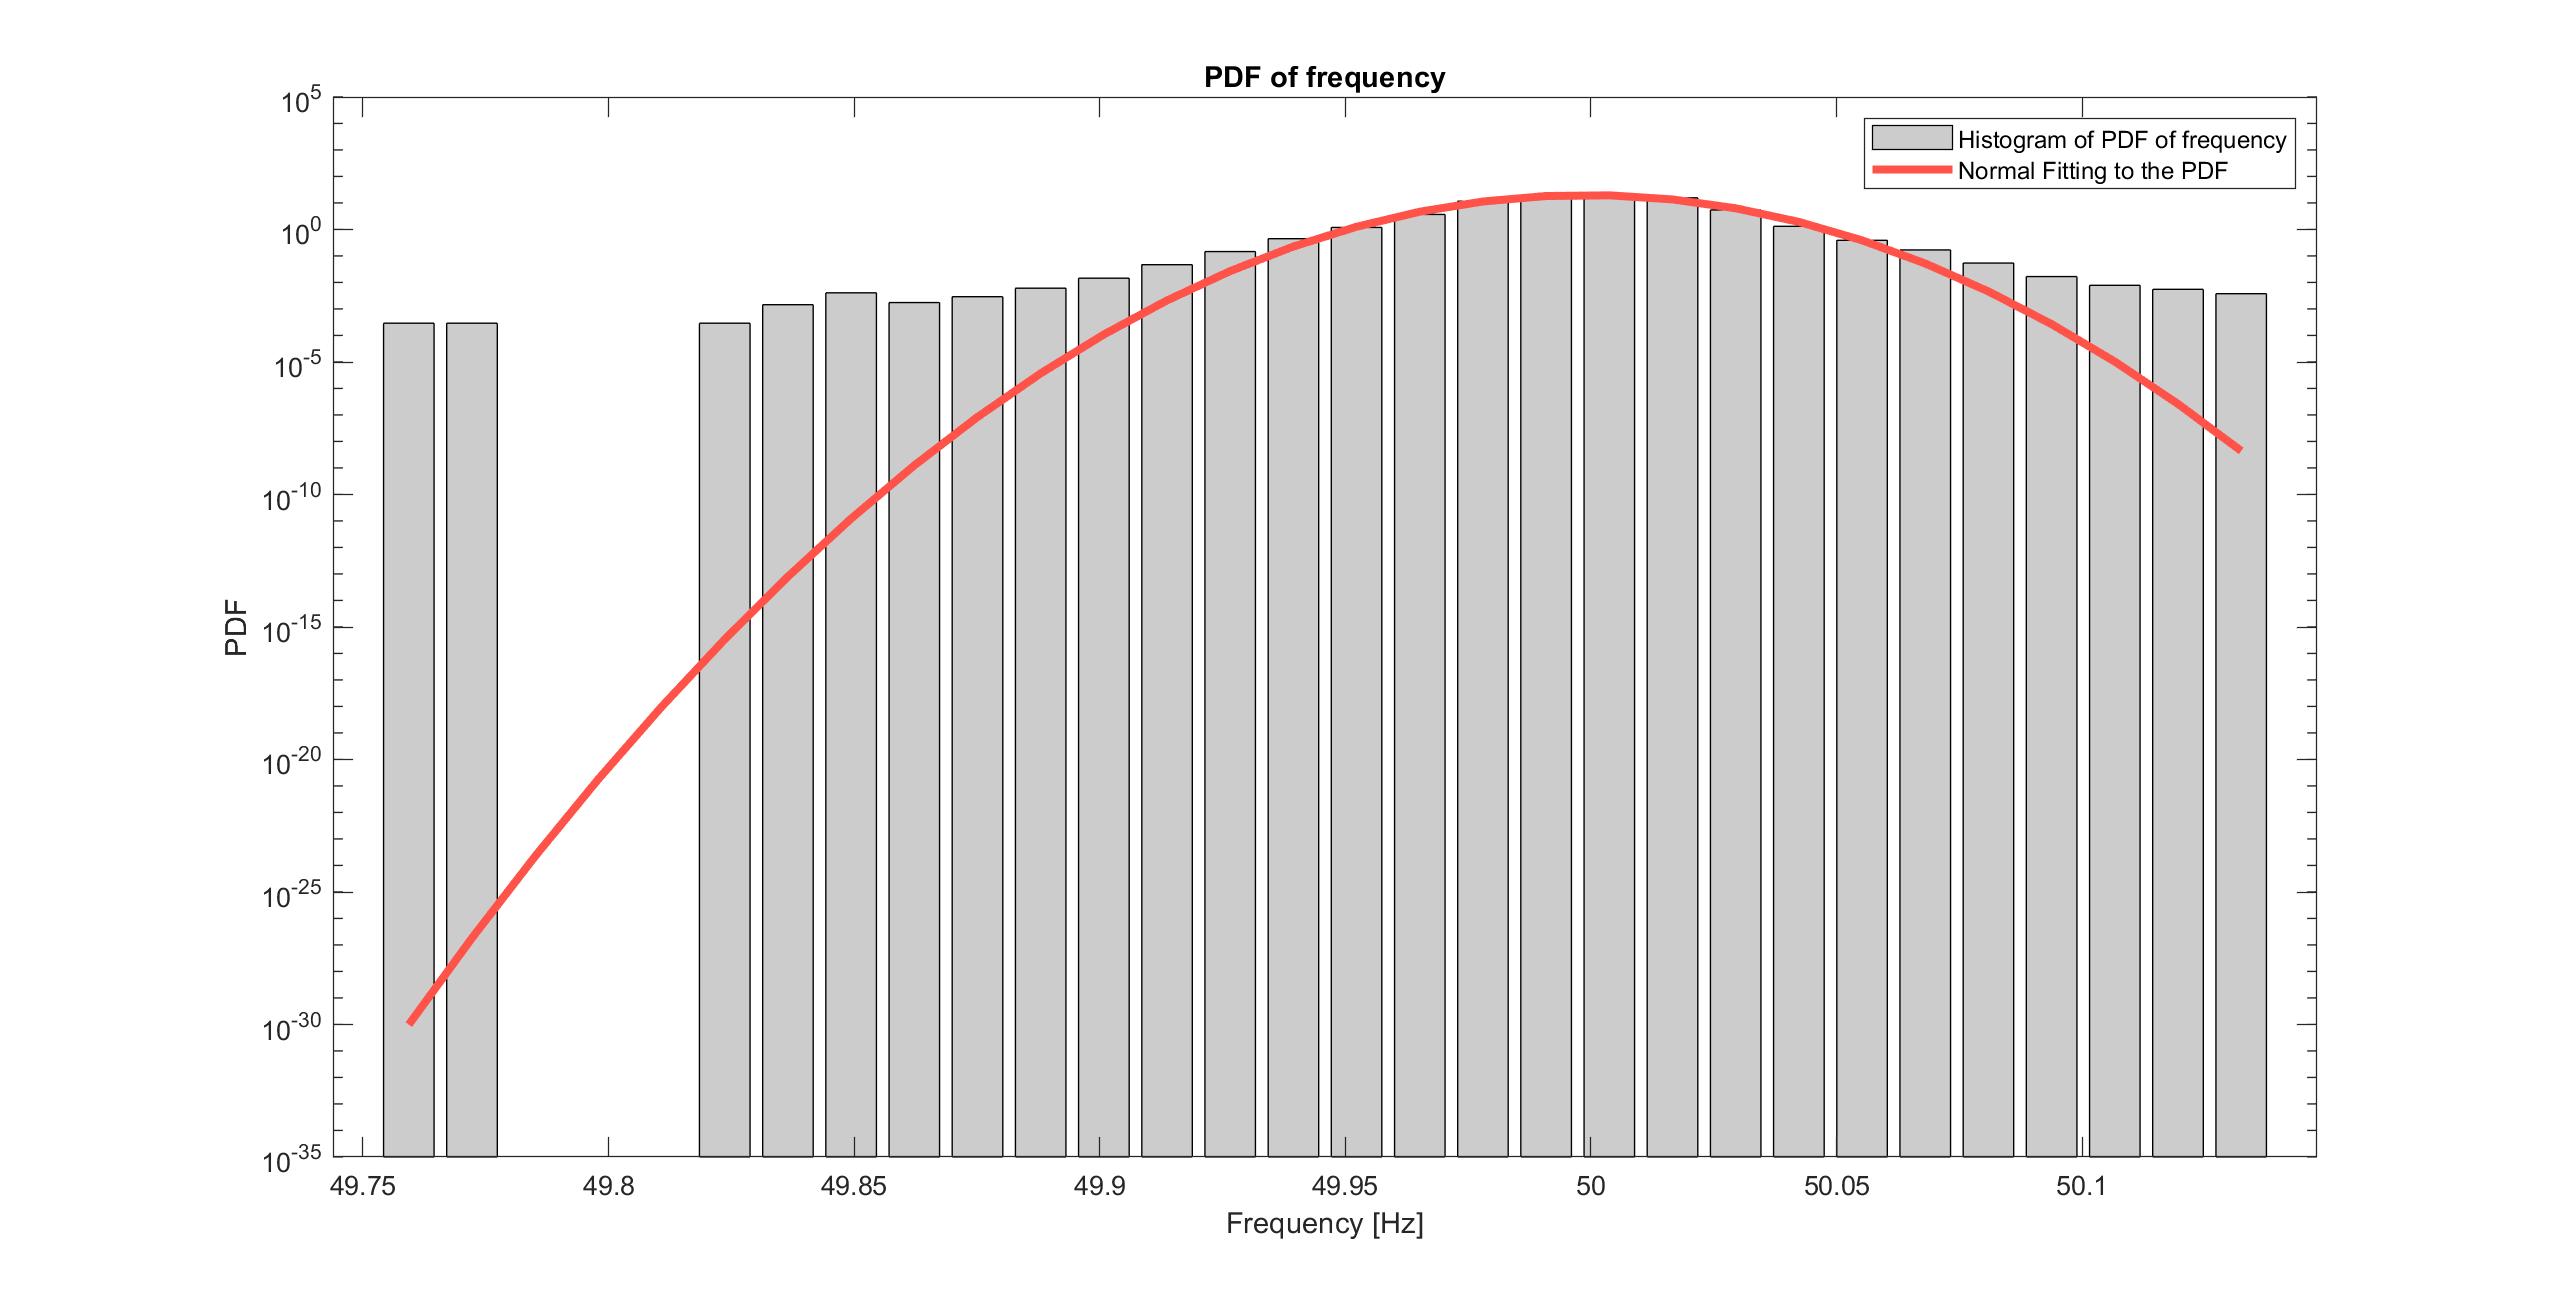
\includegraphics[scale=0.25]{../figures/pdf/pdf_frequency_rte_2021_01_blackout}
		\caption{Frequency Probability Density Function plot for the French RTE grid for January 2021.}
	\end{subfigure}
	
	\begin{subfigure}{\textwidth}
		\centering
		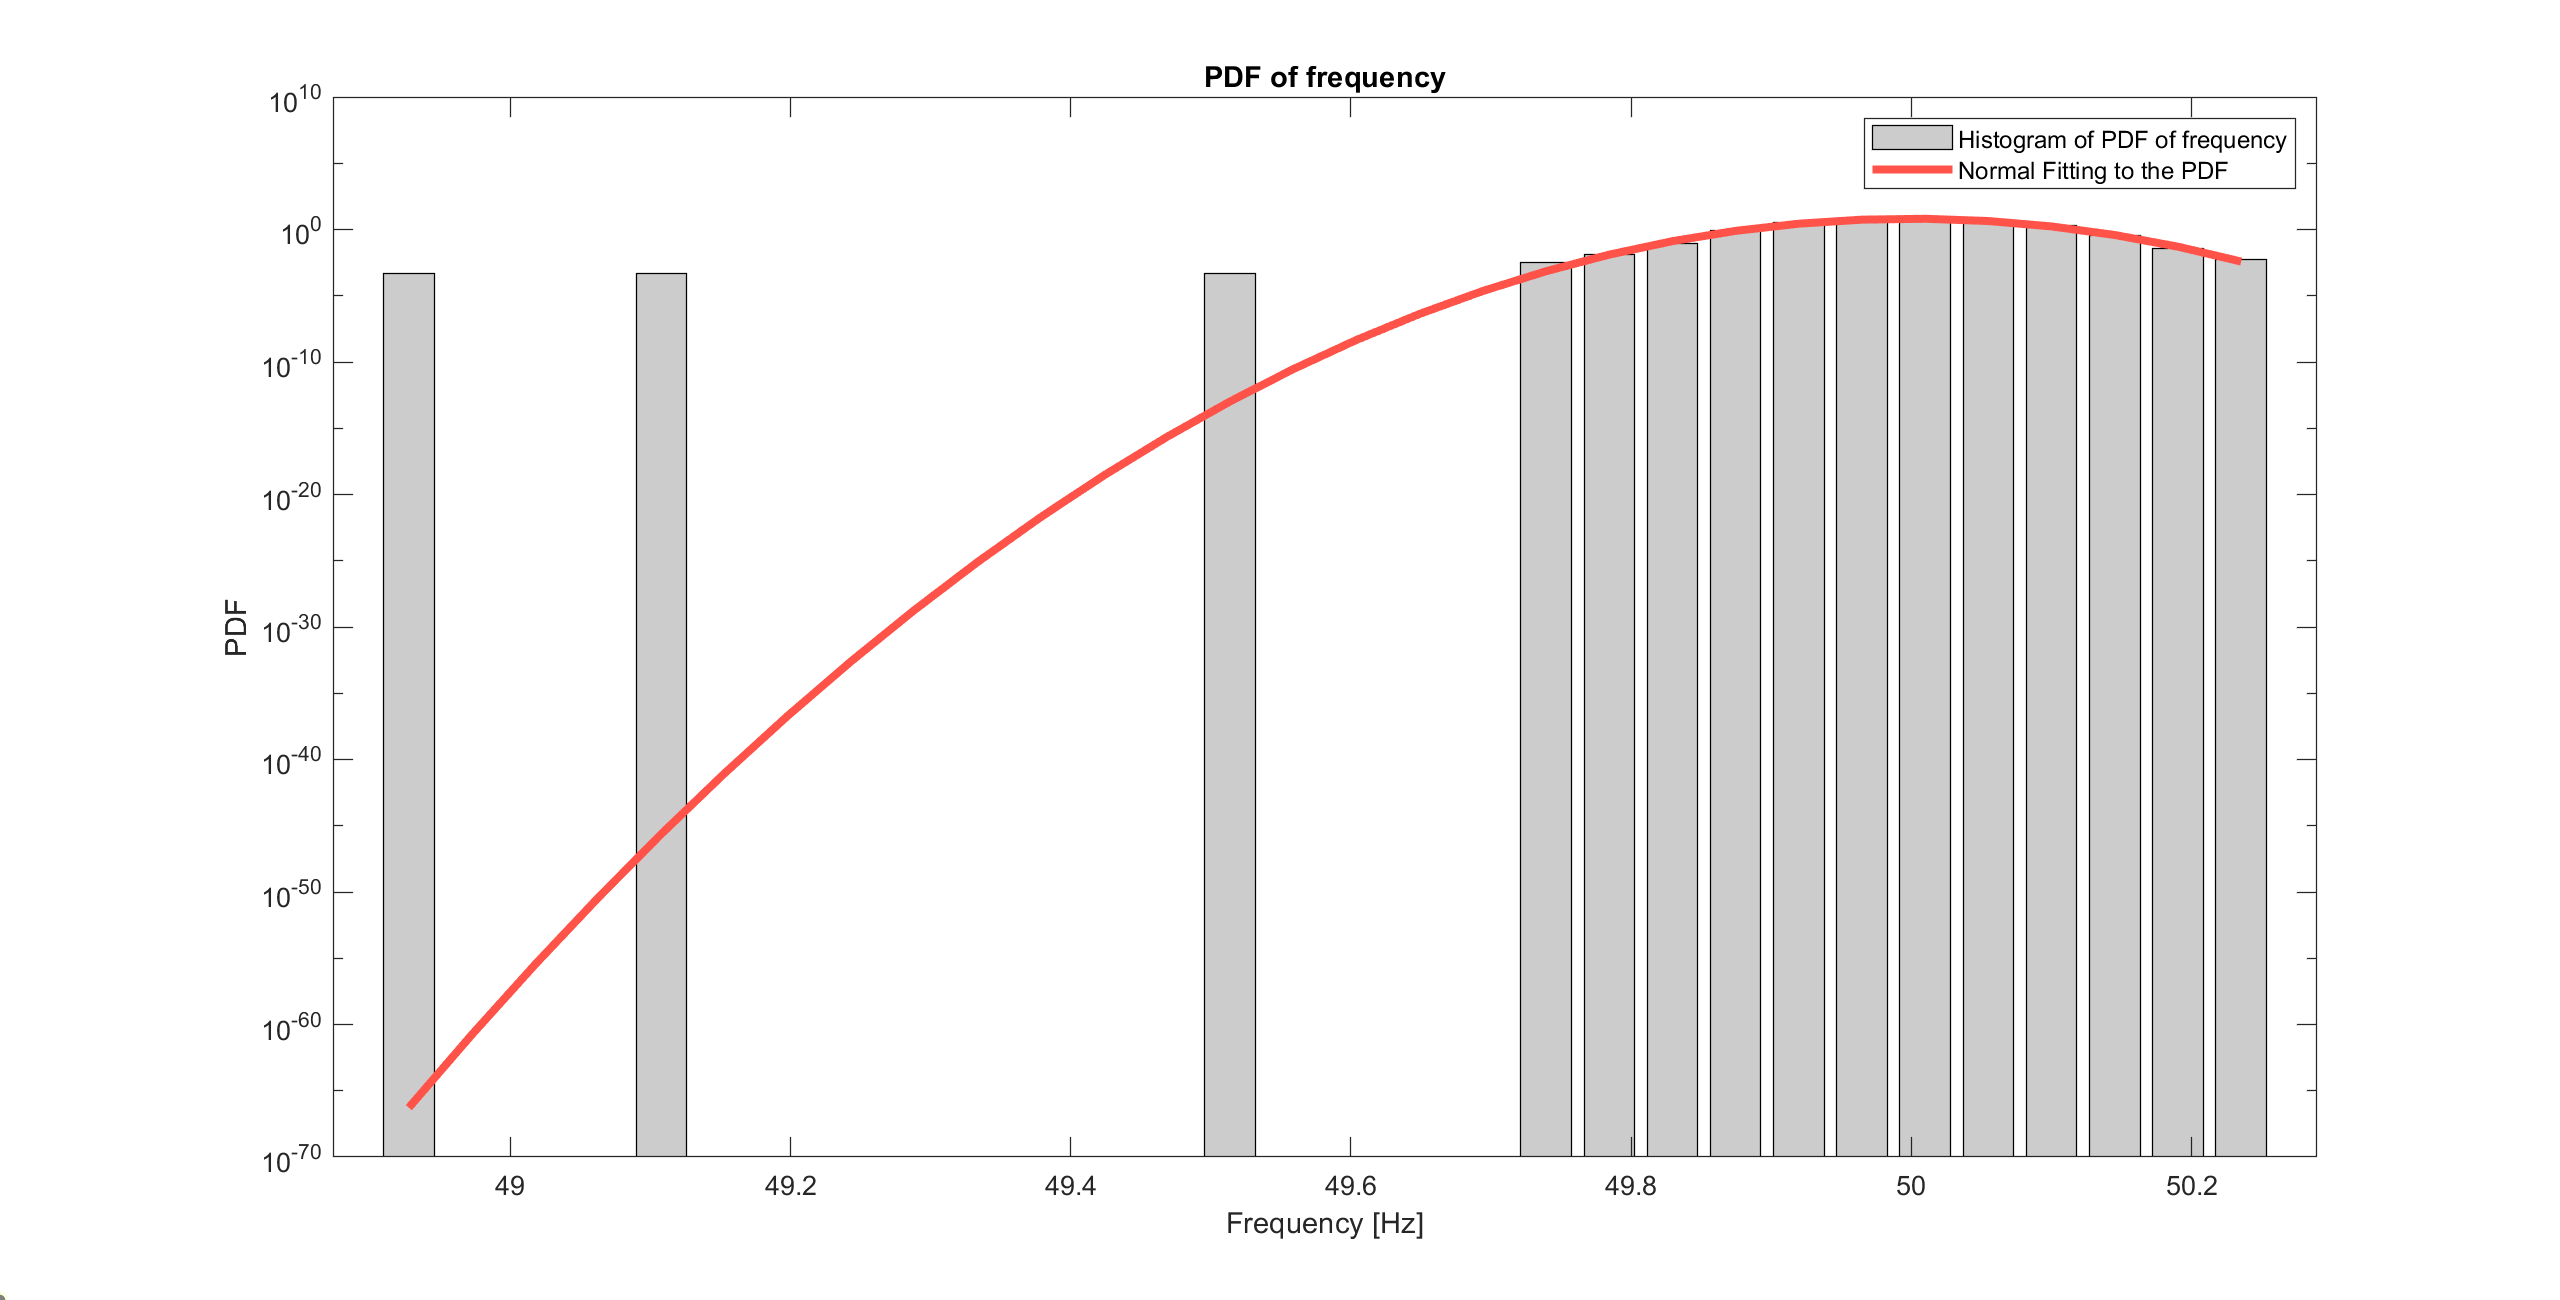
\includegraphics[scale=0.25]{../figures/pdf/pdf_frequency_uk_2019_08_blackout}
		\caption{Frequency Probability Density Function plot for the Great Britain grid for August 2019.}
	\end{subfigure}
	\caption{Blackouts are easily singled out in visual post mortem analysis of grid frequency PDFs. A frequency PDF of a grid plotted for a time duration incorporating a blackout is generally too anomalous from the `usual' non-blackout PDFs. In the above plots, the severe outliers in the PDFs of the French RTE and the Great Britain grids were the results of occurrence of a 10 minute blackout on 08 January 2021 and a 5 minute blackout on 09 August 2019 respectively.}
\end{figure}

\begin{figure}[!ht]
	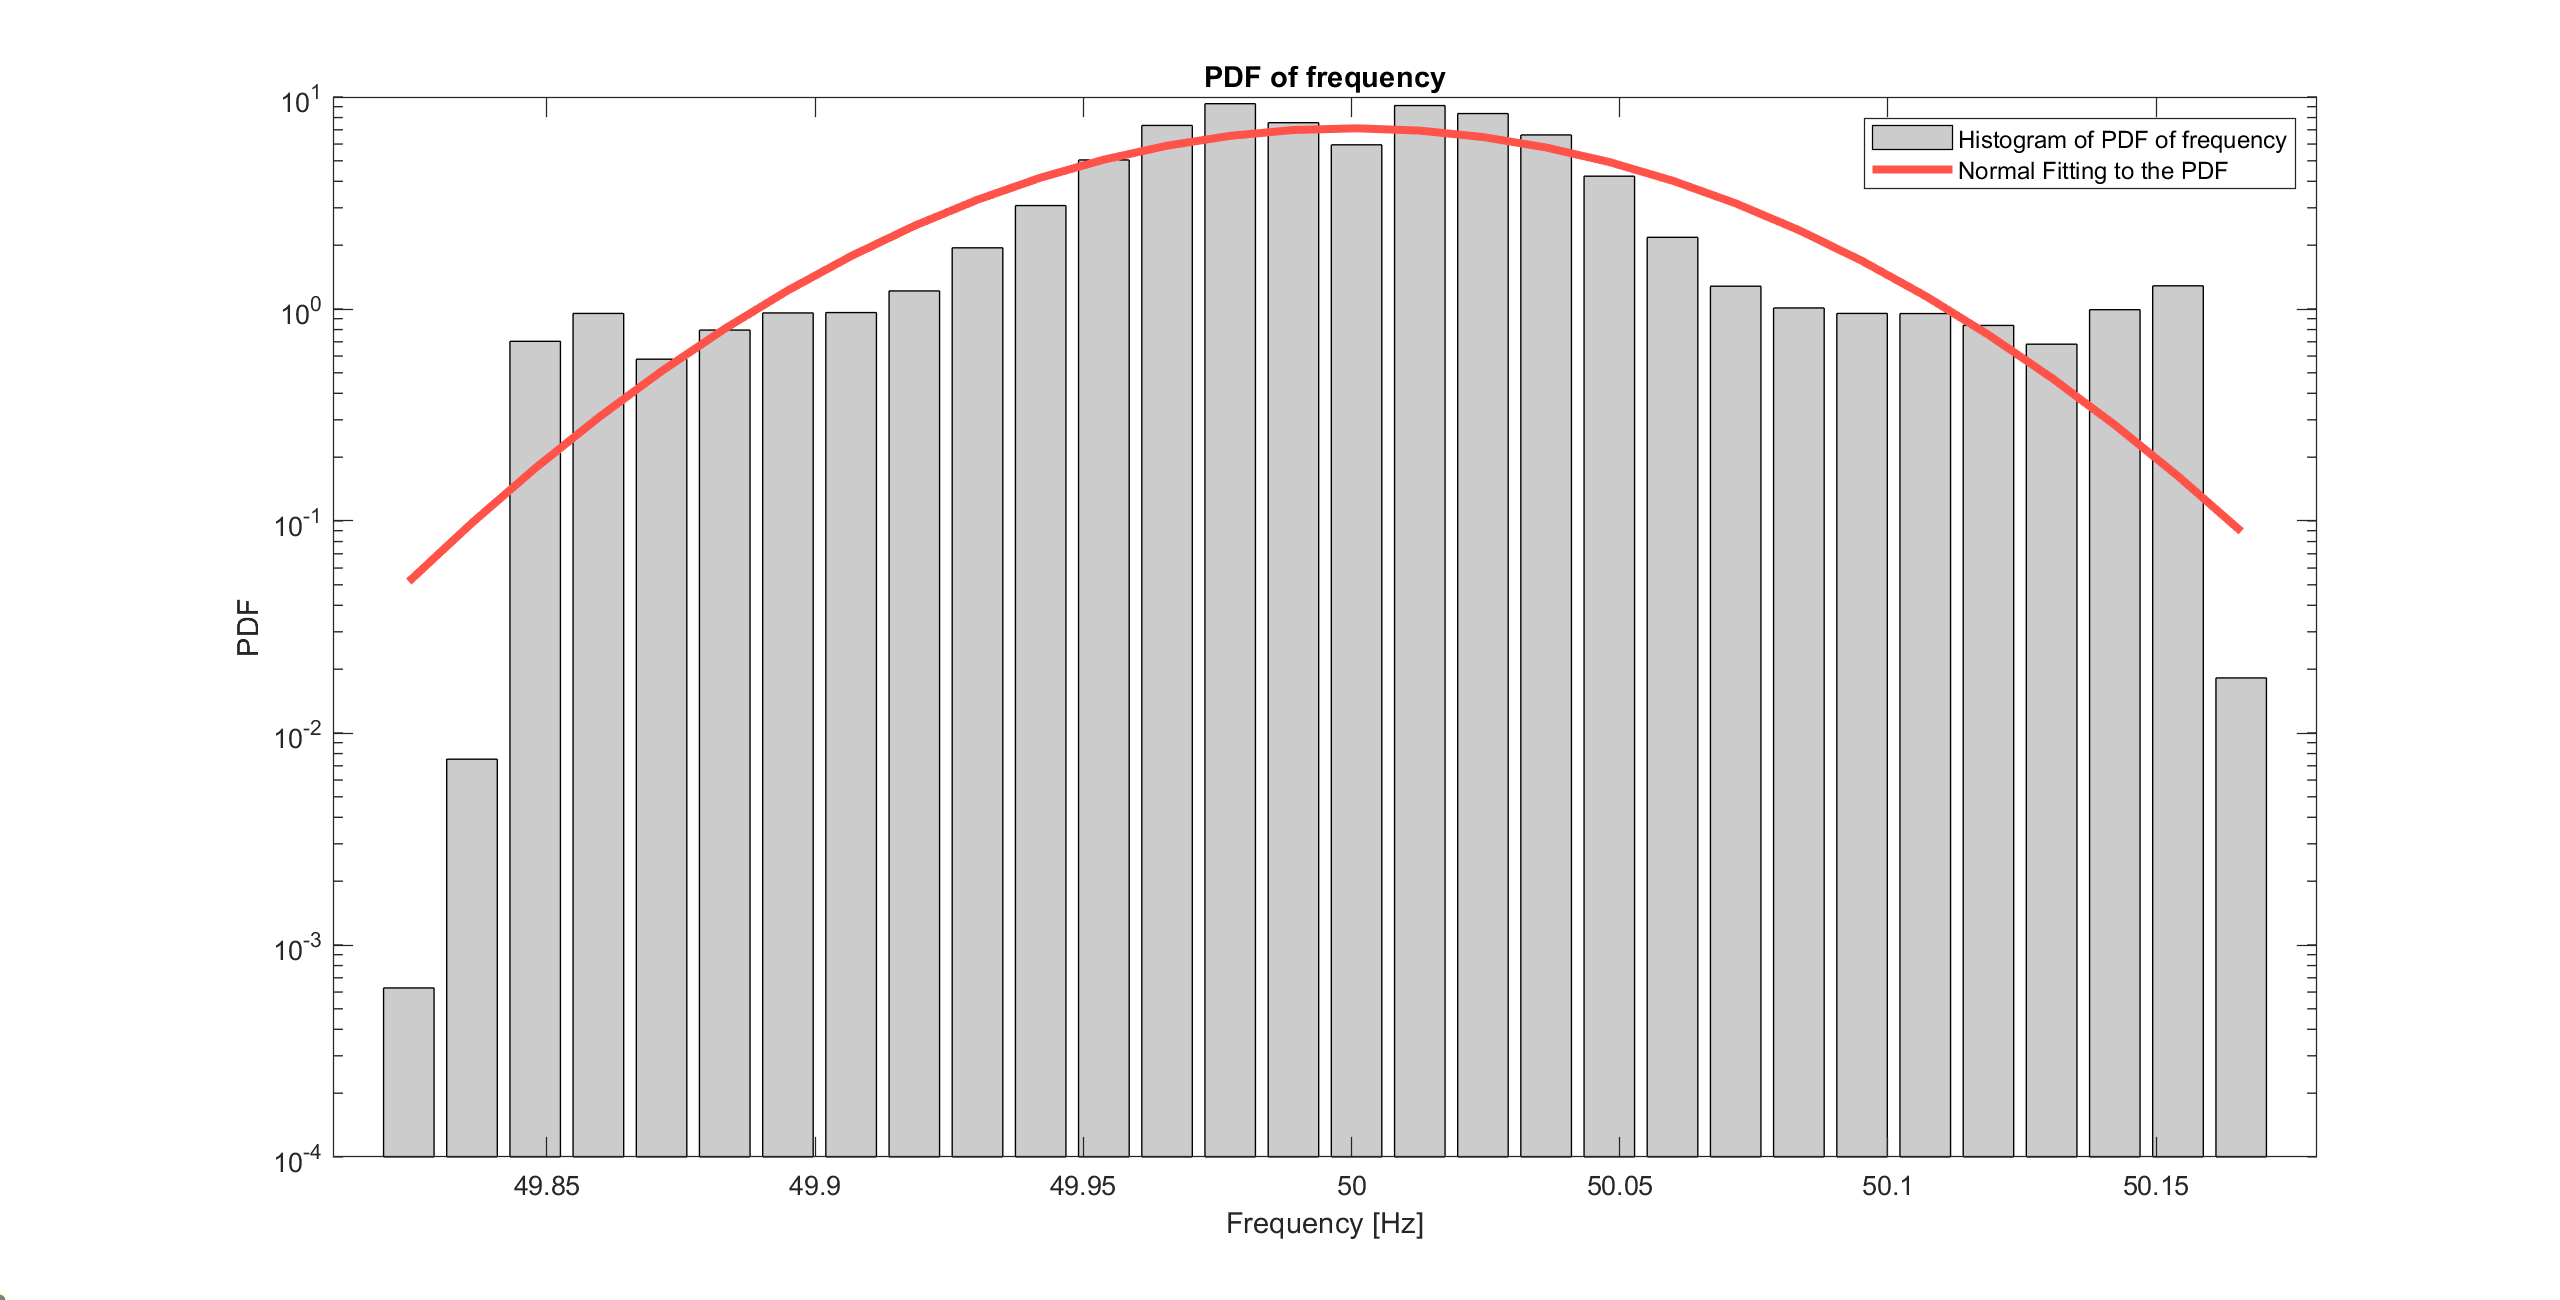
\includegraphics[scale=0.25]{../figures/pdf/pdf_frequency_spain_mallorca_2019_05_f1}
	\caption{Frequency Probability Density Function plots for the Spanish Mallorcan grid for the May 2019. There is high degree of deviation of the actual PDF values (grey bars) from the closest Gaussian model fitted to the same data (red curve). Apart from the heavier tails, the frequency distribution appears to have multiple peaks.}
\end{figure}


The plotted bulk distribution PDFs visually revealed insights including any deadbands \cite{francesca01, vorobev01} mandated in their grid operation, their skewness, thickness of their tails, etc. A quantitative study of their moments like kurtosis and skewness was not conducted as was done in \cite{schafer01}.

\begin{figure}[ht]
	\centering
	\resizebox{0.75\linewidth}{!}{\import{../figures/autocorr}{comparison_five_no_title.tex}}
	\caption{Fixed Time Autocorrelation plots for five different power grids. The different rates of exponential decay in autocorrelation values indicates the difference in their relative damping strengths. The Continental European and Great Britain grids display peaks every $15$ minutes which may be explained from their energy dispatch routine.}
	\label{fig:comp5}
\end{figure}

In the plotted autocorrelation decay curves, all grids showed exponentially decreasing autocorrelations $c(\tau$) for smaller values of $\tau$. In order to confirm if the decrease was indeed exponential with a grid-specific decay constant also called as the inverse-time correlation or ${t_{corr}}^{-1}$, semi-log graphs ($\log(c(\tau))$ vs $\tau$) were also plotted. The decay constants were computed by calculating the slopes of the semi-log graphs and it was found that the grids which were bigger, more robust and showed bulk distribution PDFs which were less-deviating from Gaussian distributions, had greater values of inverse-time correlation ${t_{corr}}^{-1}$. This parameter can also be construed as $\alpha$, the relative damping strength of the grid for small oscillations and can be an indicator of the overall robustness of the grid.

\subsection*{Effect of sampling duration on consistency of offline analysis of data}
\label{app:effectOfSamplingDuration}

Different grids can have their own set of `events', such as firing up of boilers or other kinds of switching events, or `cycles' of changes, such as sub-hourly power dispatches, semi-diurnal variation in solar generation, hourly wind power fluctuations, etc. A question then arises: Can the `statistical nature' of a grid be really generalized if it itself doesn't show a constant characteristic in its dynamics? The answer is: Yes, but only if a `sufficient' duration of data has been collected for analysis, such that all kinds of cyclical variations are `averaged-out' over the duration, displaying a somewhat consistent statistical signature irrespective of the actual time the analysis was made or data collected from.

Data for different years or months of select grids (Great Britain, France RTE, Nordic, Japan) mentioned in Table \ref{tab:realGridSamplingData} were compared in terms of their Fixed Time Autocorrelation plots (Autocorrelation Decay Curves). The plots were a mixture of year-wise (Nordic), month-wise (Great Britain, France RTE, Tokyo) and day-wise (Indian NRLDC) data. It was concluded that, barring some small vertical shifts among the autocorrelation values, the trends were consistently displayed for year-wise and month-wise plots, but did not show consistency in their day-to-day plots. 

\begin{figure}[!ht]
	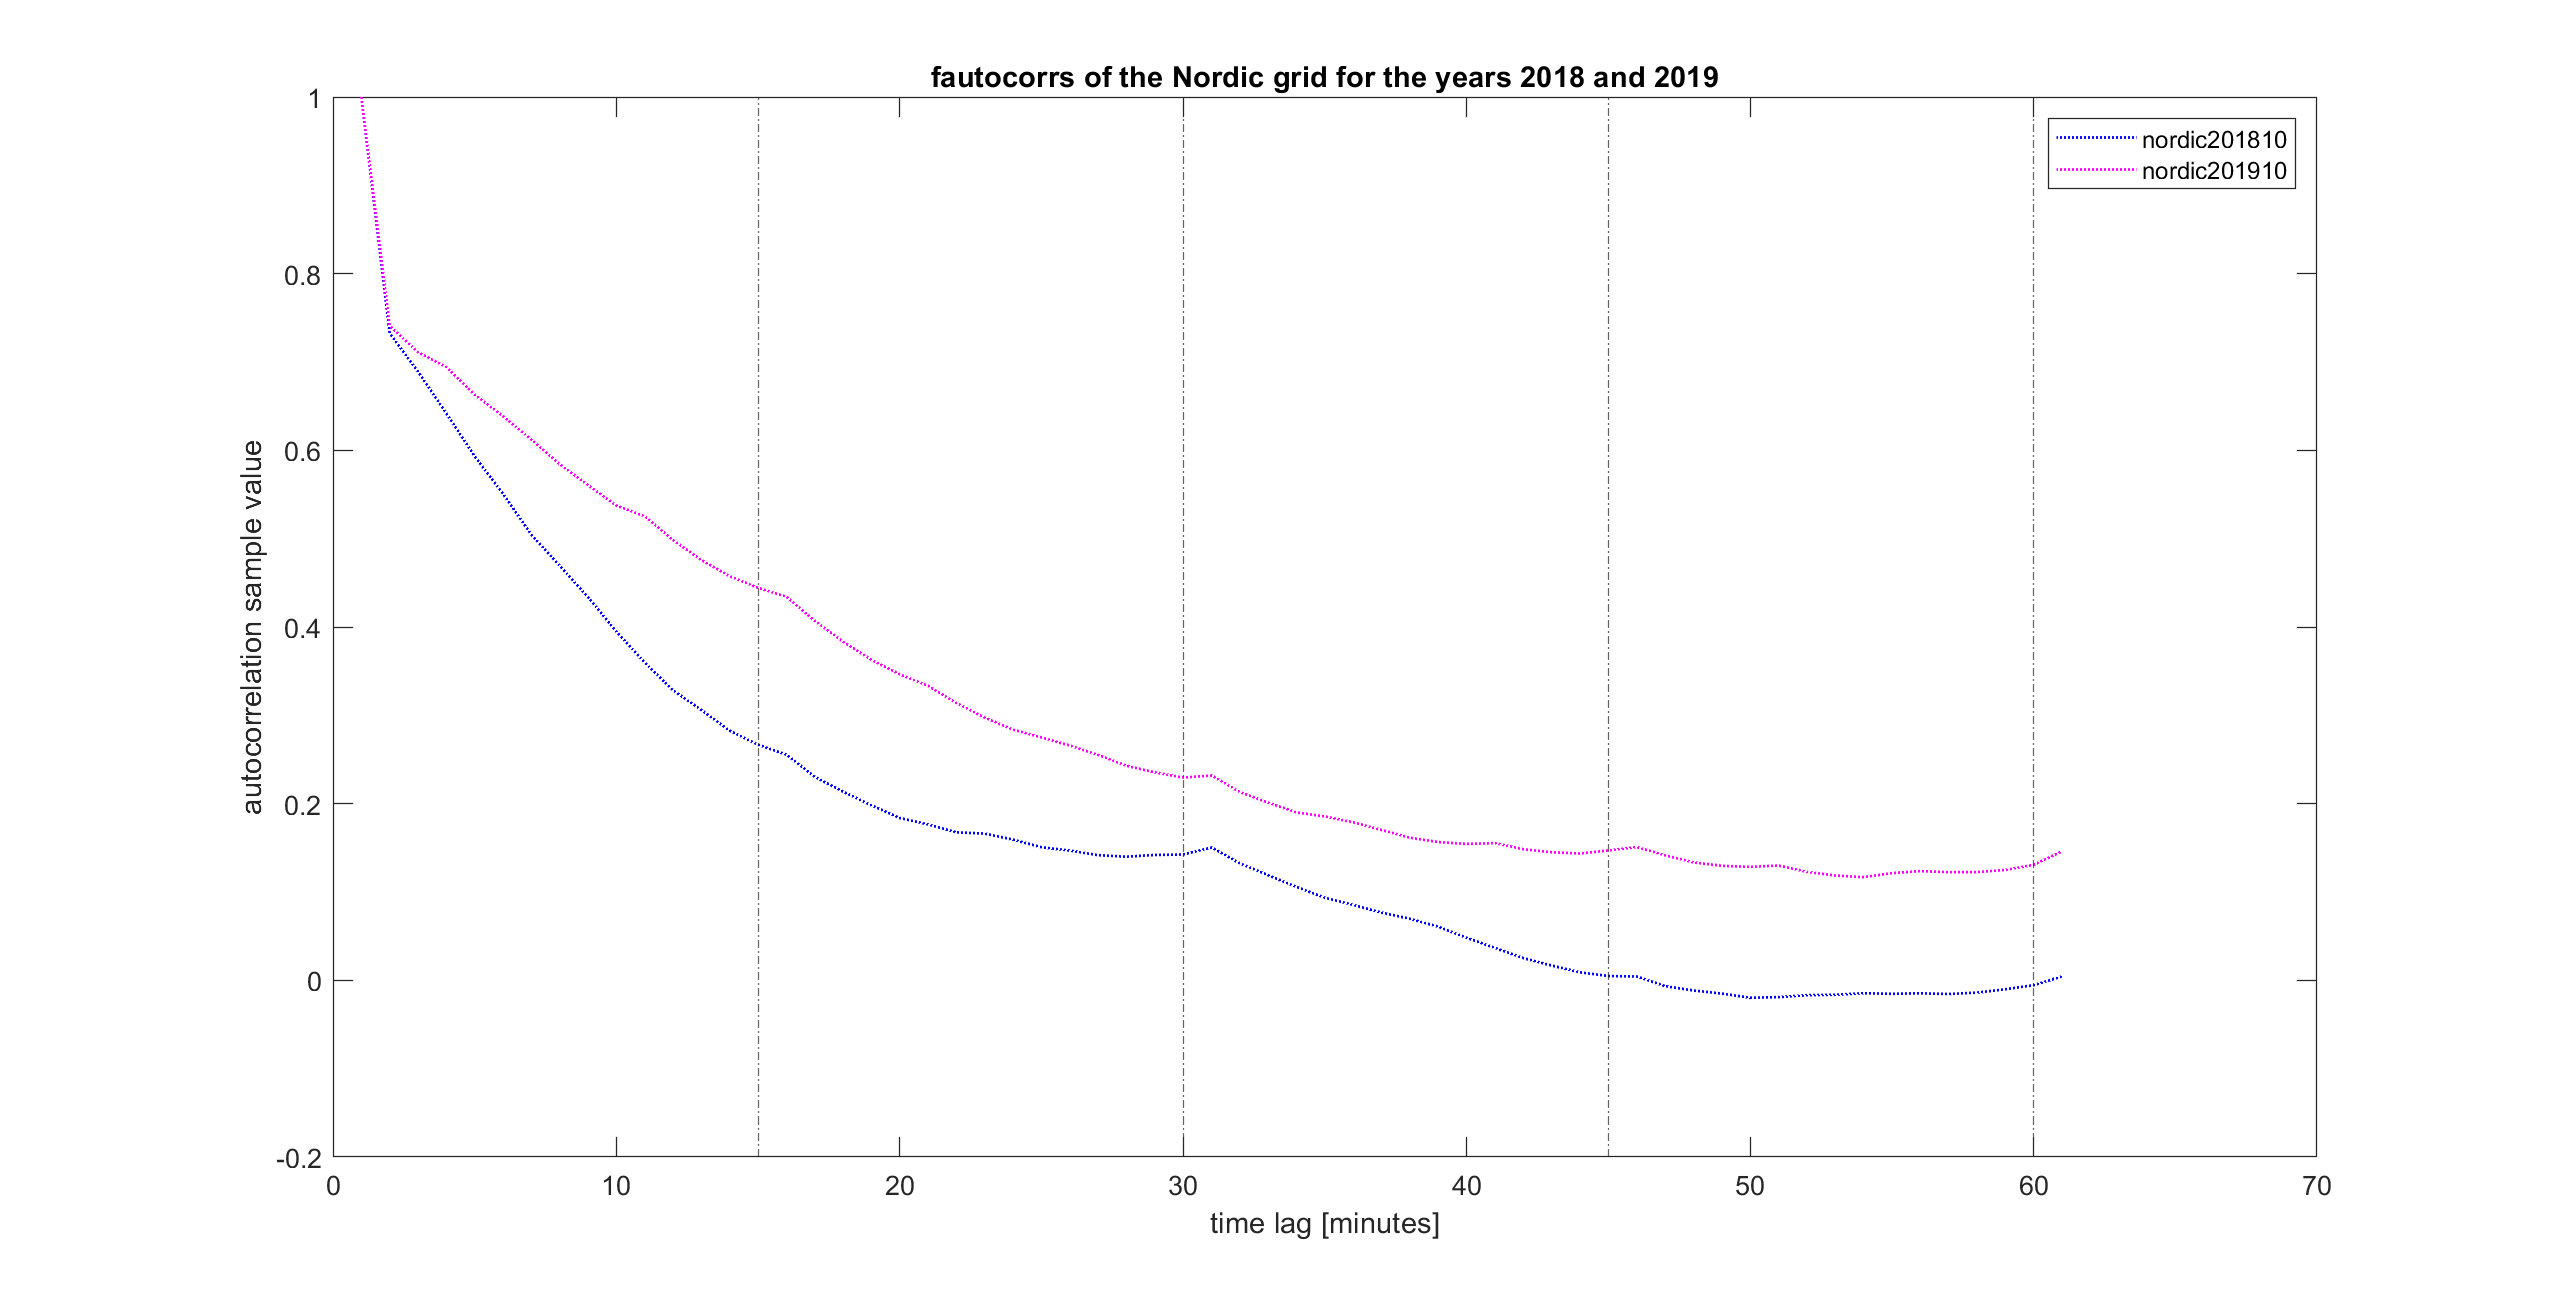
\includegraphics[scale=0.25]{../figures/autocorr/fautocorrs_nordic_201801_to_201912}
	\caption{Fixed Time Autocorrelation plots for the Nordic Grid for two consecutive years, 2018 and 2019. They present a fairly consistent picture of the grid's dynamics, with only a minor difference in the magnitude of the autocorrelation values.}
\end{figure}


\begin{figure}[!ht]
	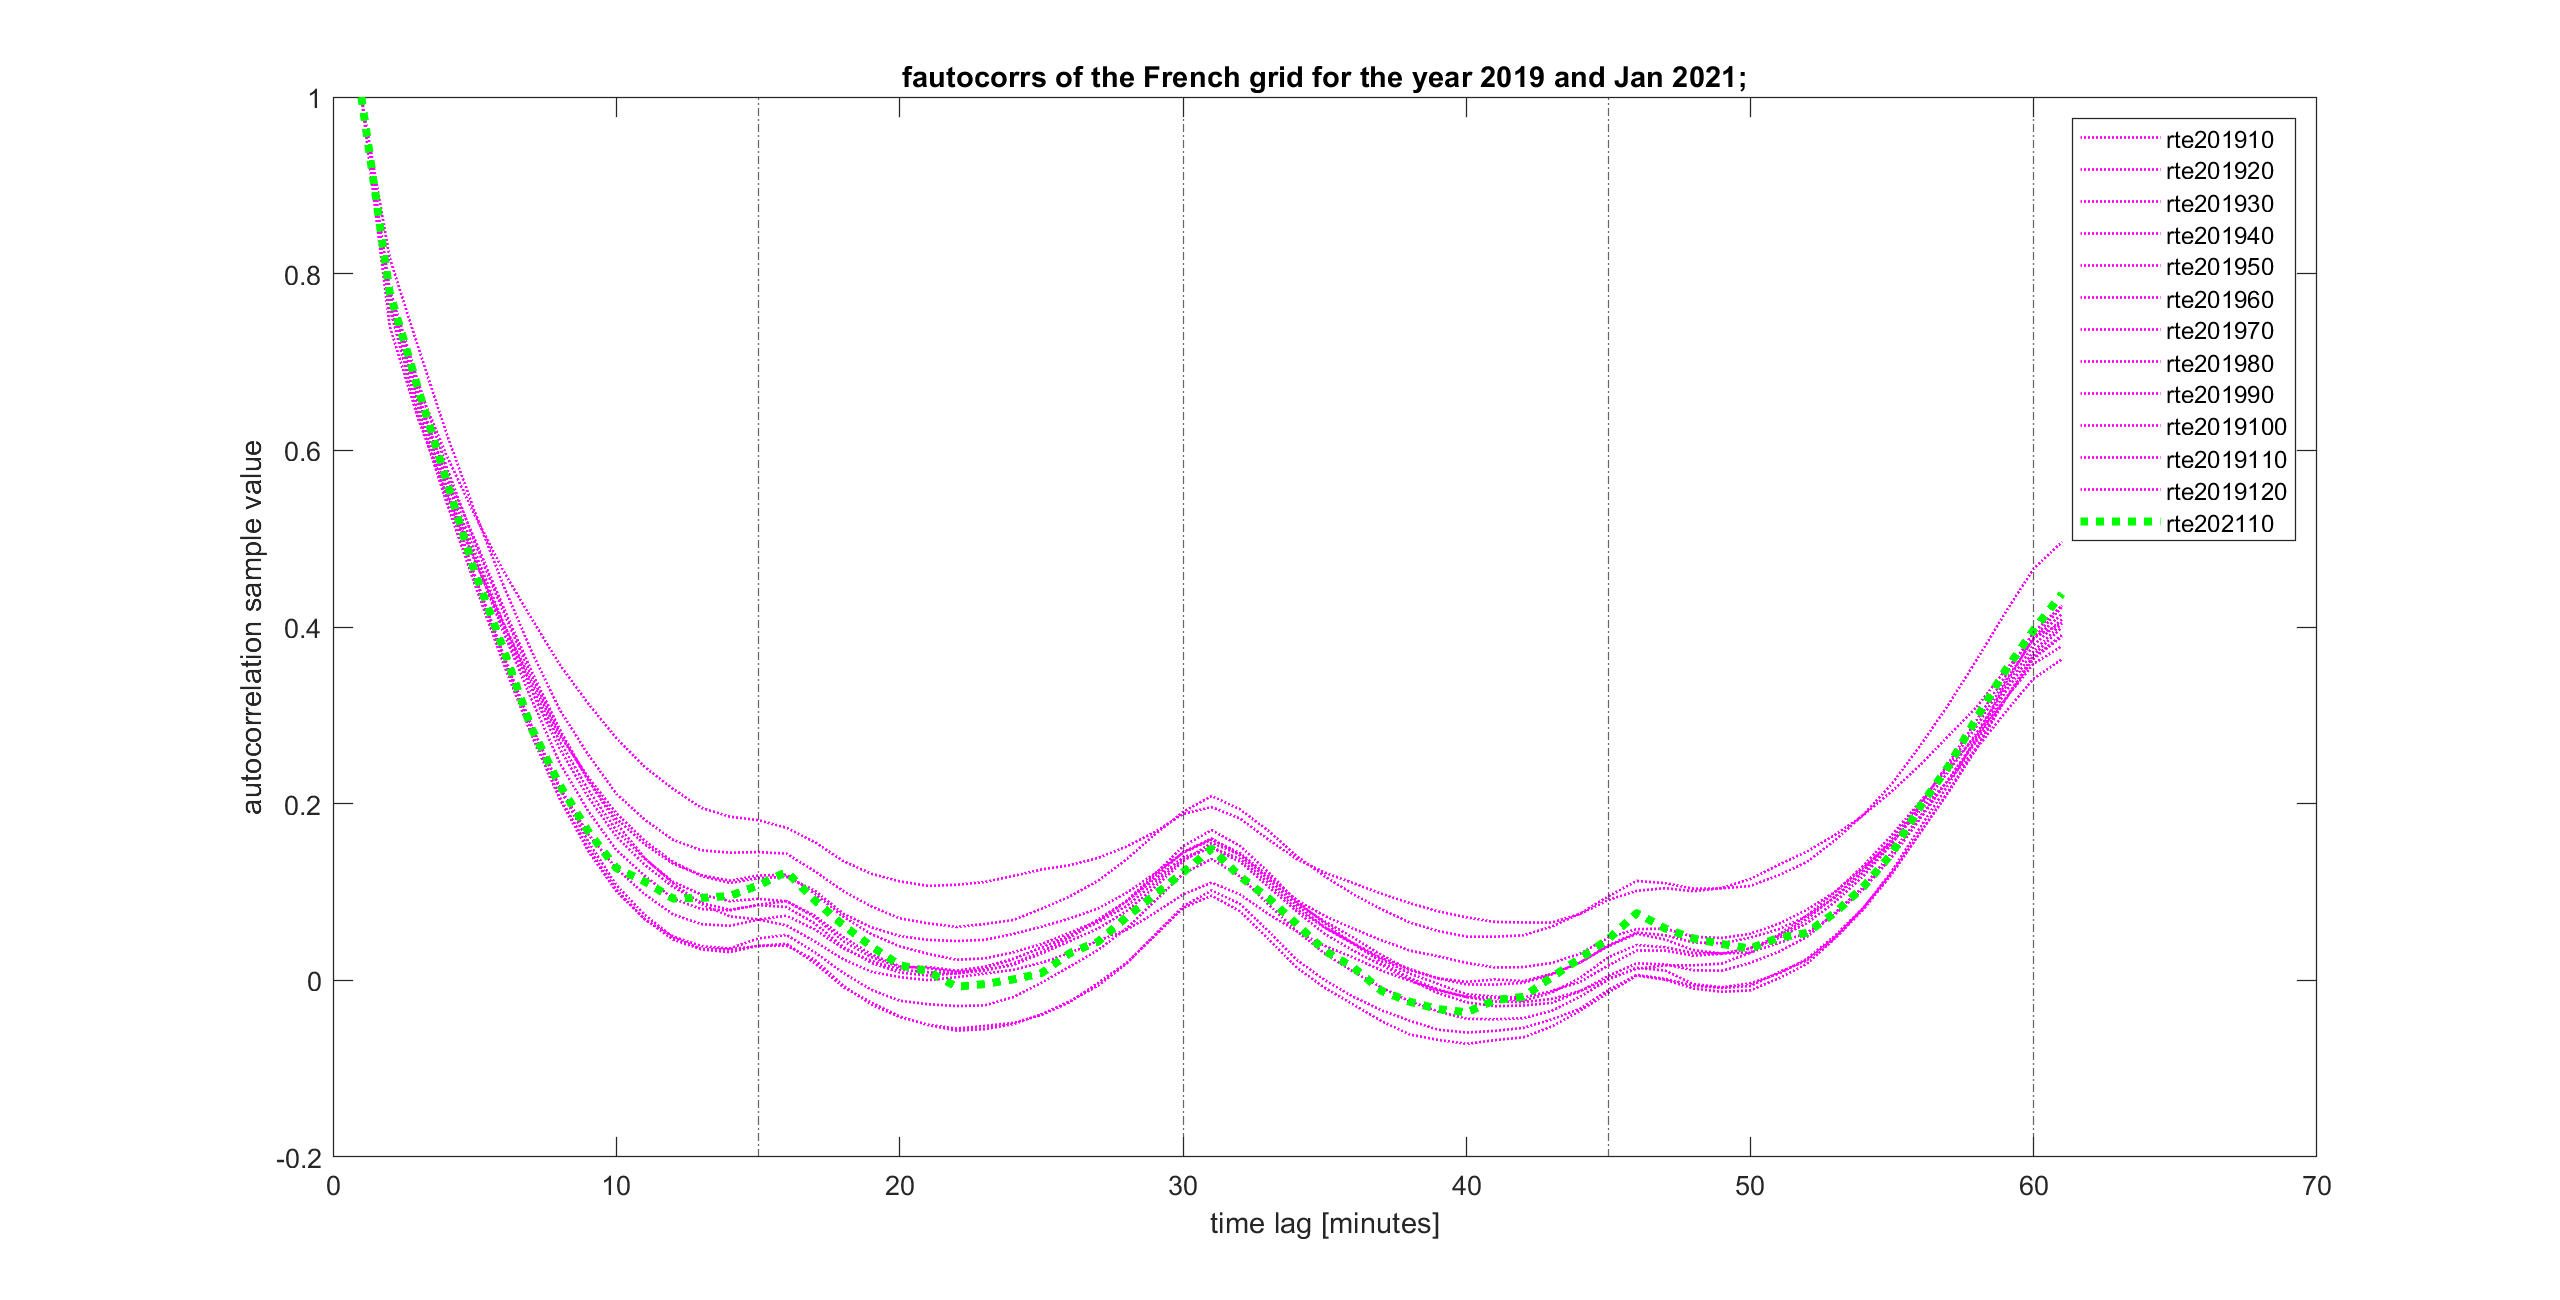
\includegraphics[scale=0.25]{../figures/autocorr/fautocorrs_rte_201901_to_201912_202101}
	\caption{Fixed Time Autocorrelation plots for the French Grid for twelve months of the year 2019 and January 2021. They present a fairly consistent picture of the grid's dynamics.}
\end{figure}

\begin{figure}[!ht]
	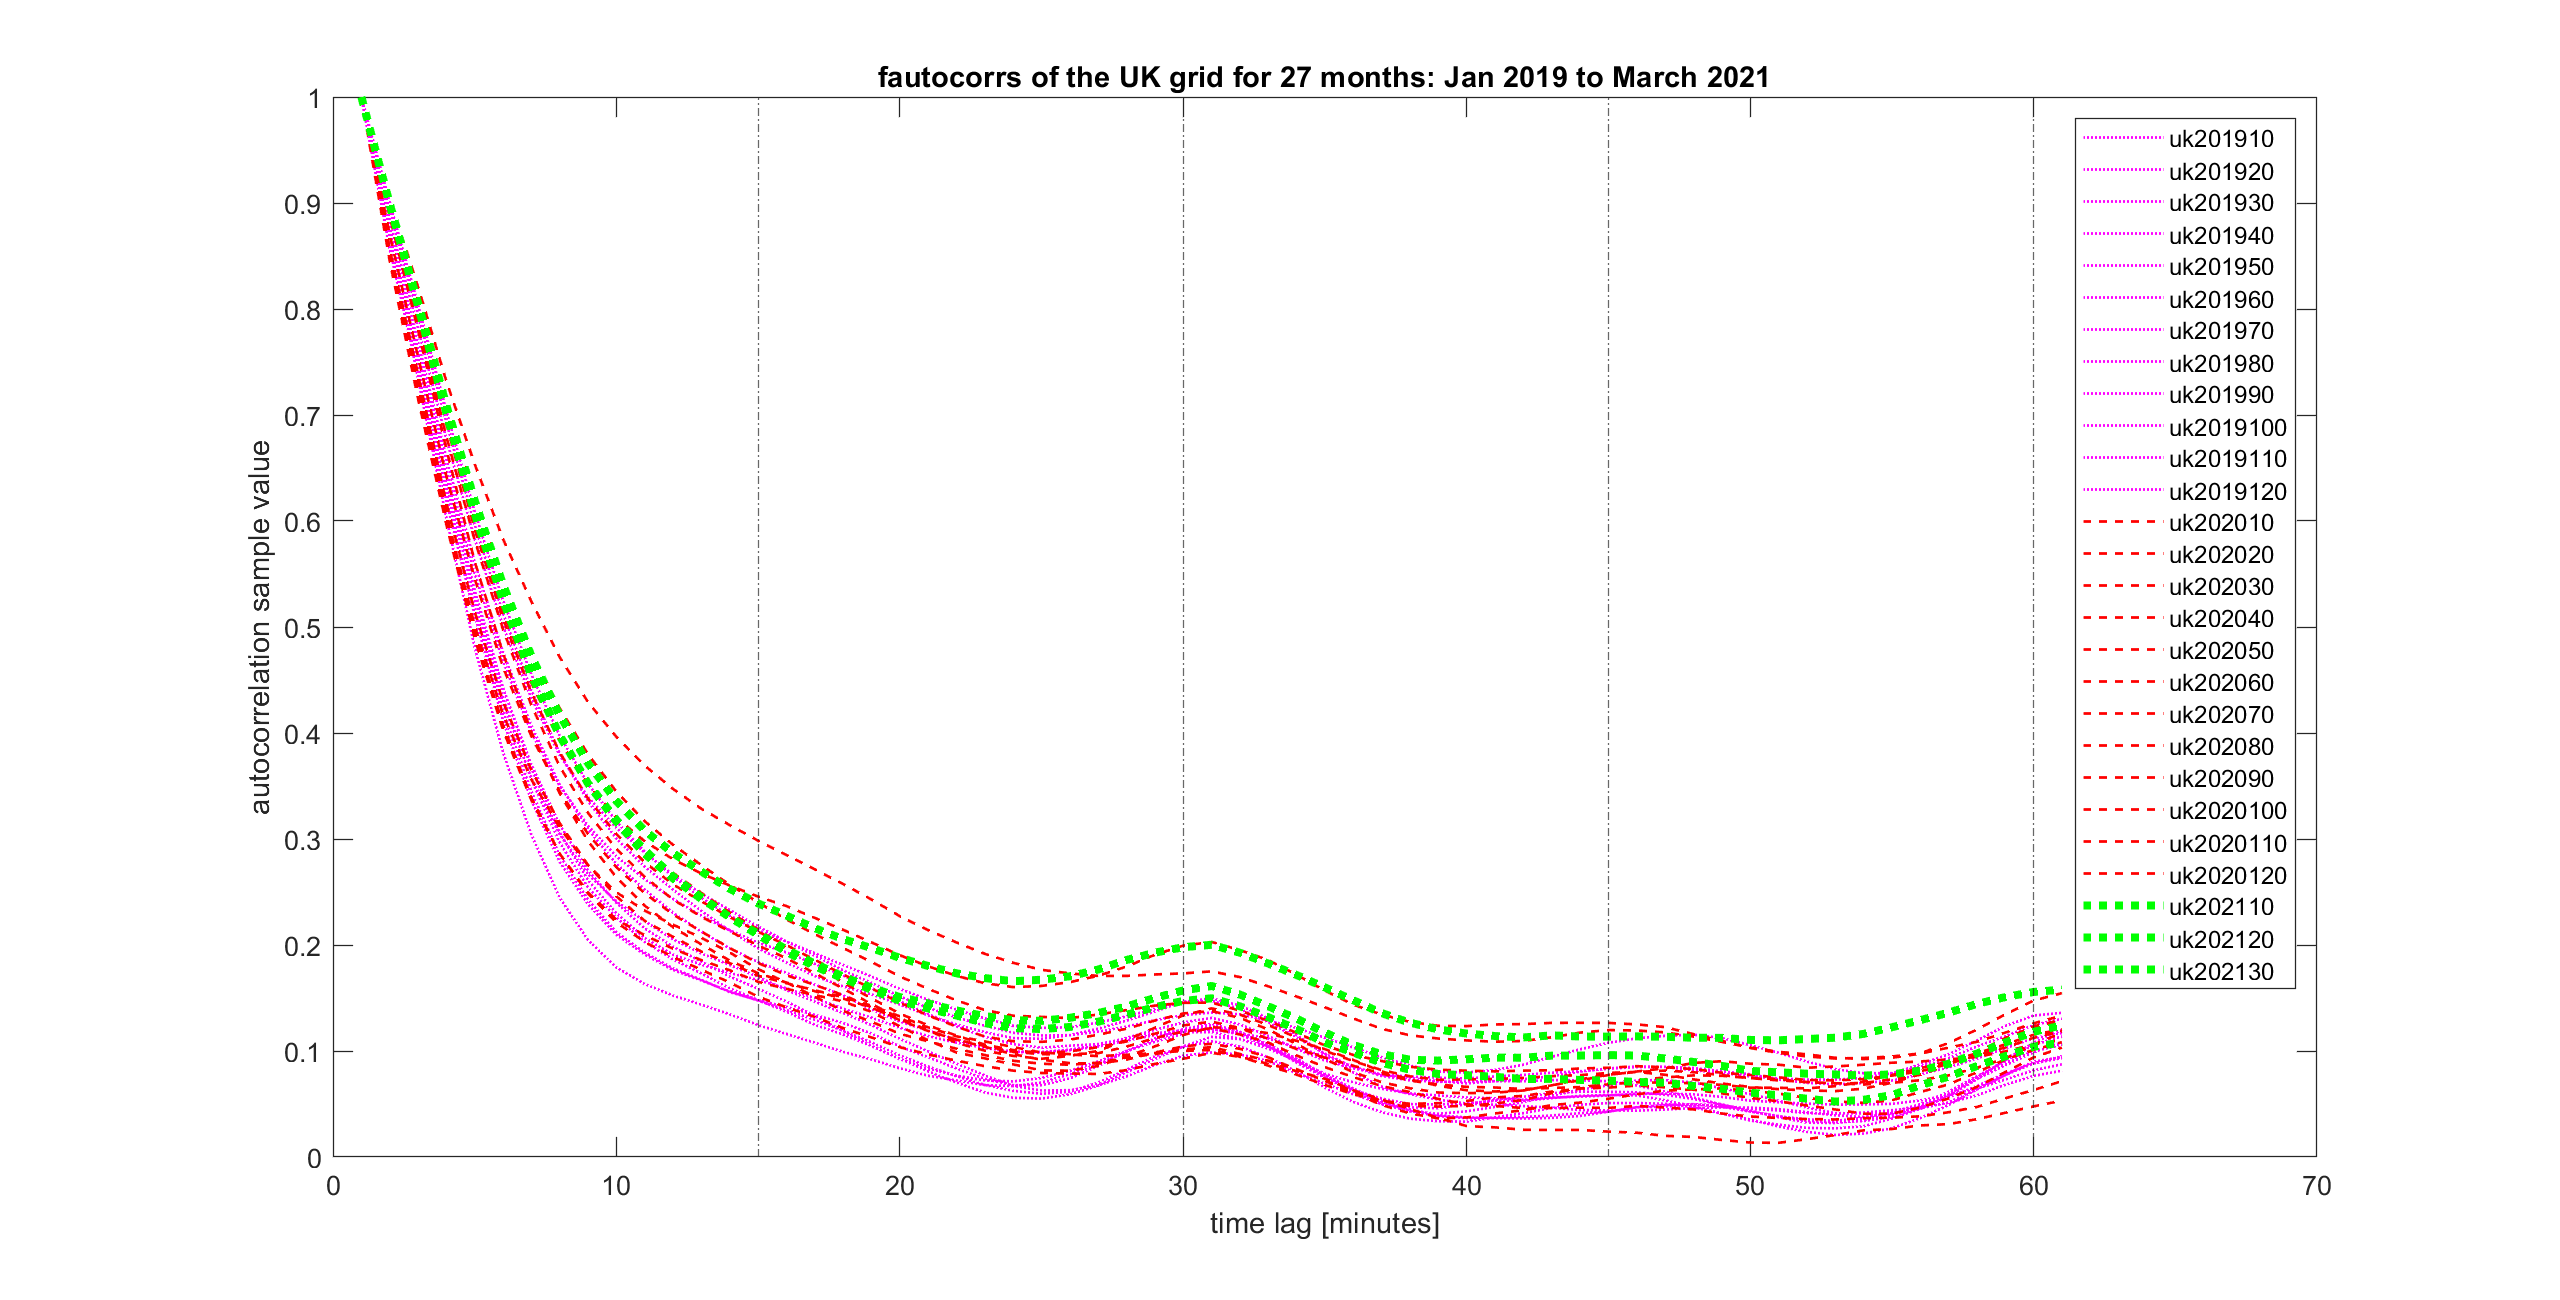
\includegraphics[scale=0.25]{../figures/autocorr/fautocorrs_uk_201901_to_202103_2}
	\caption{Fixed Time Autocorrelation plots for the Great Britain Grid for twenty seven continuous months, from January 2019 to March 2021. They present a fairly consistent picture of the grid's dynamics.}
\end{figure}

\begin{figure}[!ht]
	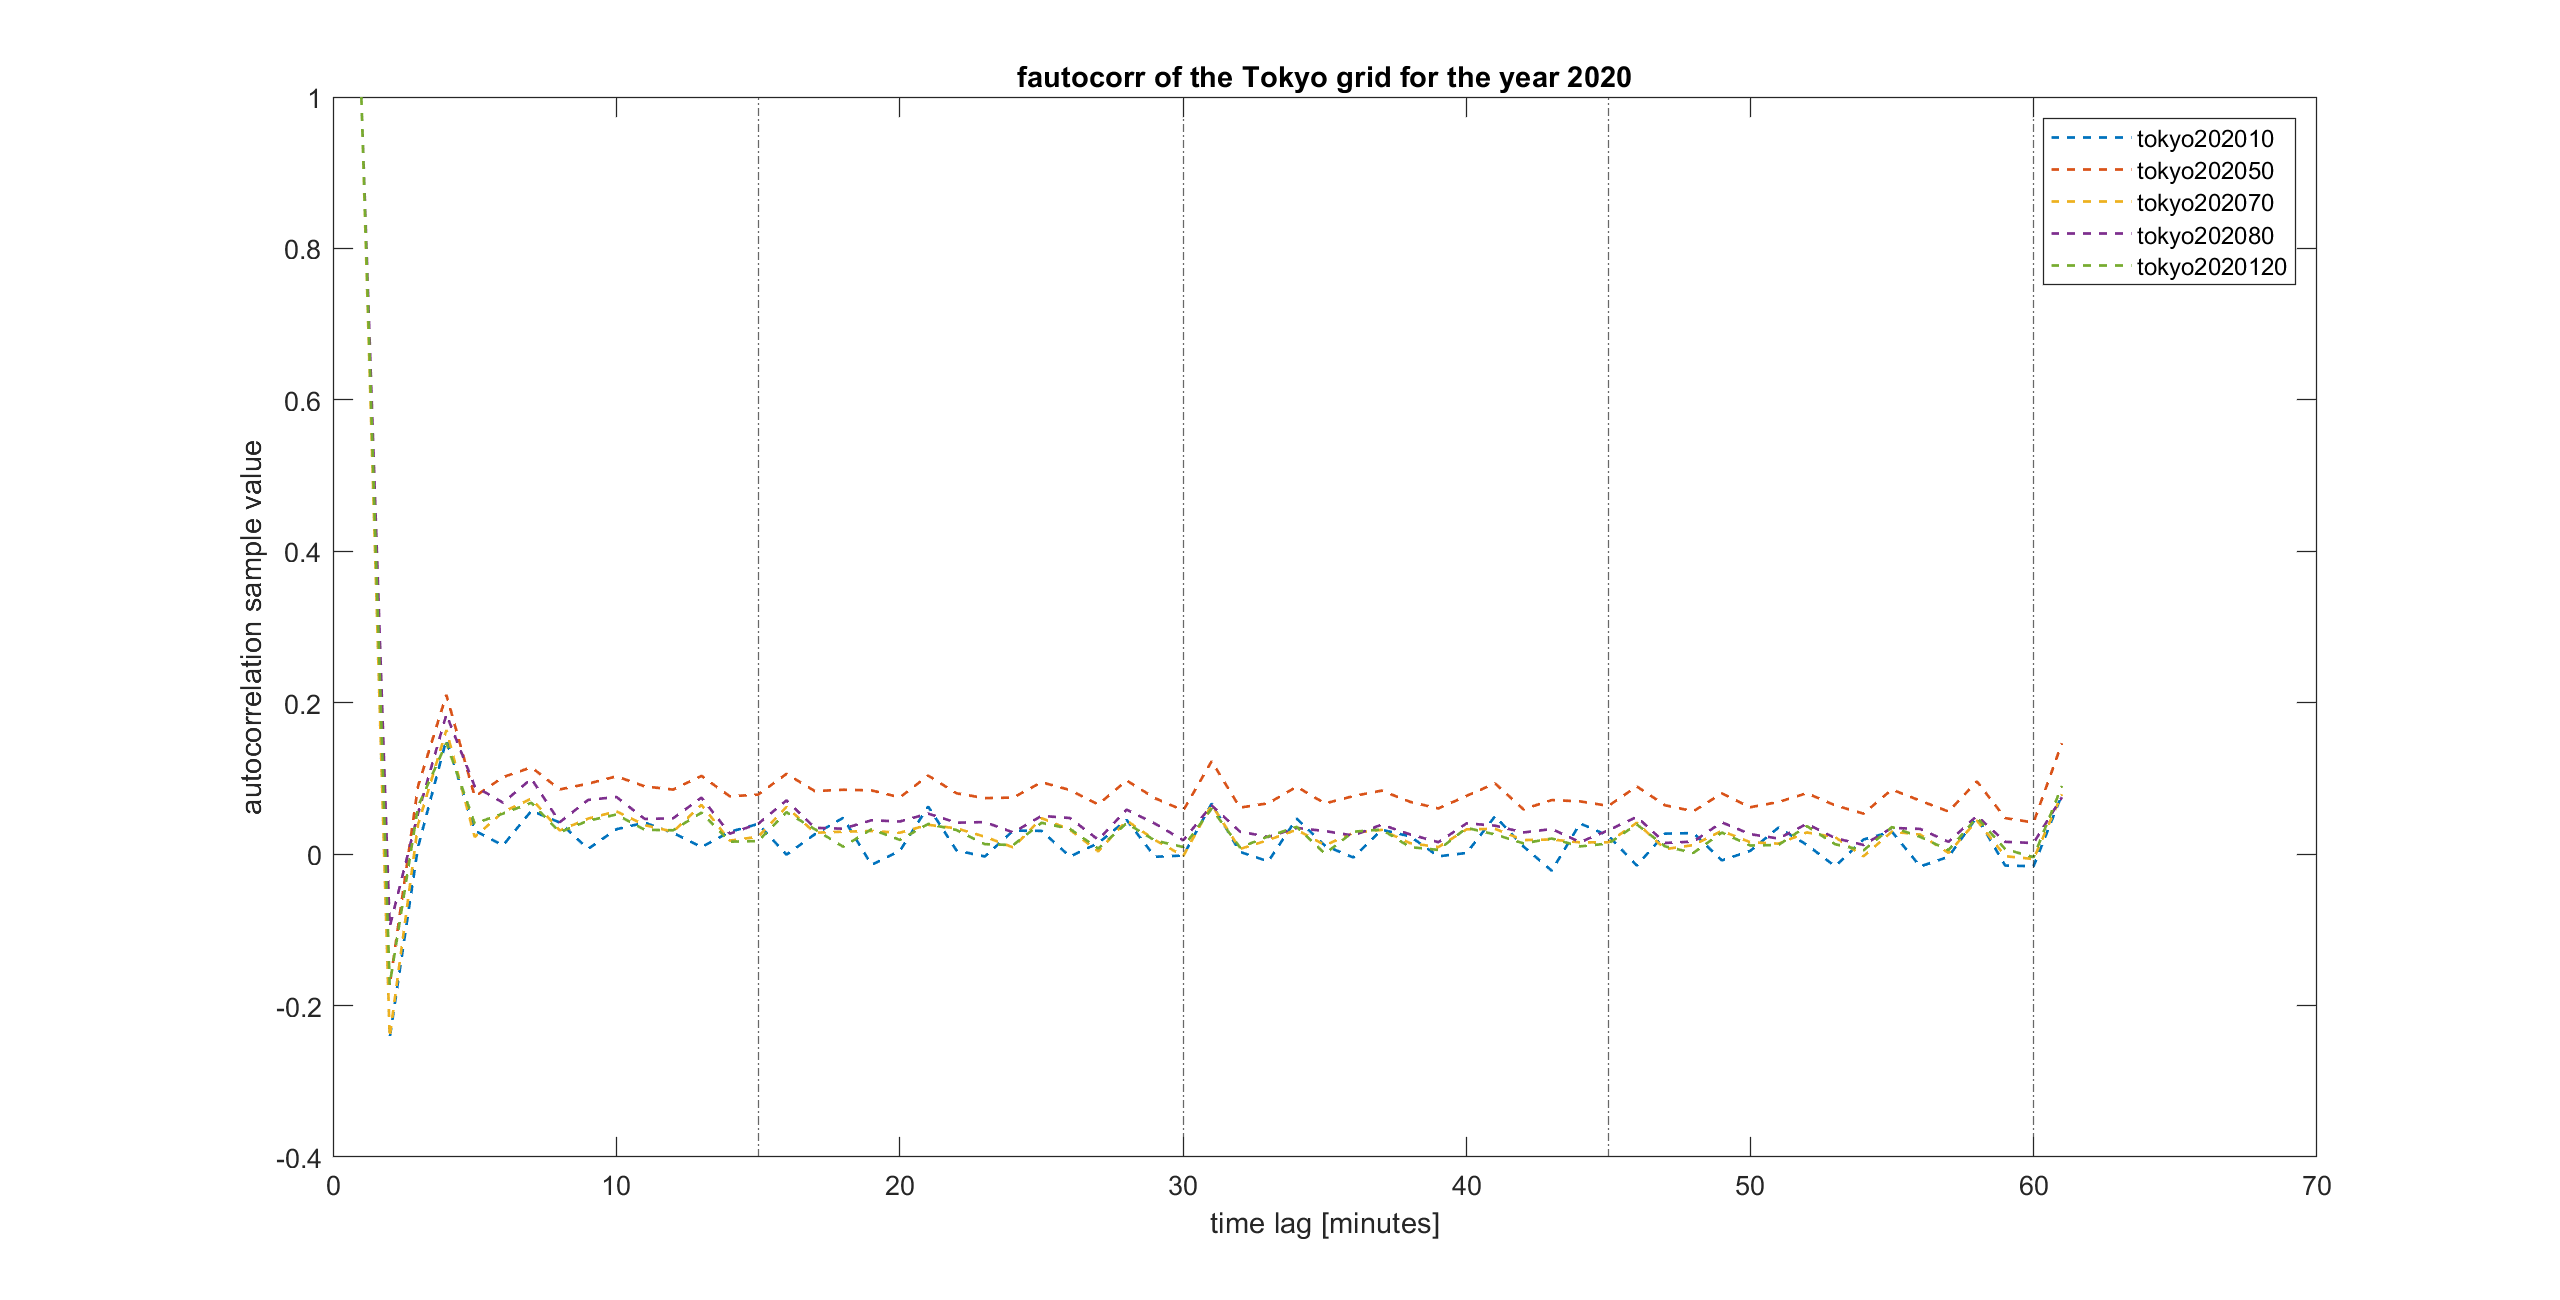
\includegraphics[scale=0.25]{../figures/autocorr/fautocorrs_tokyo_202001_to_202012}
	\caption{Fixed Time Autocorrelation plots for the Tokyo Grid for five non-continuous months of the year 2020: January, May, July, August and December. They present a fairly consistent picture of the grid's dynamics.}
\end{figure}

Data for six non-continuous days (07 April 2019, 03 July 2019, 08 August 2019, 14 December 2019, 01 February 2020 and 05 April 2020) for the Indian grid (NRLDC) was also compared in a similar fashion. Some of the days have also been marked with attributes to indicate notable demand-generation characteristics associated with the day, including: Day with minimum renewable generation, Day with maximum renewable generation contribution (07 April 2019), Day with minimum solar power contribution (08 August 2019), Day with lowest power demand (14 December 2019) and Day with lowest renewable generation contribution (01 February 2020). The plots were inconsistent and therefore a day's worth of data could be considered insufficient to average-out all the dynamic differences in a grid's statistical signature.

\begin{figure}[!ht]
	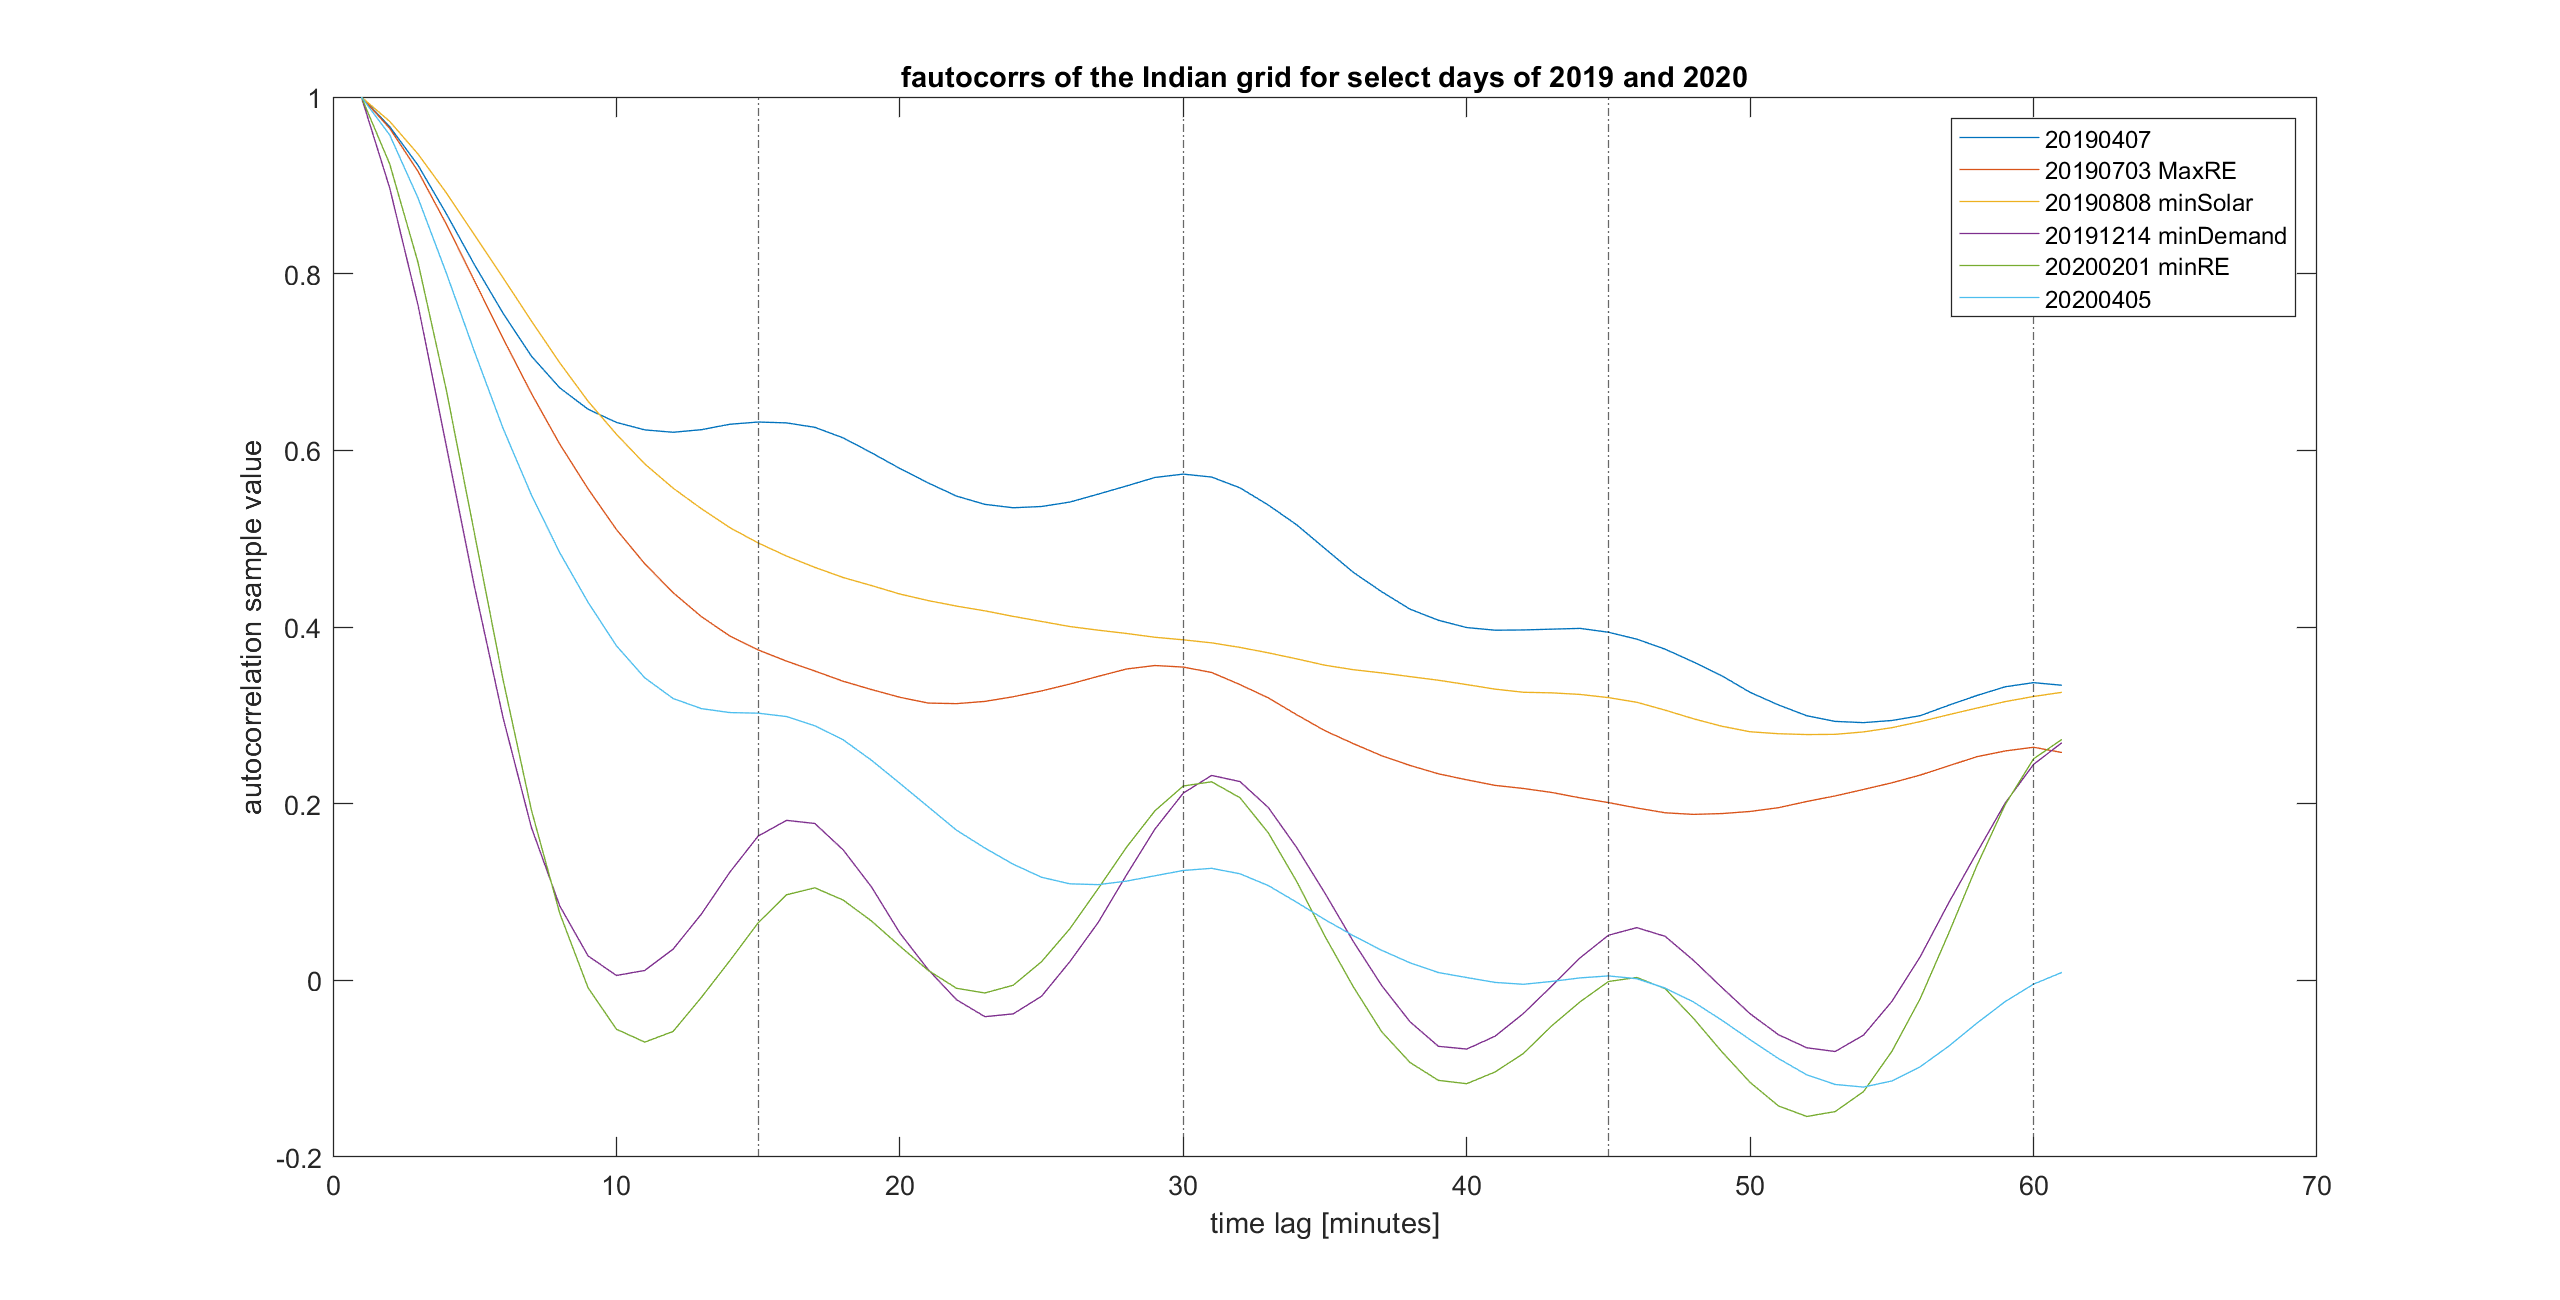
\includegraphics[scale=0.25]{../figures/autocorr/fautocorrs_nrldc_201904_to_202004}
	\caption{Fixed Time Autocorrelation Plots for Six non-continuous days of the Indian Grid: 07 April 2019, 03 July 2019, 08 August 2019, 14 December 2019, 01 February 2020 and 05 April 2020. Some of the days have also been marked with attributes with notable demand-generation characteristics associated with the day.}
\end{figure}

\begin{figure}[htp]
	\centering
	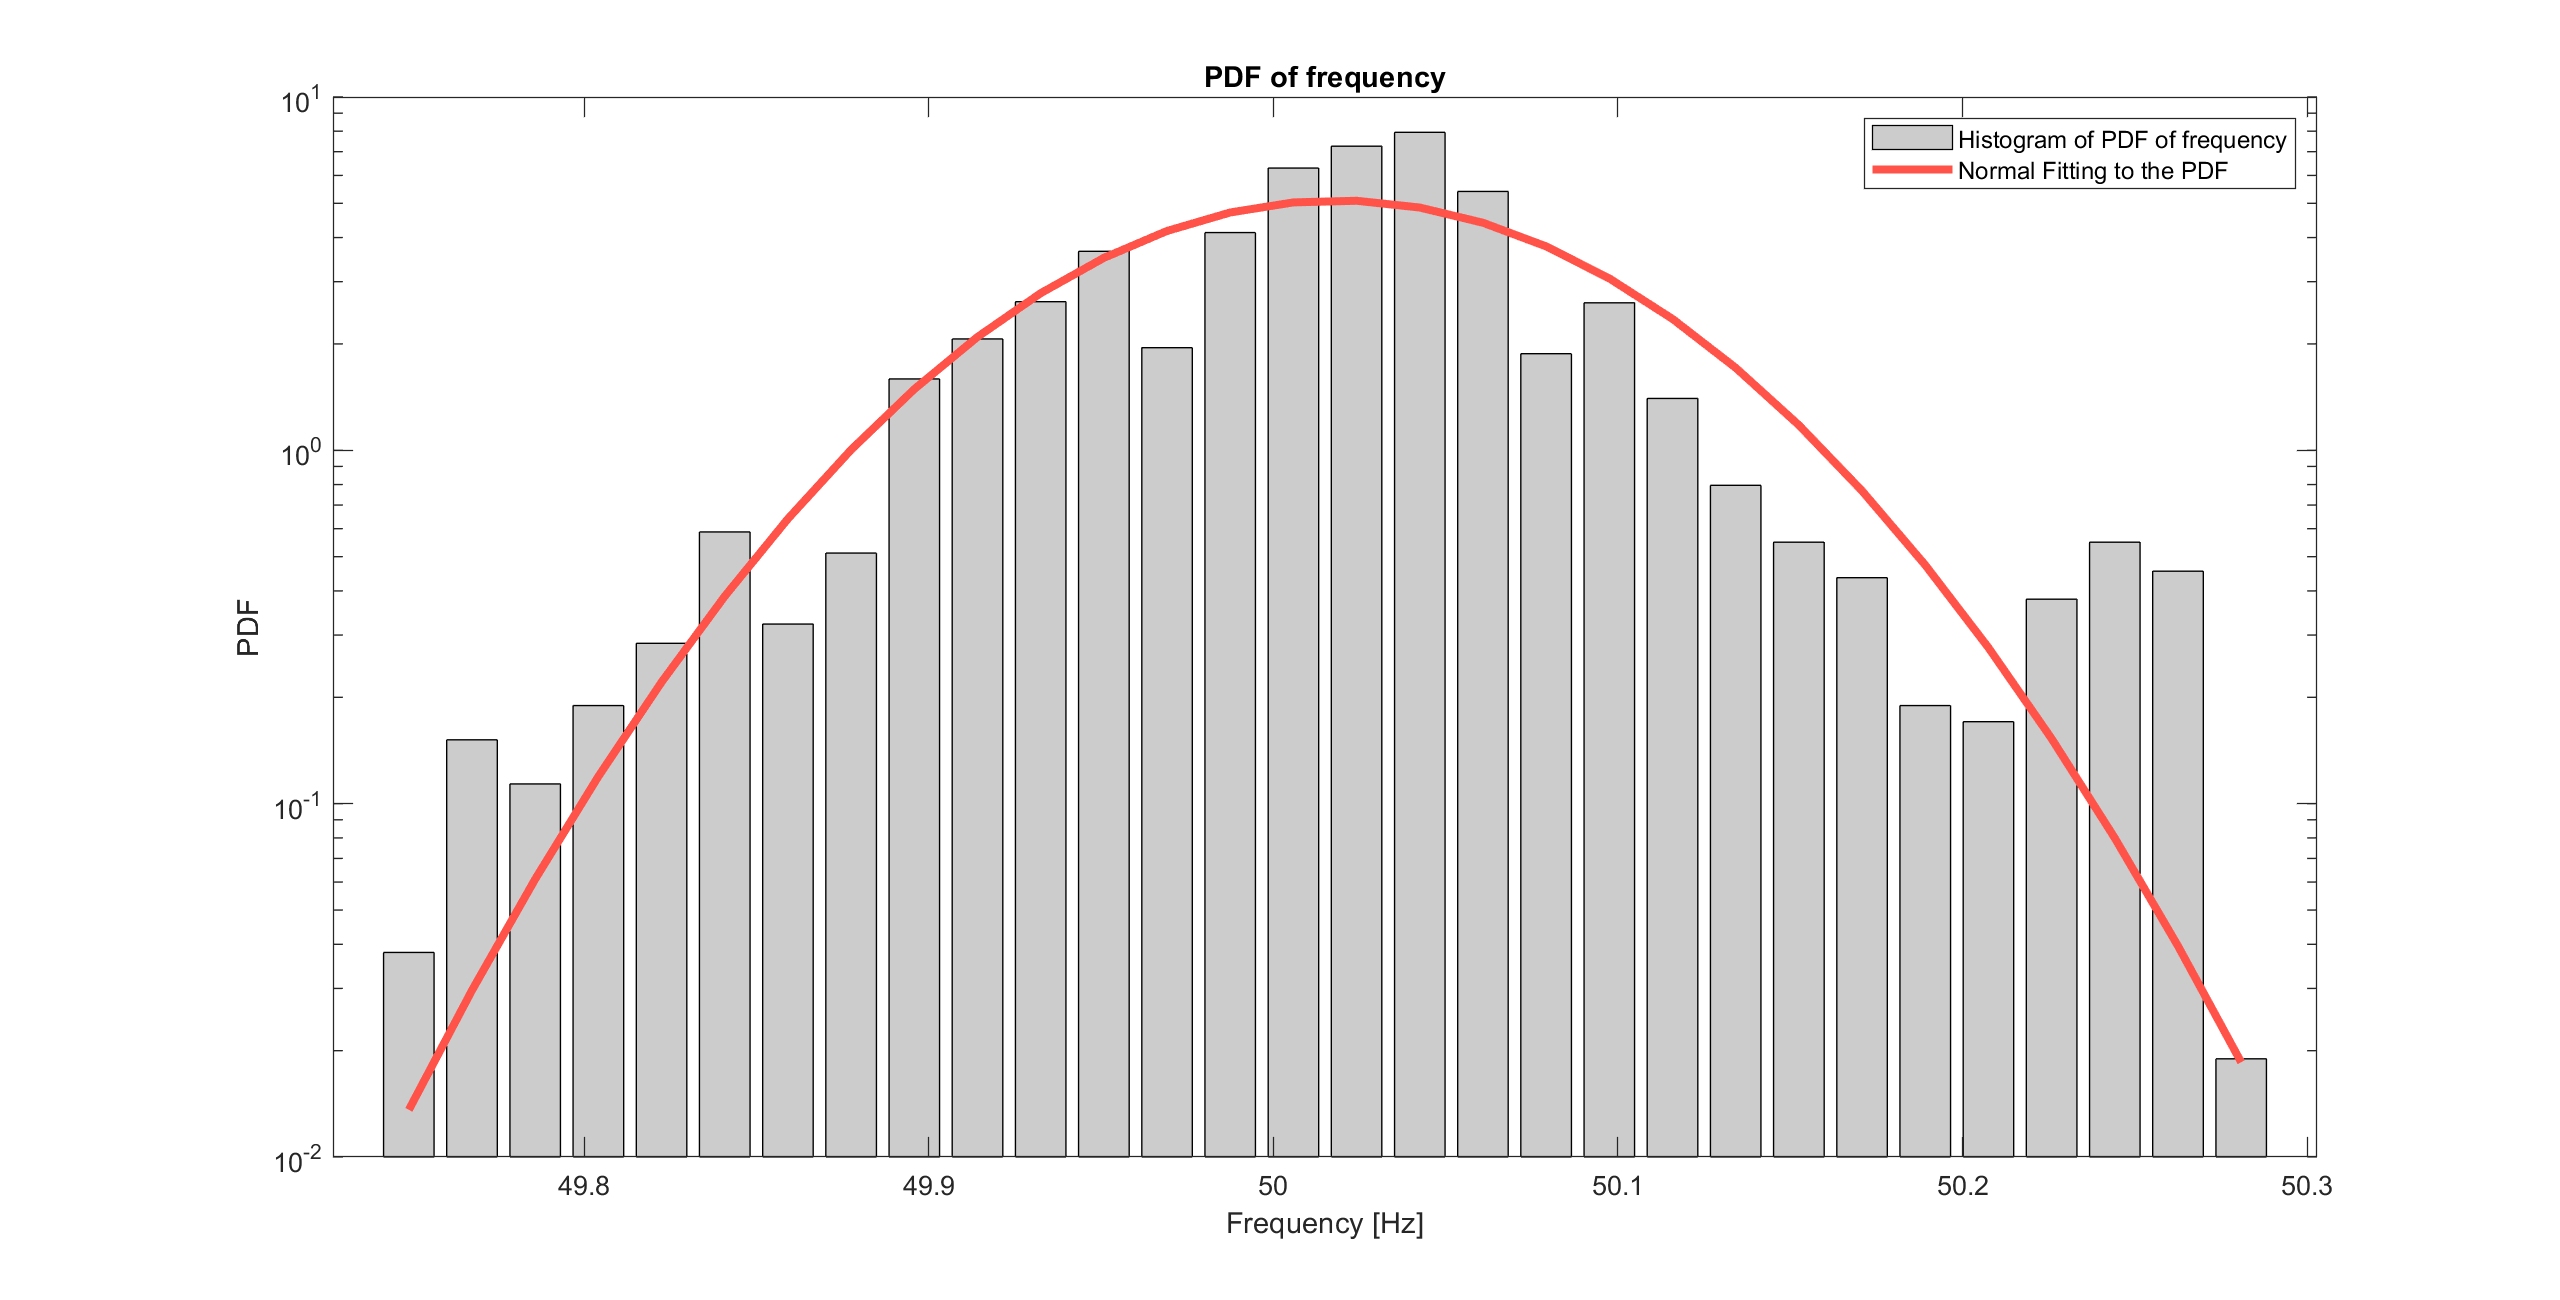
\includegraphics[width=.45\textwidth]{../figures/pdf/nrldc/pdf_frequency_nrldc_01}\quad
	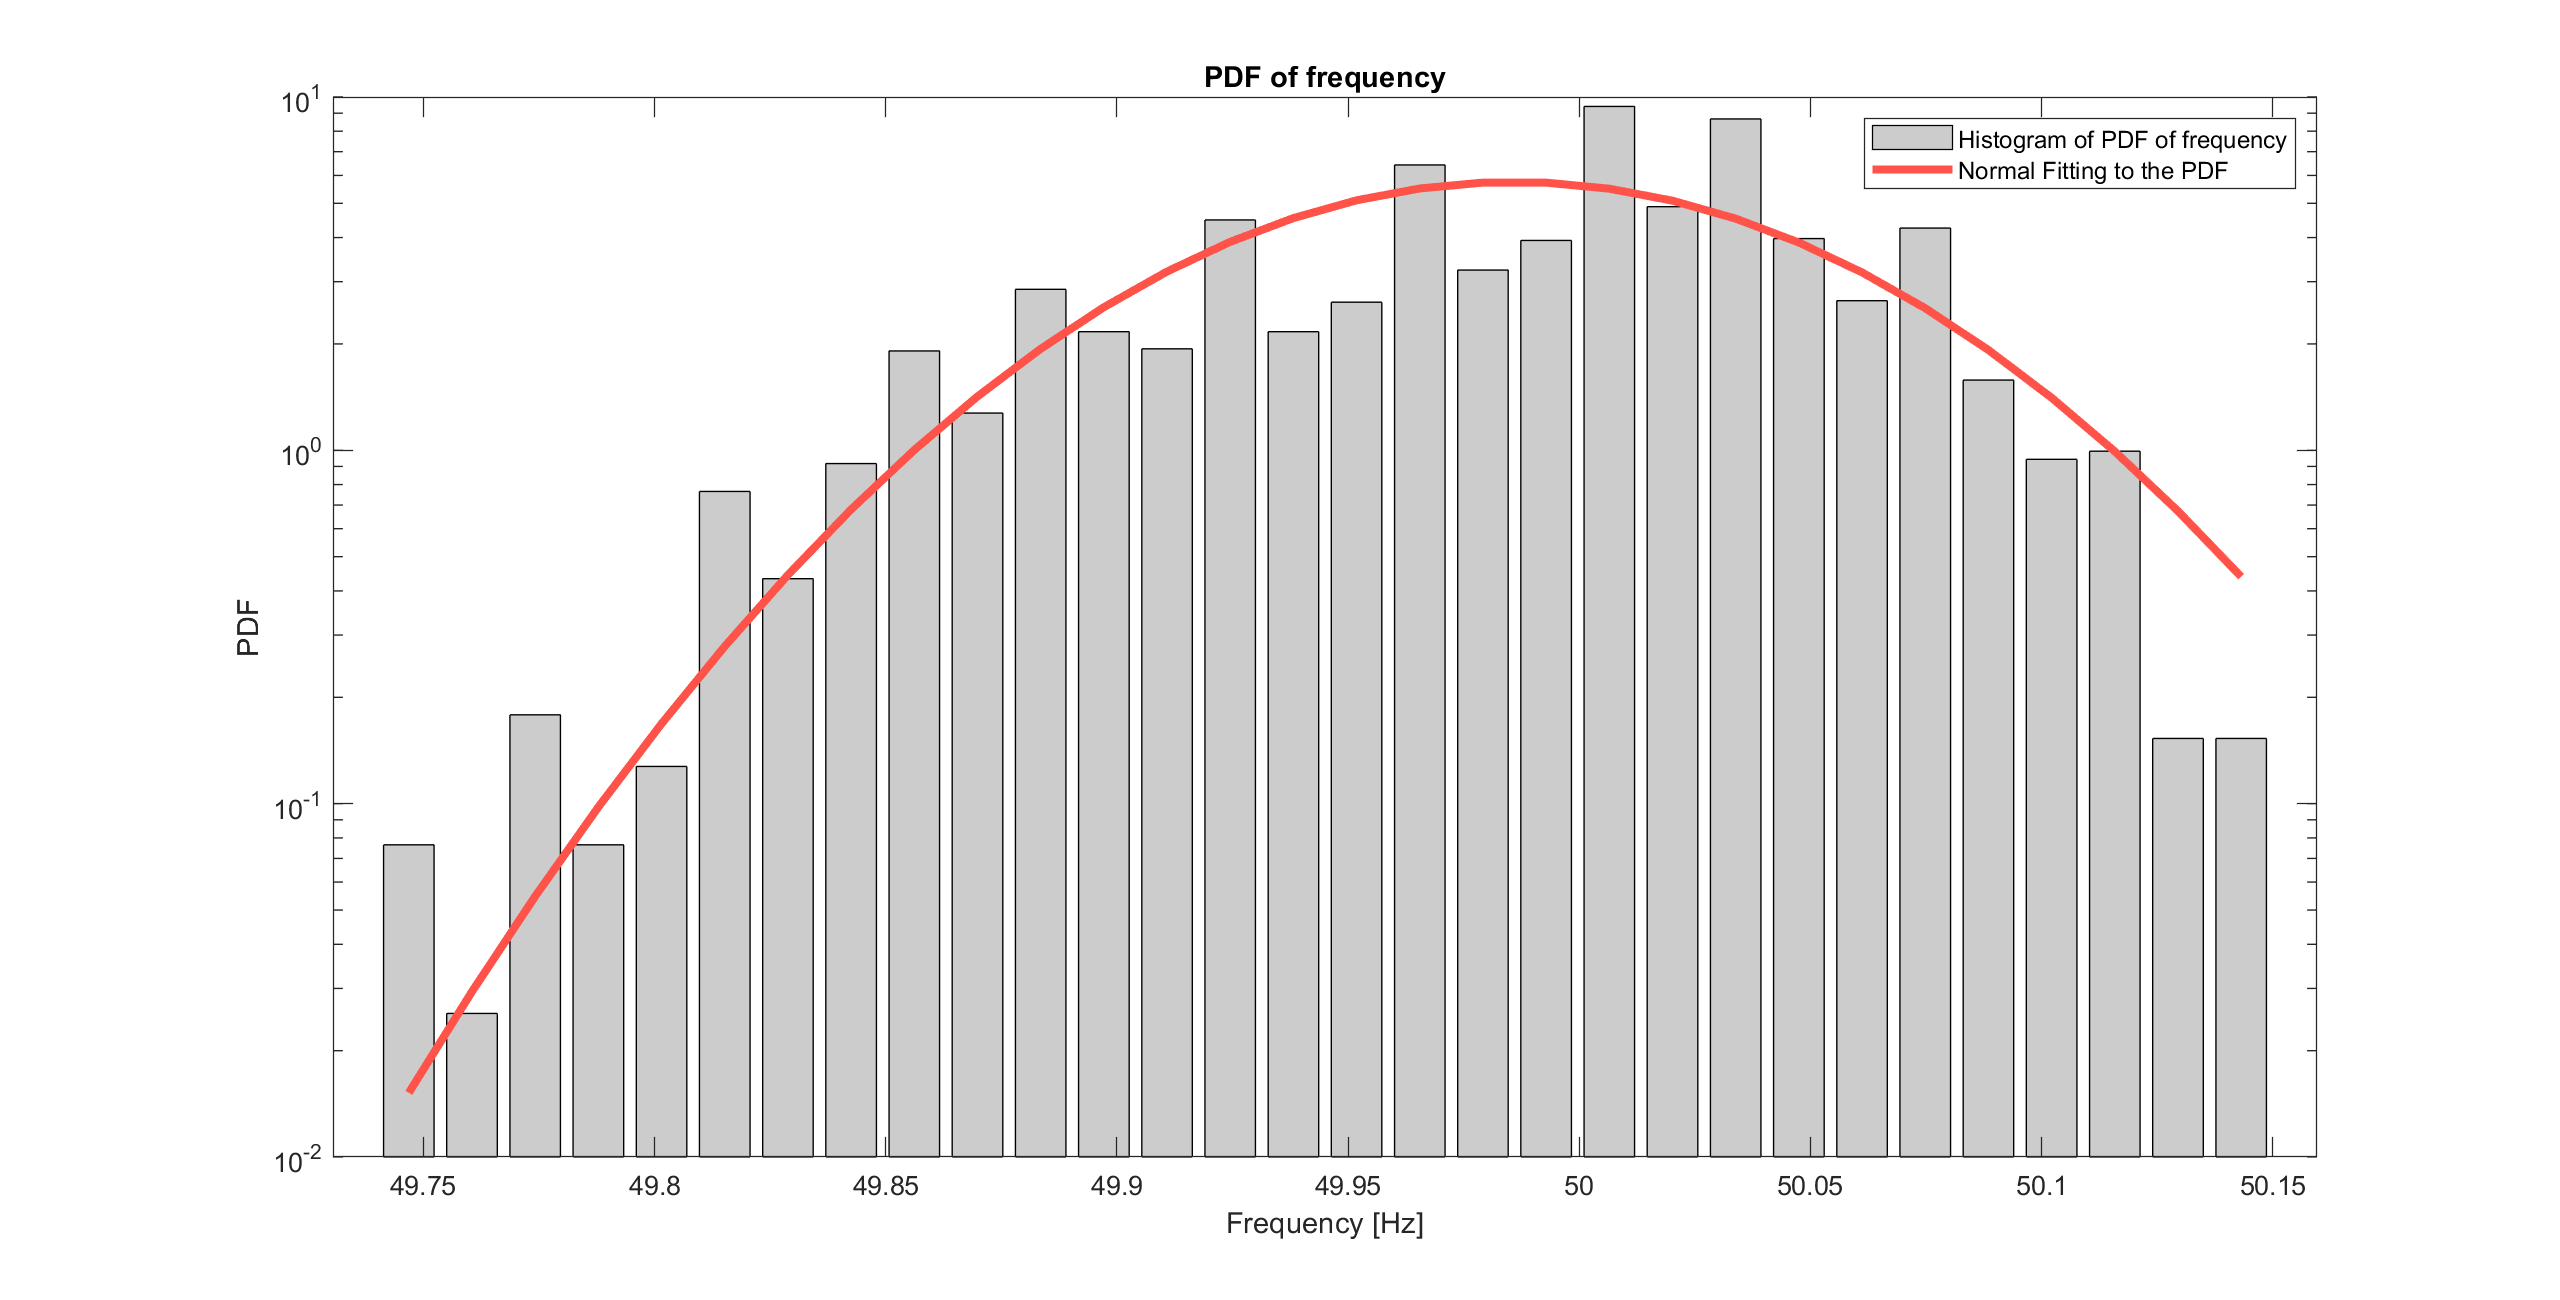
\includegraphics[width=.45\textwidth]{../figures/pdf/nrldc/pdf_frequency_nrldc_02}
	
	\medskip
	
	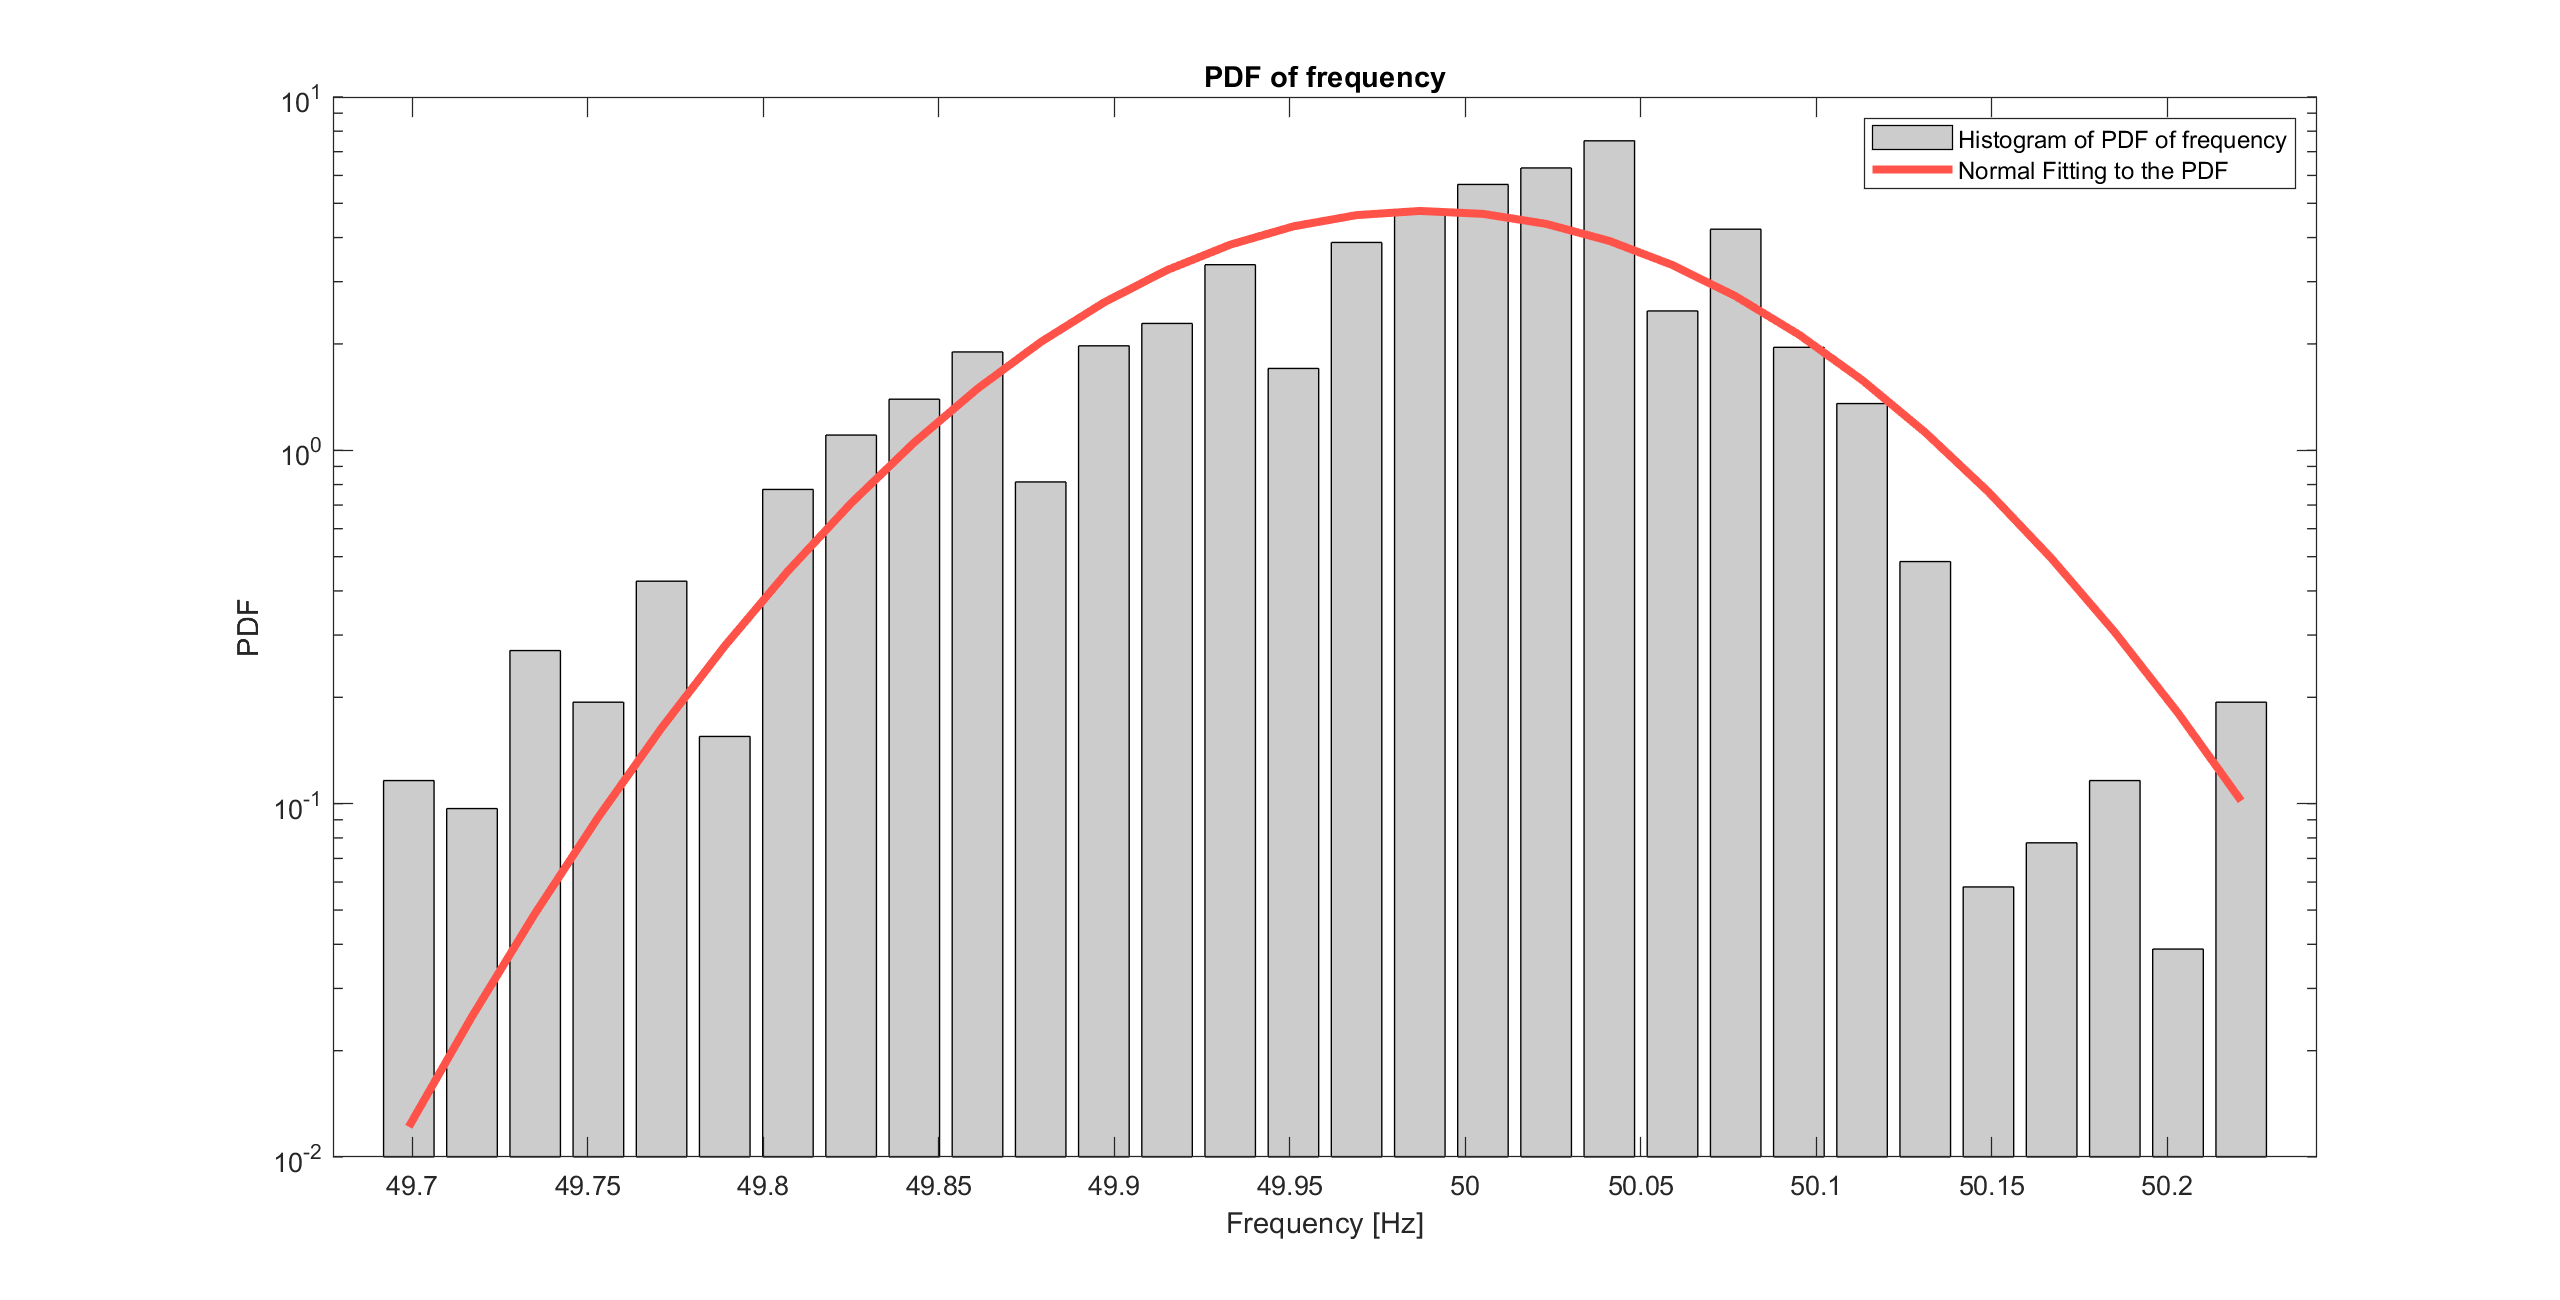
\includegraphics[width=.45\textwidth]{../figures/pdf/nrldc/pdf_frequency_nrldc_03}\quad
	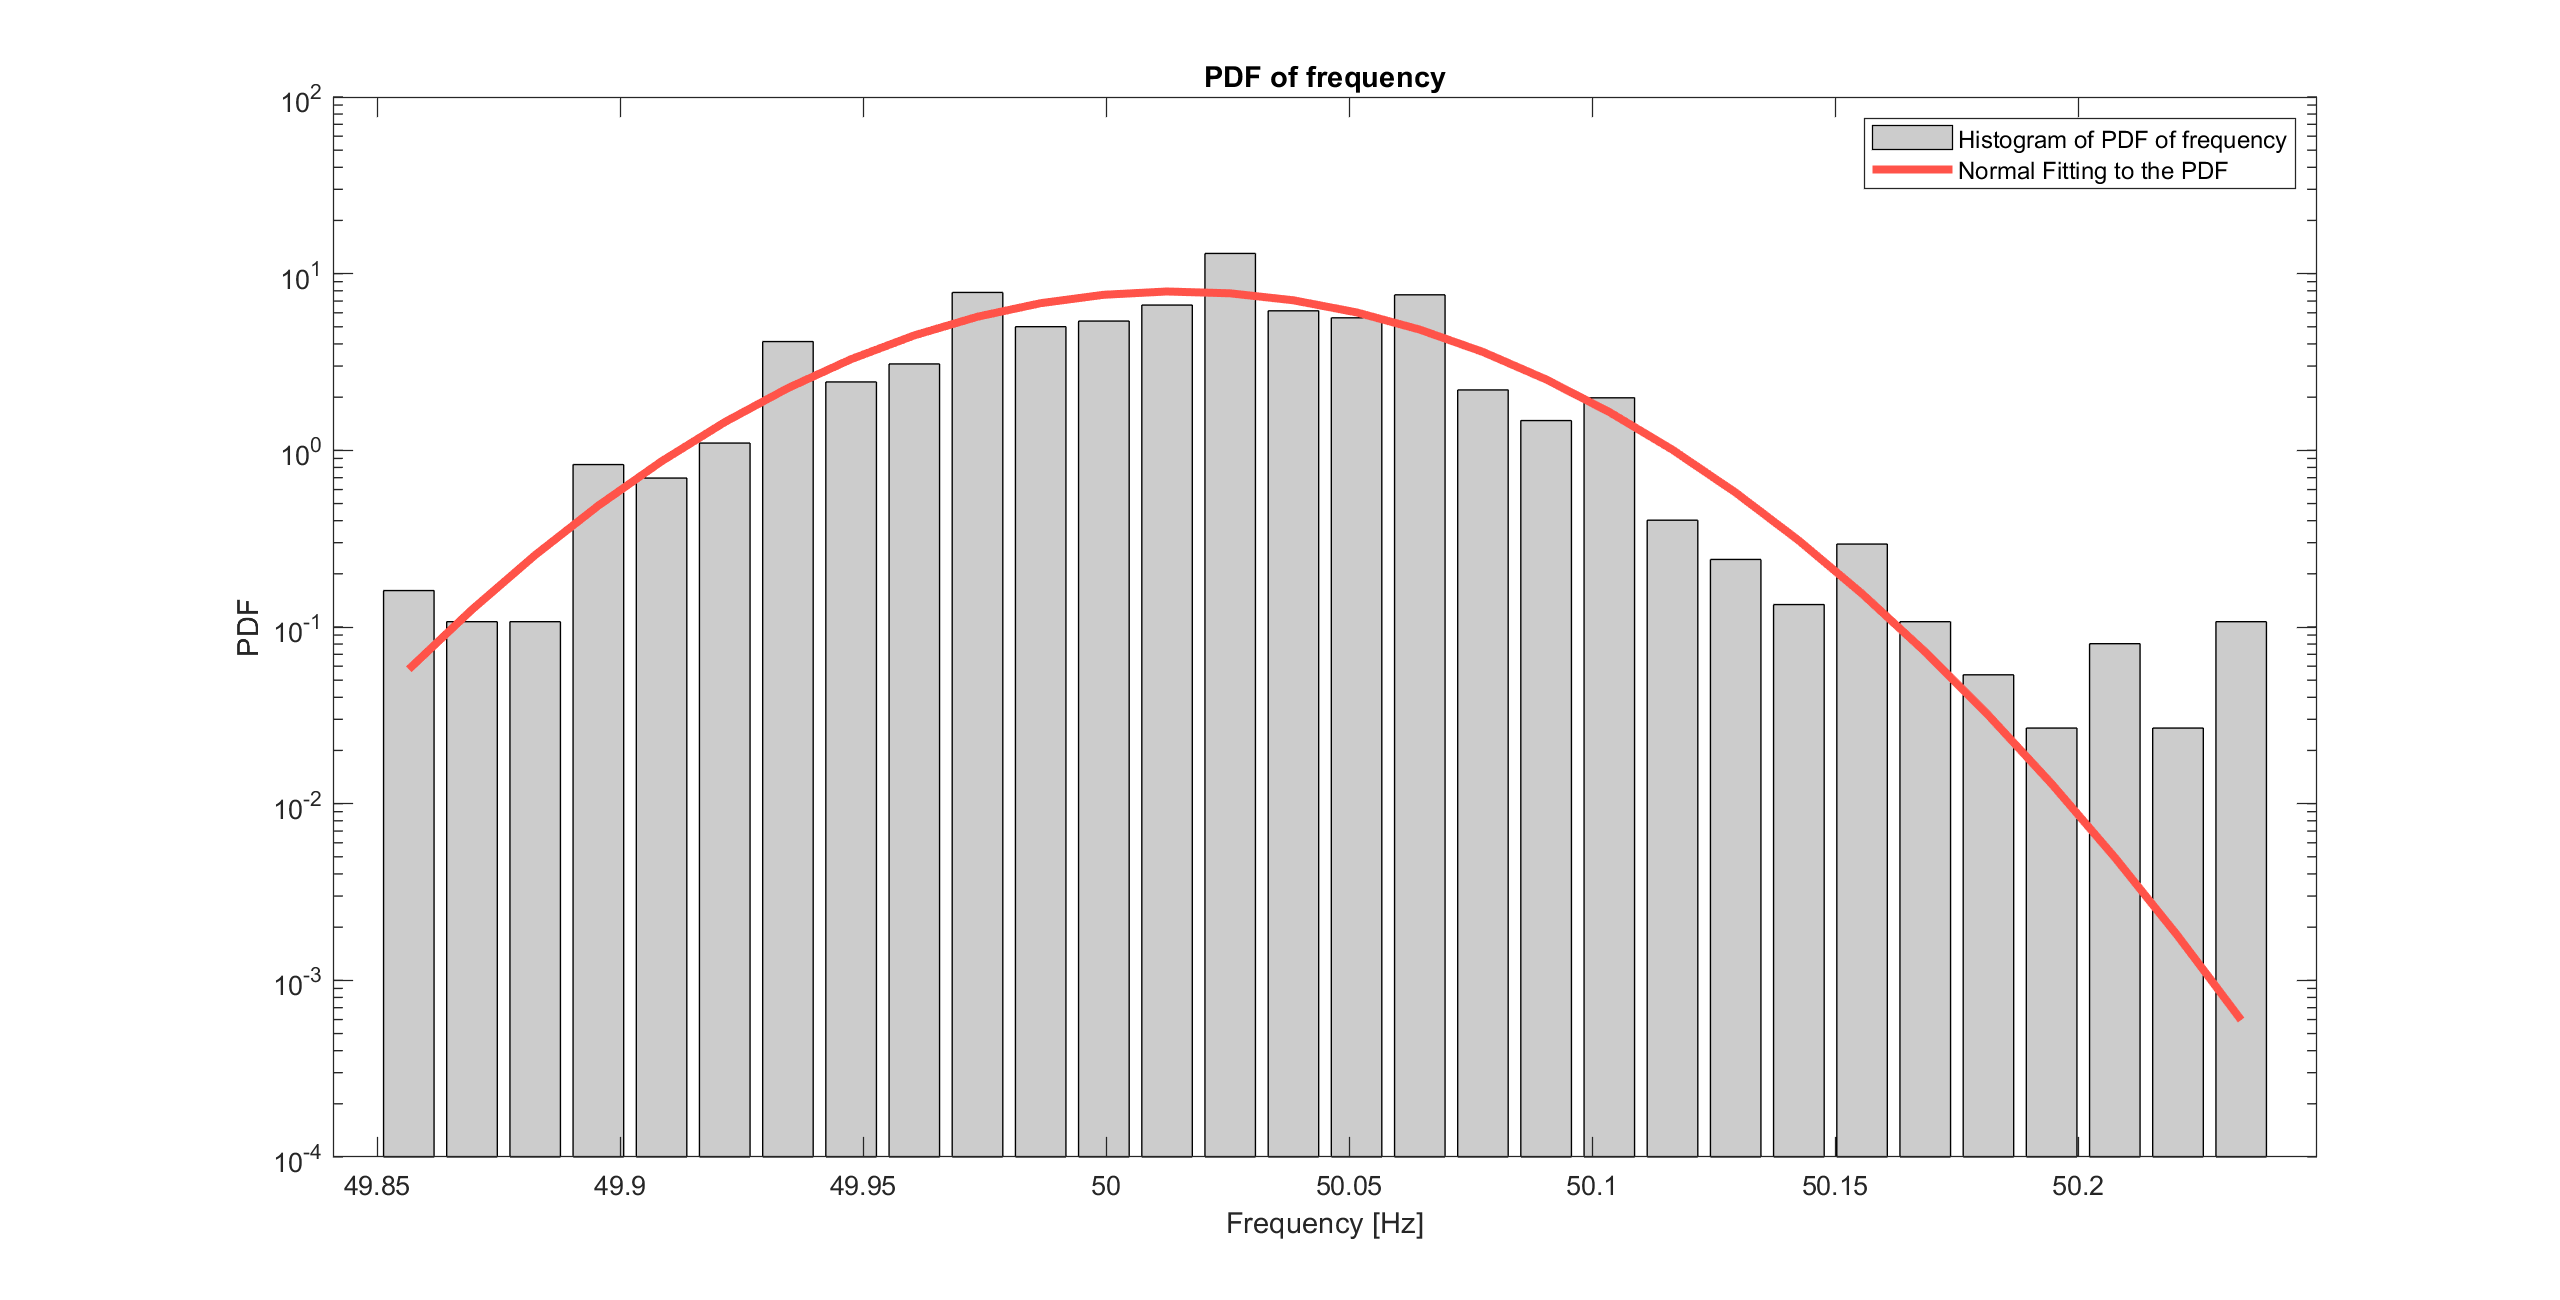
\includegraphics[width=.45\textwidth]{../figures/pdf/nrldc/pdf_frequency_nrldc_04}
	
	\medskip
	
	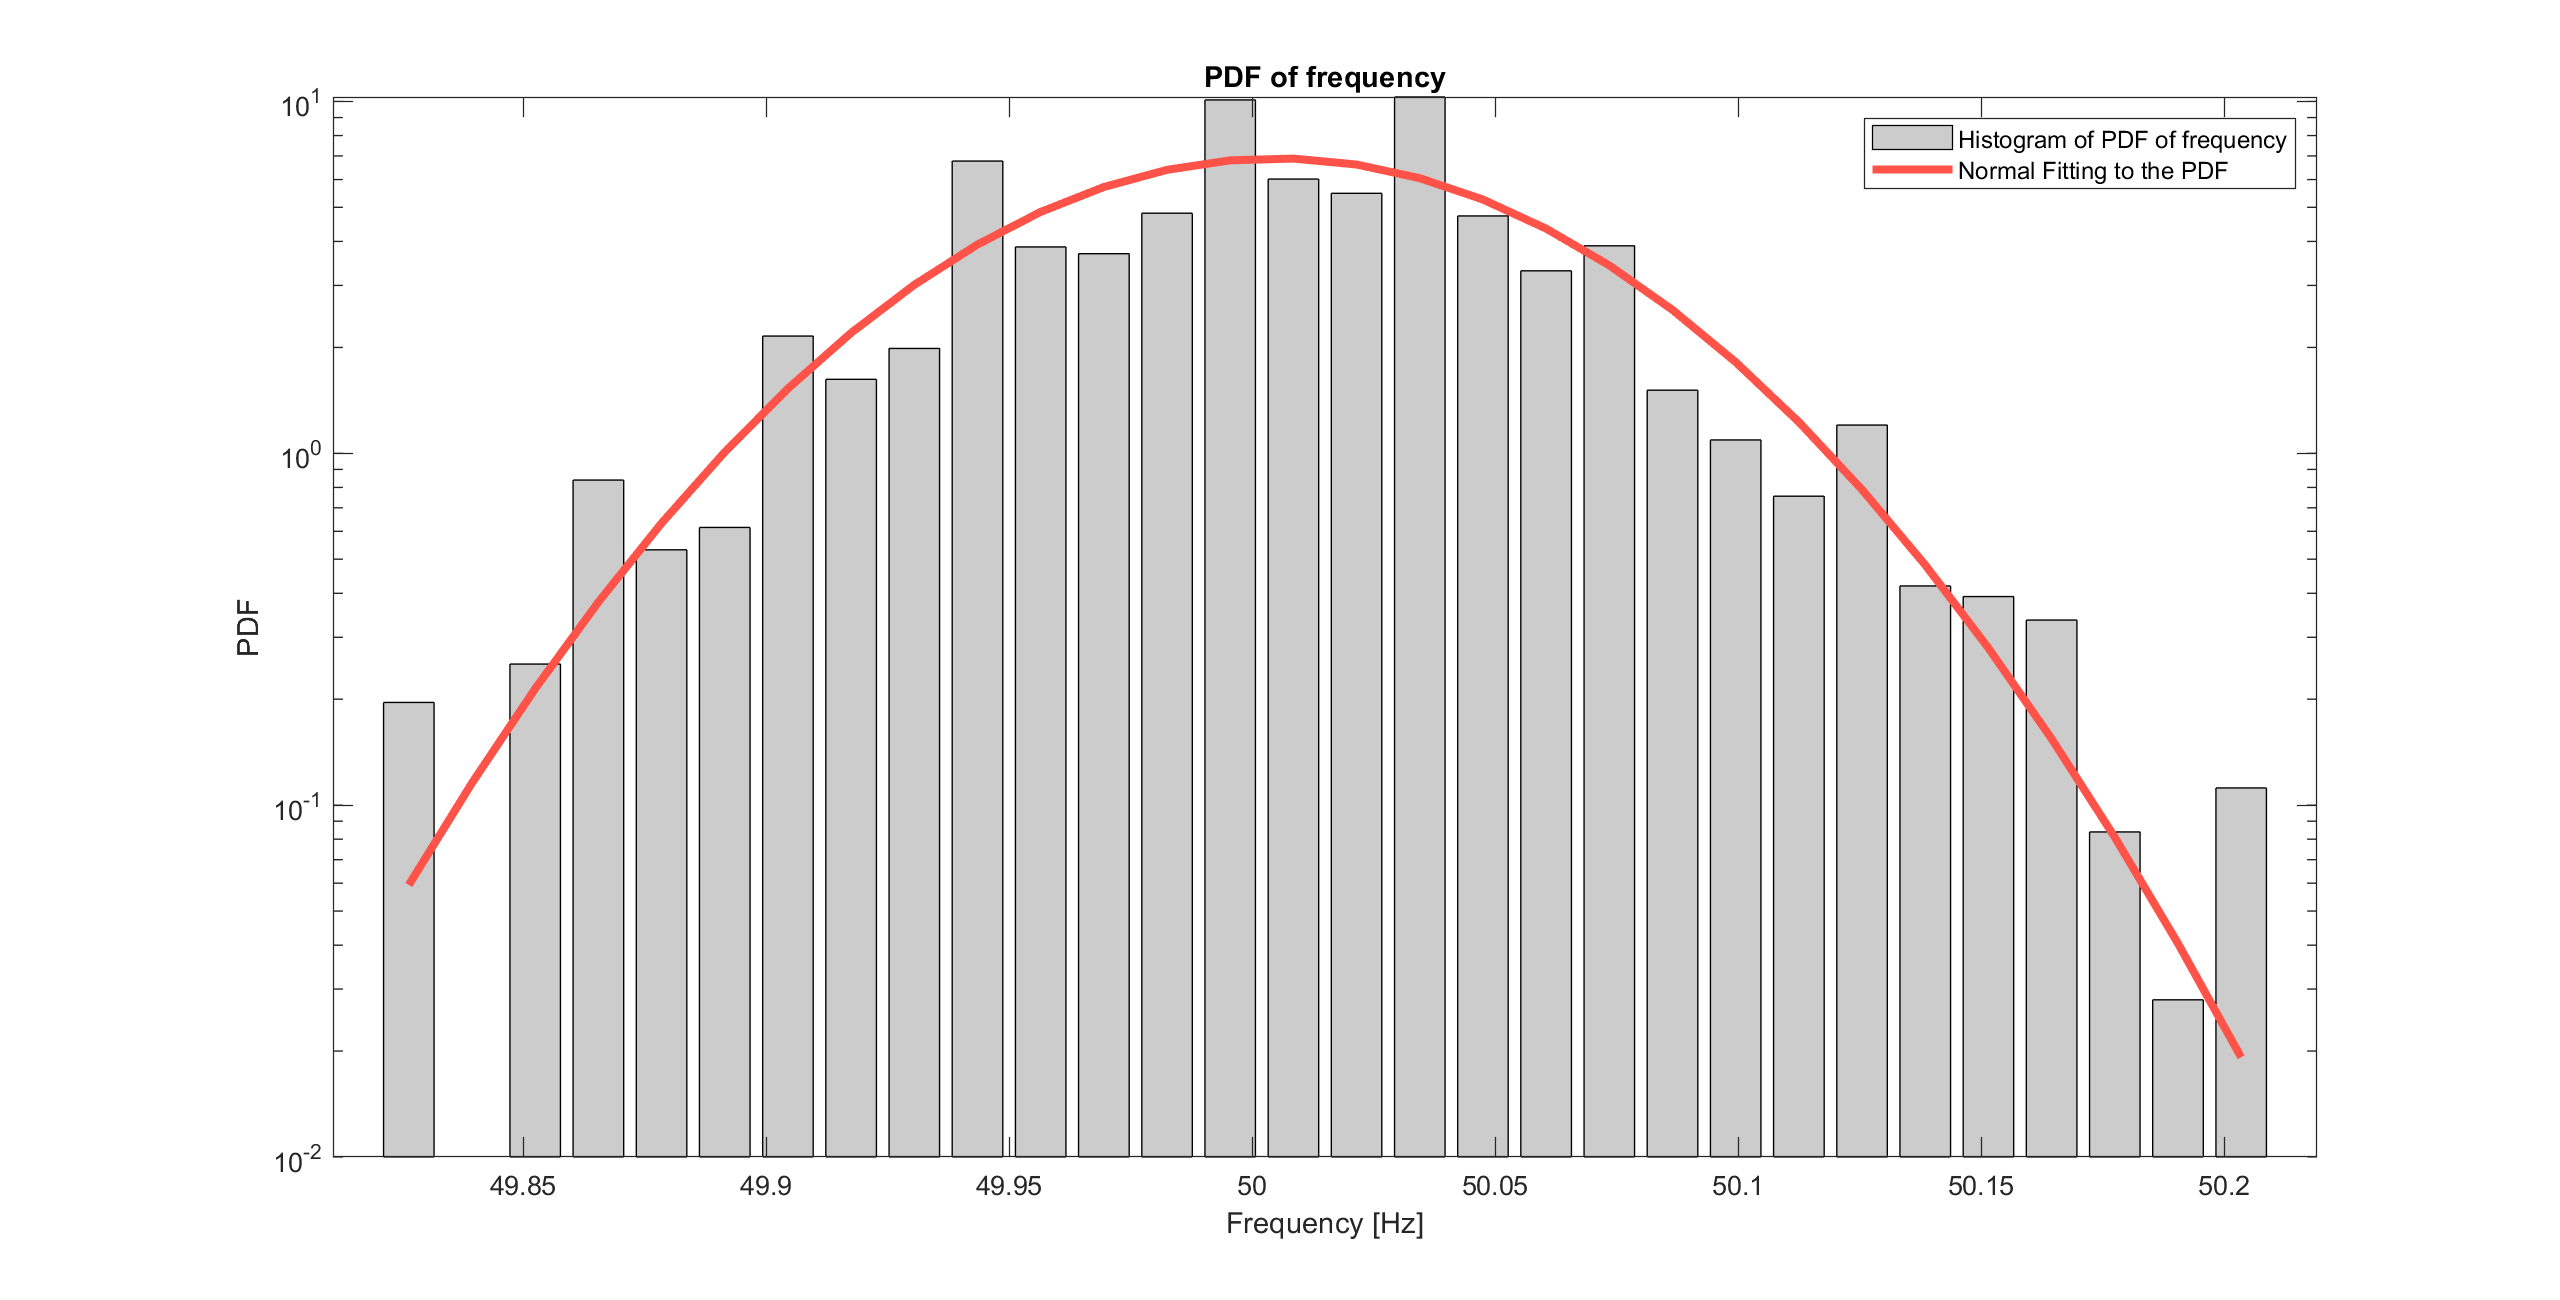
\includegraphics[width=.45\textwidth]{../figures/pdf/nrldc/pdf_frequency_nrldc_05}\quad
	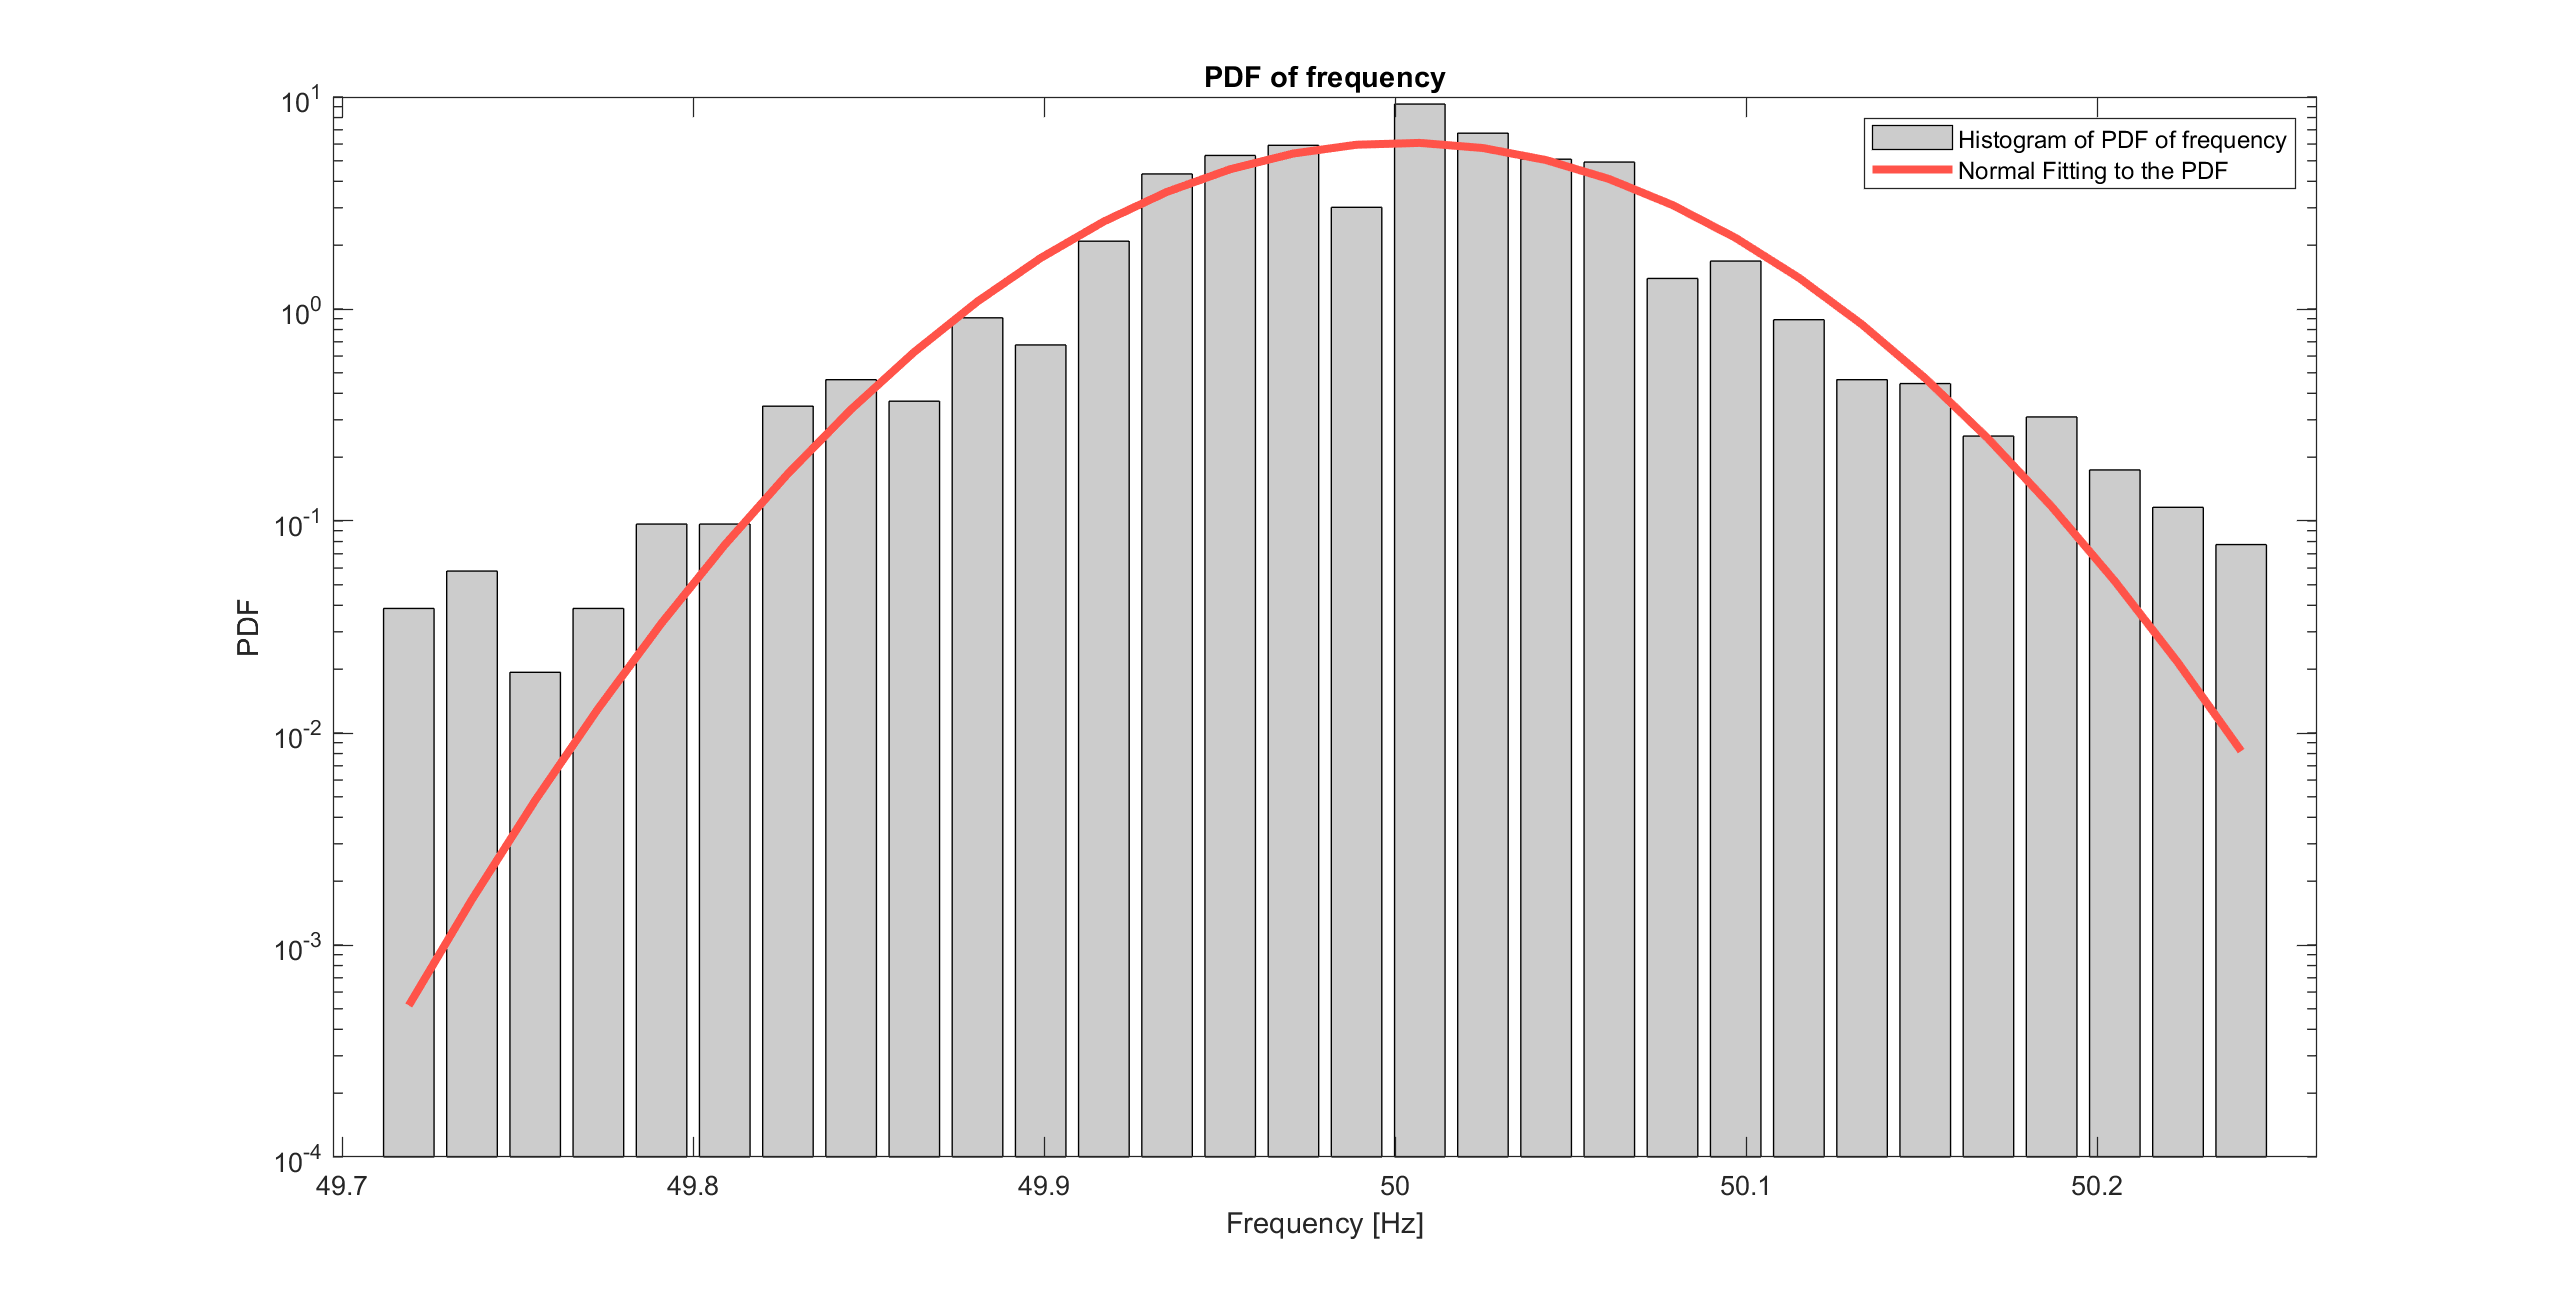
\includegraphics[width=.45\textwidth]{../figures/pdf/nrldc/pdf_frequency_nrldc_06}
	
	\caption{Frequency Probability Density Function Plots for six non-continuous days of the Indian grid (NRLDC). The frequency PDFs show considerable difference among themselves.}
\end{figure}

Similarly, for smaller total sampling durations, the bulk distribution frequency PDF plots are also susceptible to outliers and therefore not ideal for modelling the grid frequency distributions. For example, the available data for the Western Connection Grids and the Texas Grid, both from USA, was small at 3 days and 7 days respectively.

\begin{figure}[!ht]
	\centering
	\begin{subfigure}{\textwidth}
		\centering
		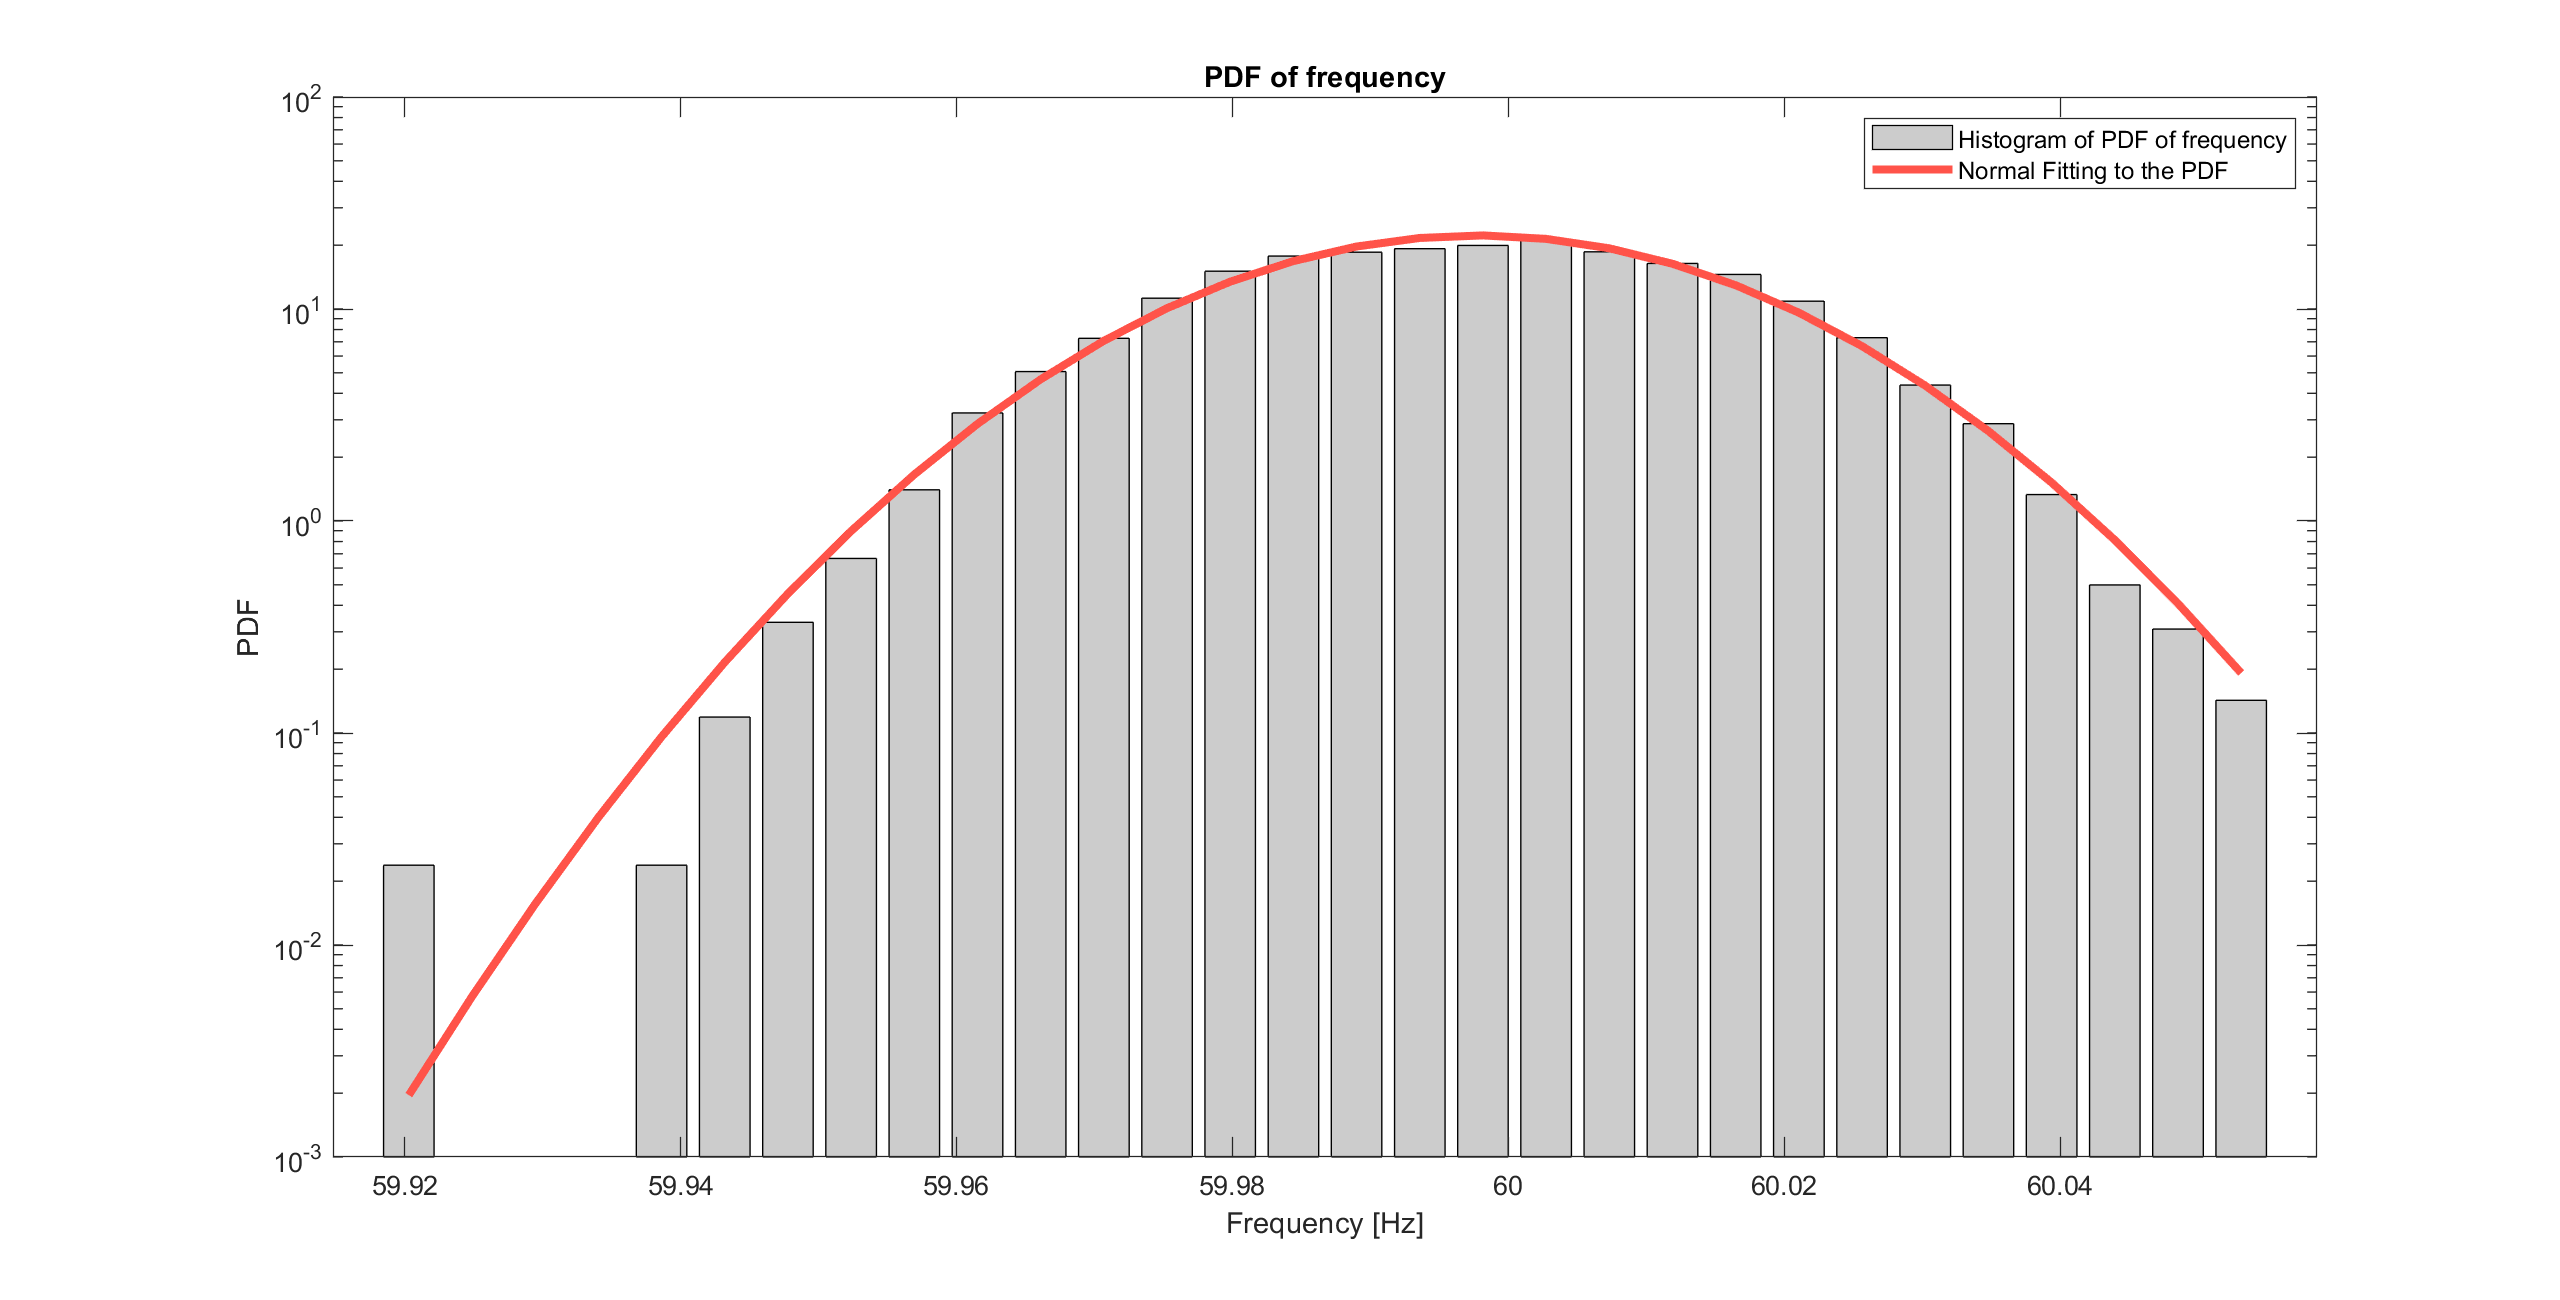
\includegraphics[scale=0.25]{../figures/pdf/pdf_frequency_us_wi_2019_05}
		\caption{Frequency Probability Density Function plot for the Western Interconnection grid in USA for 7 days of May 2019.}
	\end{subfigure}
	
	\begin{subfigure}{\textwidth}
		\centering
		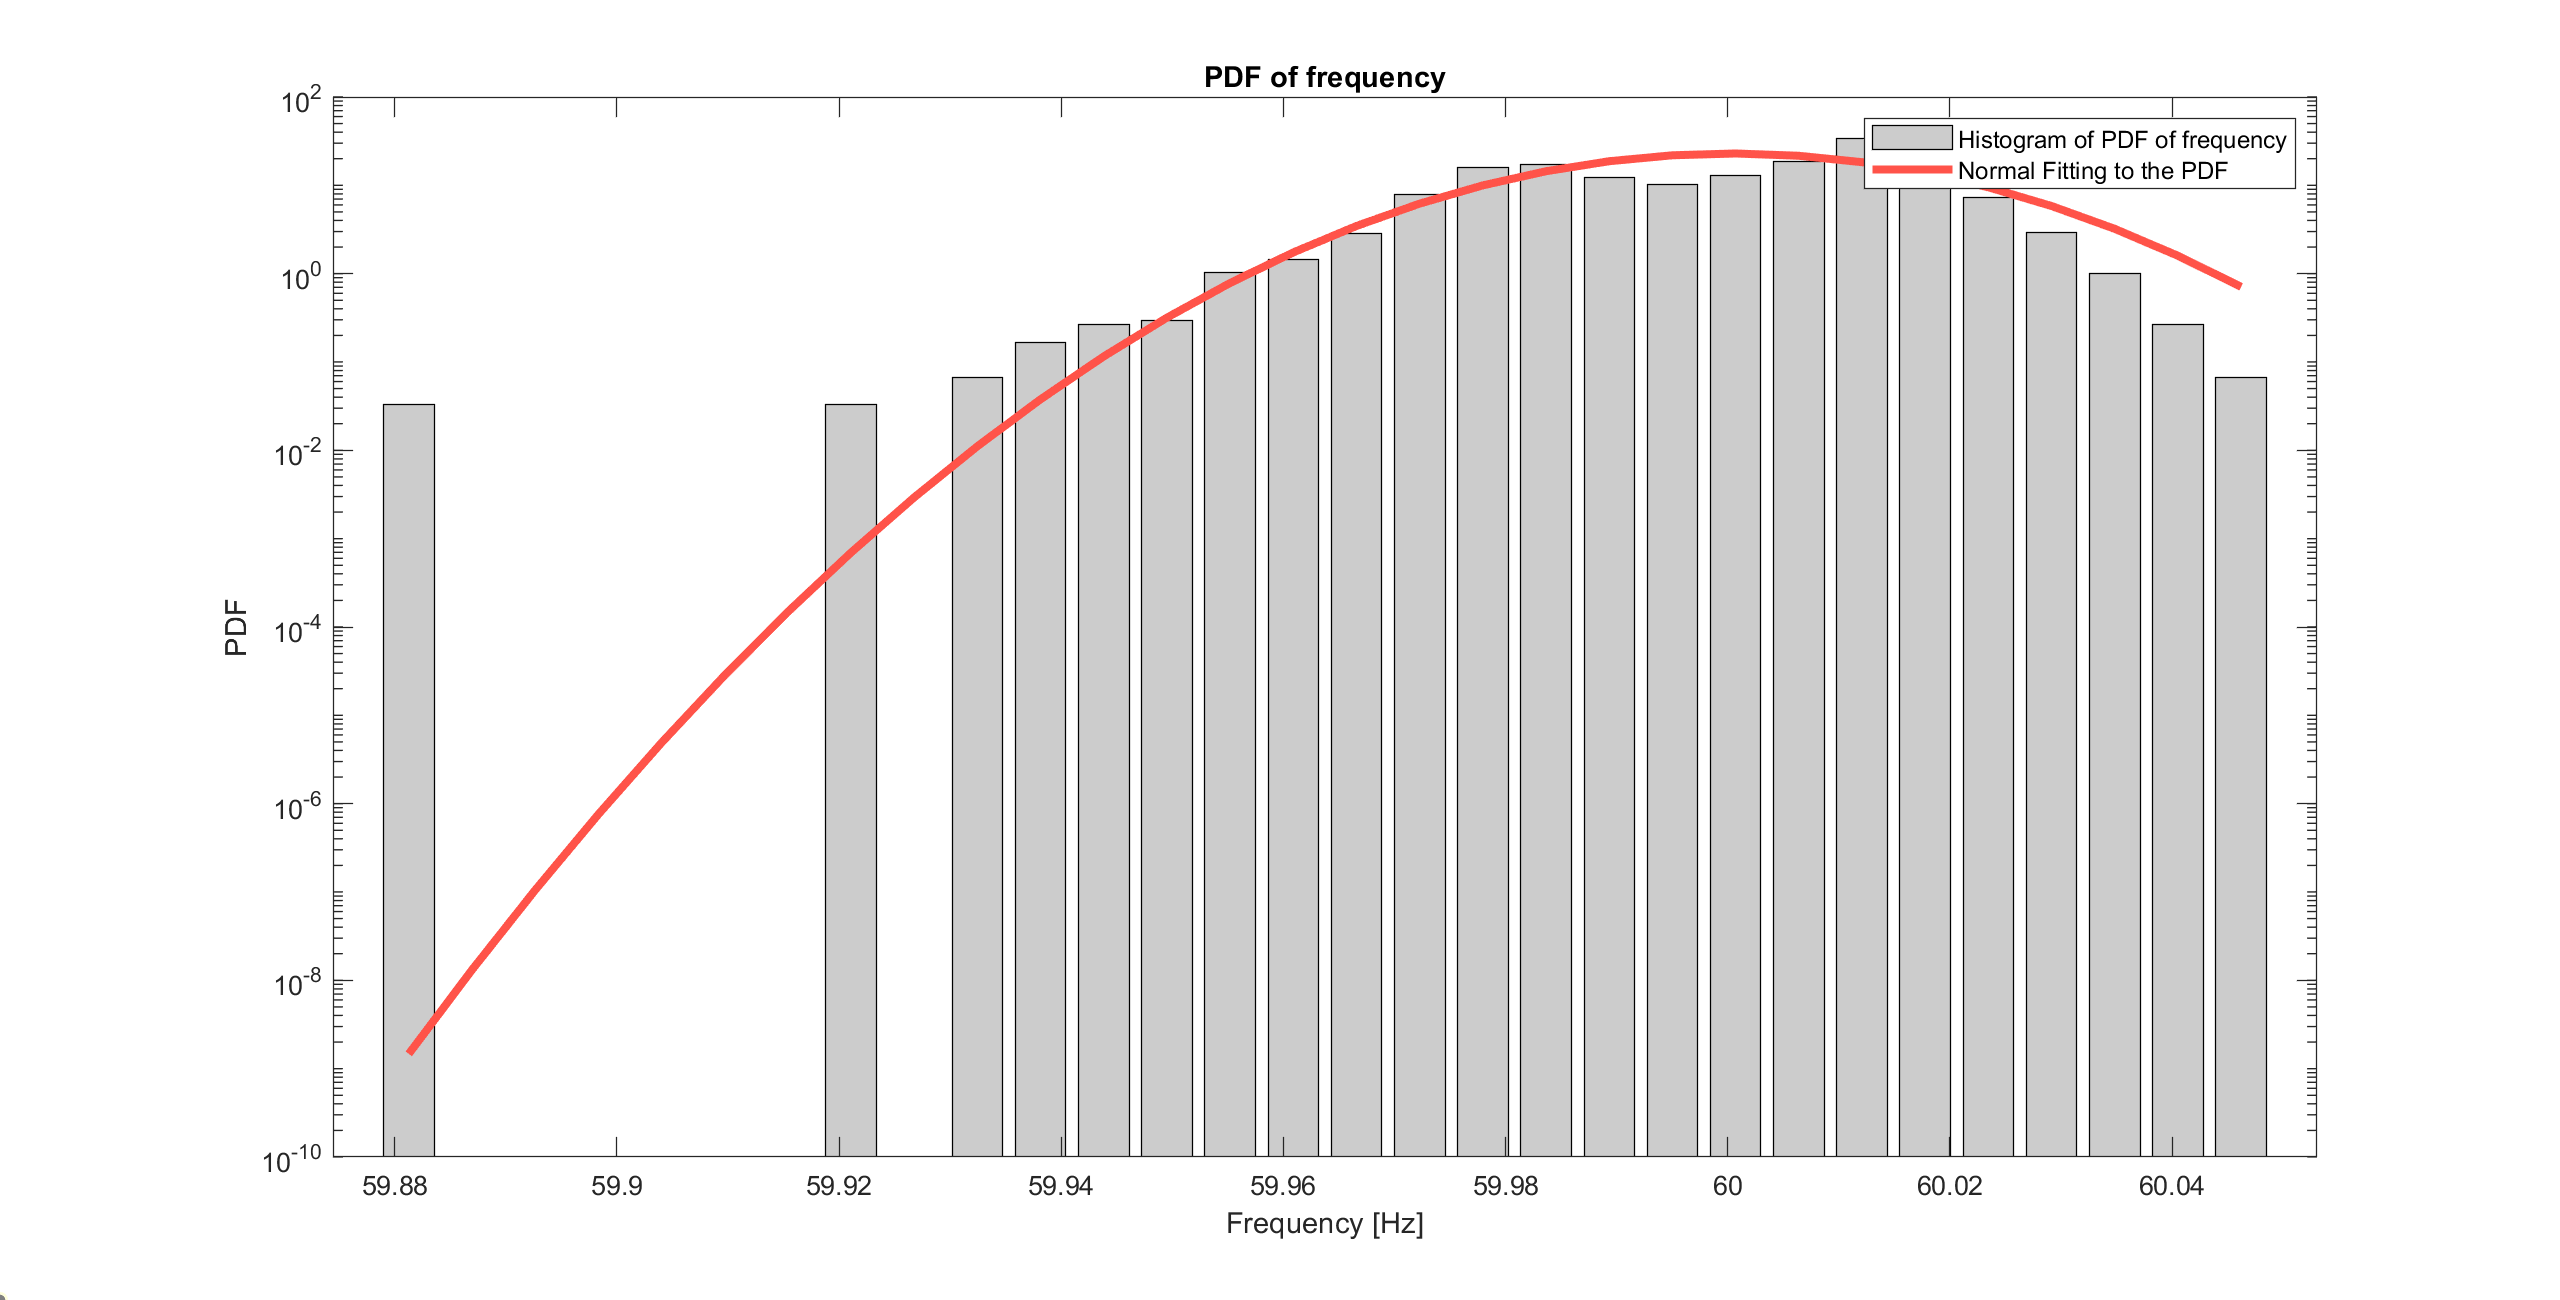
\includegraphics[scale=0.25]{../figures/pdf/pdf_frequency_us_tx_2019_05}
		\caption{Frequency Probability Density Function plot for the Texas Grid for 3 days of May 2019.}
	\end{subfigure}
	\caption{The Texas and Western Interconnection grid frequencies both show outliers in the distribution PDFs, despite not having any faults or major incidences during the sampling period. If the total sampled durations are too low, the frequency distribution PDFs are too susceptible to any major fluctuations, and therefore not reliable models to assume the actual grid frequency distribution PDFs on.}
\end{figure}

Thus a minimum of one month could be considered a sufficient duration to model the bulk characteristics of a grid.

\section[Online/Real-time Analysis]{Online Analysis}
\label{sec:online}

On similar lines as \cite{ghanvati01, sanchez01}, we're interested in testing if symptoms of Critical Slowing Down can be detected by a real-time/online analysis of the state variables of a power grid. In other words, we're interested in checking if computing the autocorrelation and variance of real-time PMU data processed over a running window can provide us with Early Warning Signs of an impending instability.

Bifurcation Theory states that a small change in system parameters, such the governor reference power for a generator ($P_{Gen}$) at certain points, can lead to major upsets in the stability of the power grid. We ran a simulation in which a system was purposefully stressed (via a near constant linear load increment) as time progressed but many restrictions/safety mechanisms were lifted with the aim of singling-out the cause of bifurcation to a change in $P_{Gen}$(s), in order to best demonstrate that the proposed statistical mechanisms (computing autocorrelations and variances) function well as Early Warning Signs even for slow and steady variations of loads, and not just for sudden changes in state variables caused due to reactionary corrective protection mechanisms or the machines not being given `free-range' for chasing load increments due to specified safety limits on maximum allowed generated powers. Below is the set of special conditions used for the simulation of the IEEE 9 Bus system:

\begin{enumerate}
	\item The three load points of the system (Buses 5, 6 and 8) were linearly increased in time, at a rate of $\Delta P \%$ per minute plus a small white noise component $\mathcal{N}(0, \sigma_v)$, with every increment happening at $\Delta t$ time intervals. 
	\begin{equation}
		P_{L_i}(t+\Delta t) = P_{L_i}(t)*\left(1+ \frac{\Delta P_{L_i}}{100}\right) + \mathcal{N}(0, \sigma_v)
	\end{equation} 
	Here, we assigned $\Delta P_{L}$ values randomly between $8-12\%$ for every load bus, $\sigma_v = 0.01$ and $\Delta t = 0.1$ seconds.
	\item Simulation ODE solver solves for the new state variables for the system every $0.01$ seconds. This means that the simulation output can be likened to a stream of PMU data whose sampling rate is $100$ Hz.
	\item Protection mechanisms were disabled. No remedial/corrective action was taken for any drop in bus voltages/grid frequency or any increase in line currents/MVAs.
	\item `Dummy' governors were placed on the three generators (at buses 1, 2 and 3) which could respond instantly to load changes by changing the set reference generation powers $P_{Gen}$(s) with zero time lag.
	\item The generator limits for $P_{Gen_{MAX}}$, $Q_{Gen_{MAX}}$, etc. were removed. Thus the generators had complete freedom to `chase' the load increments at the load buses, including factoring in the extra line-losses.
\end{enumerate} 

It should be noted that while autocorrelation was used in both online/real-time and offline/postmortem analyses, the two usages were different in:

\begin{itemize}
	\item their mode of procuring and processing input data (a running window of an incoming stream of data vs previously stored months/years worth of time series),
	\item the degrees of freedom allowed for its two parameter variables (which out of $t$ and $\tau$ is allowed to be constant),
	\item their theoretically expected output data (autocorrelation is should decrease exponentially with respect to time lag $\tau$ but increase with time $t$ if that the system is being progressively stressed with time)
\end{itemize} 
 
 

\section[Conclusions]{Conclusions}
\label{sec:concl}

\lipsum[2]

\section[Future Work]{Future Work}
\label{sec:future}

Despite the successful application of statistical analysis to detect symptoms of Critical Slowing Down in various phenomena \cite{schefferEarlyWarningSignalsForCriticalTransitions}, autocorrelation and variance are not certain indicators for the same, at least by themselves \cite{csdNotDetectedByAutocorrAndVariance01}.


\section{References}
\label{sec:references}

\begin{frame}[allowframebreaks]{References}
		\printbibliography[heading=none]
\end{frame}

\section{Proposed Contents of the Thesis}
The outline of the thesis is as follows:
\begin{enumerate}
\item Introduction and Literature Review
\item Motivation and Objectives
\item Theory
\item Offline/Postmortem Analysis
\item Online/Real-time Analysis
\item Conclusions
\item Future Work
\item References
\end{enumerate}


\end{document}

